\documentclass[10pt]{beamer}%
\usetheme[progressbar = foot]{metropolis} 
\usecolortheme[cautious]{owl} %owl-defined colours will be available as OwlRed, OwlGreen, and so forth.
\setbeamercolor{title separator}{fg=OwlGreen}

% input

\usepackage[utf8]{inputenc}%
\usepackage{lmodern} %Type1-font for non-english texts and characters
\usepackage[USenglish]{babel} %francais, polish, spanish, ...
\usepackage[T1]{fontenc}

\usepackage{ragged2e}%for text justification by default
\justifying

% graphics
%% Figures %%%%%%%%%%%%%%%%%%%%%%%%%%%%%%%%%%%%%%%%%%%%%%%%%%
\usepackage{graphicx}
\usepackage{xcolor}%for color mixing
\definecolor{mypurple}{rgb}{0.231, 0.204, 0.471}
\definecolor{mypurple1}{rgb}{0.573, 0.467, 0.675}
\definecolor{mypurple2}{rgb}{0.122, 0.016, 0.224}

\definecolor{mygreen}{rgb}{0.153, 0.443, 0.365}
\definecolor{myorange}{rgb}{0.882, 0.612, 0.224}

\definecolor{bostonuniversityred}{rgb}{0.8, 0.0, 0.0}
\definecolor{blendedblue}{rgb}{0.137,0.466,0.741}

\definecolor{darkred}{rgb}{0.545,0,0}

 
\usepackage{tikz} % for arrows and figures
\usetikzlibrary{positioning,decorations.pathreplacing,shapes,trees,calc}

\makeatletter
\newcommand{\gettikzxy}[3]{%
  \tikz@scan@one@point\pgfutil@firstofone#1\relax
  \edef#2{\the\pgf@x}%
  \edef#3{\the\pgf@y}%
}

\usepackage{amsmath}%
\usepackage{amsfonts}%
\usepackage{amssymb}%
\usepackage{graphicx}


\usepackage{booktabs}


\usepackage{hyperref}
\setlength{\arraycolsep}{3pt}

%%%%%%%%%%%%%%%%%%%%%%%%%%%%%%%%%%%%%%%%%%%%%%
%%%%%%%%%%%%%%%%% Doc info %%%%%%%%%%%%%%%%%%%
\title[\textbf{Adaptation against apparent selection}]{\textbf{Individual-level causes and population-level consequences of variation in fitness in an Alpine rodent}}
%\titlegraphic{\fcolorbox{blendedblue}{blendedblue}{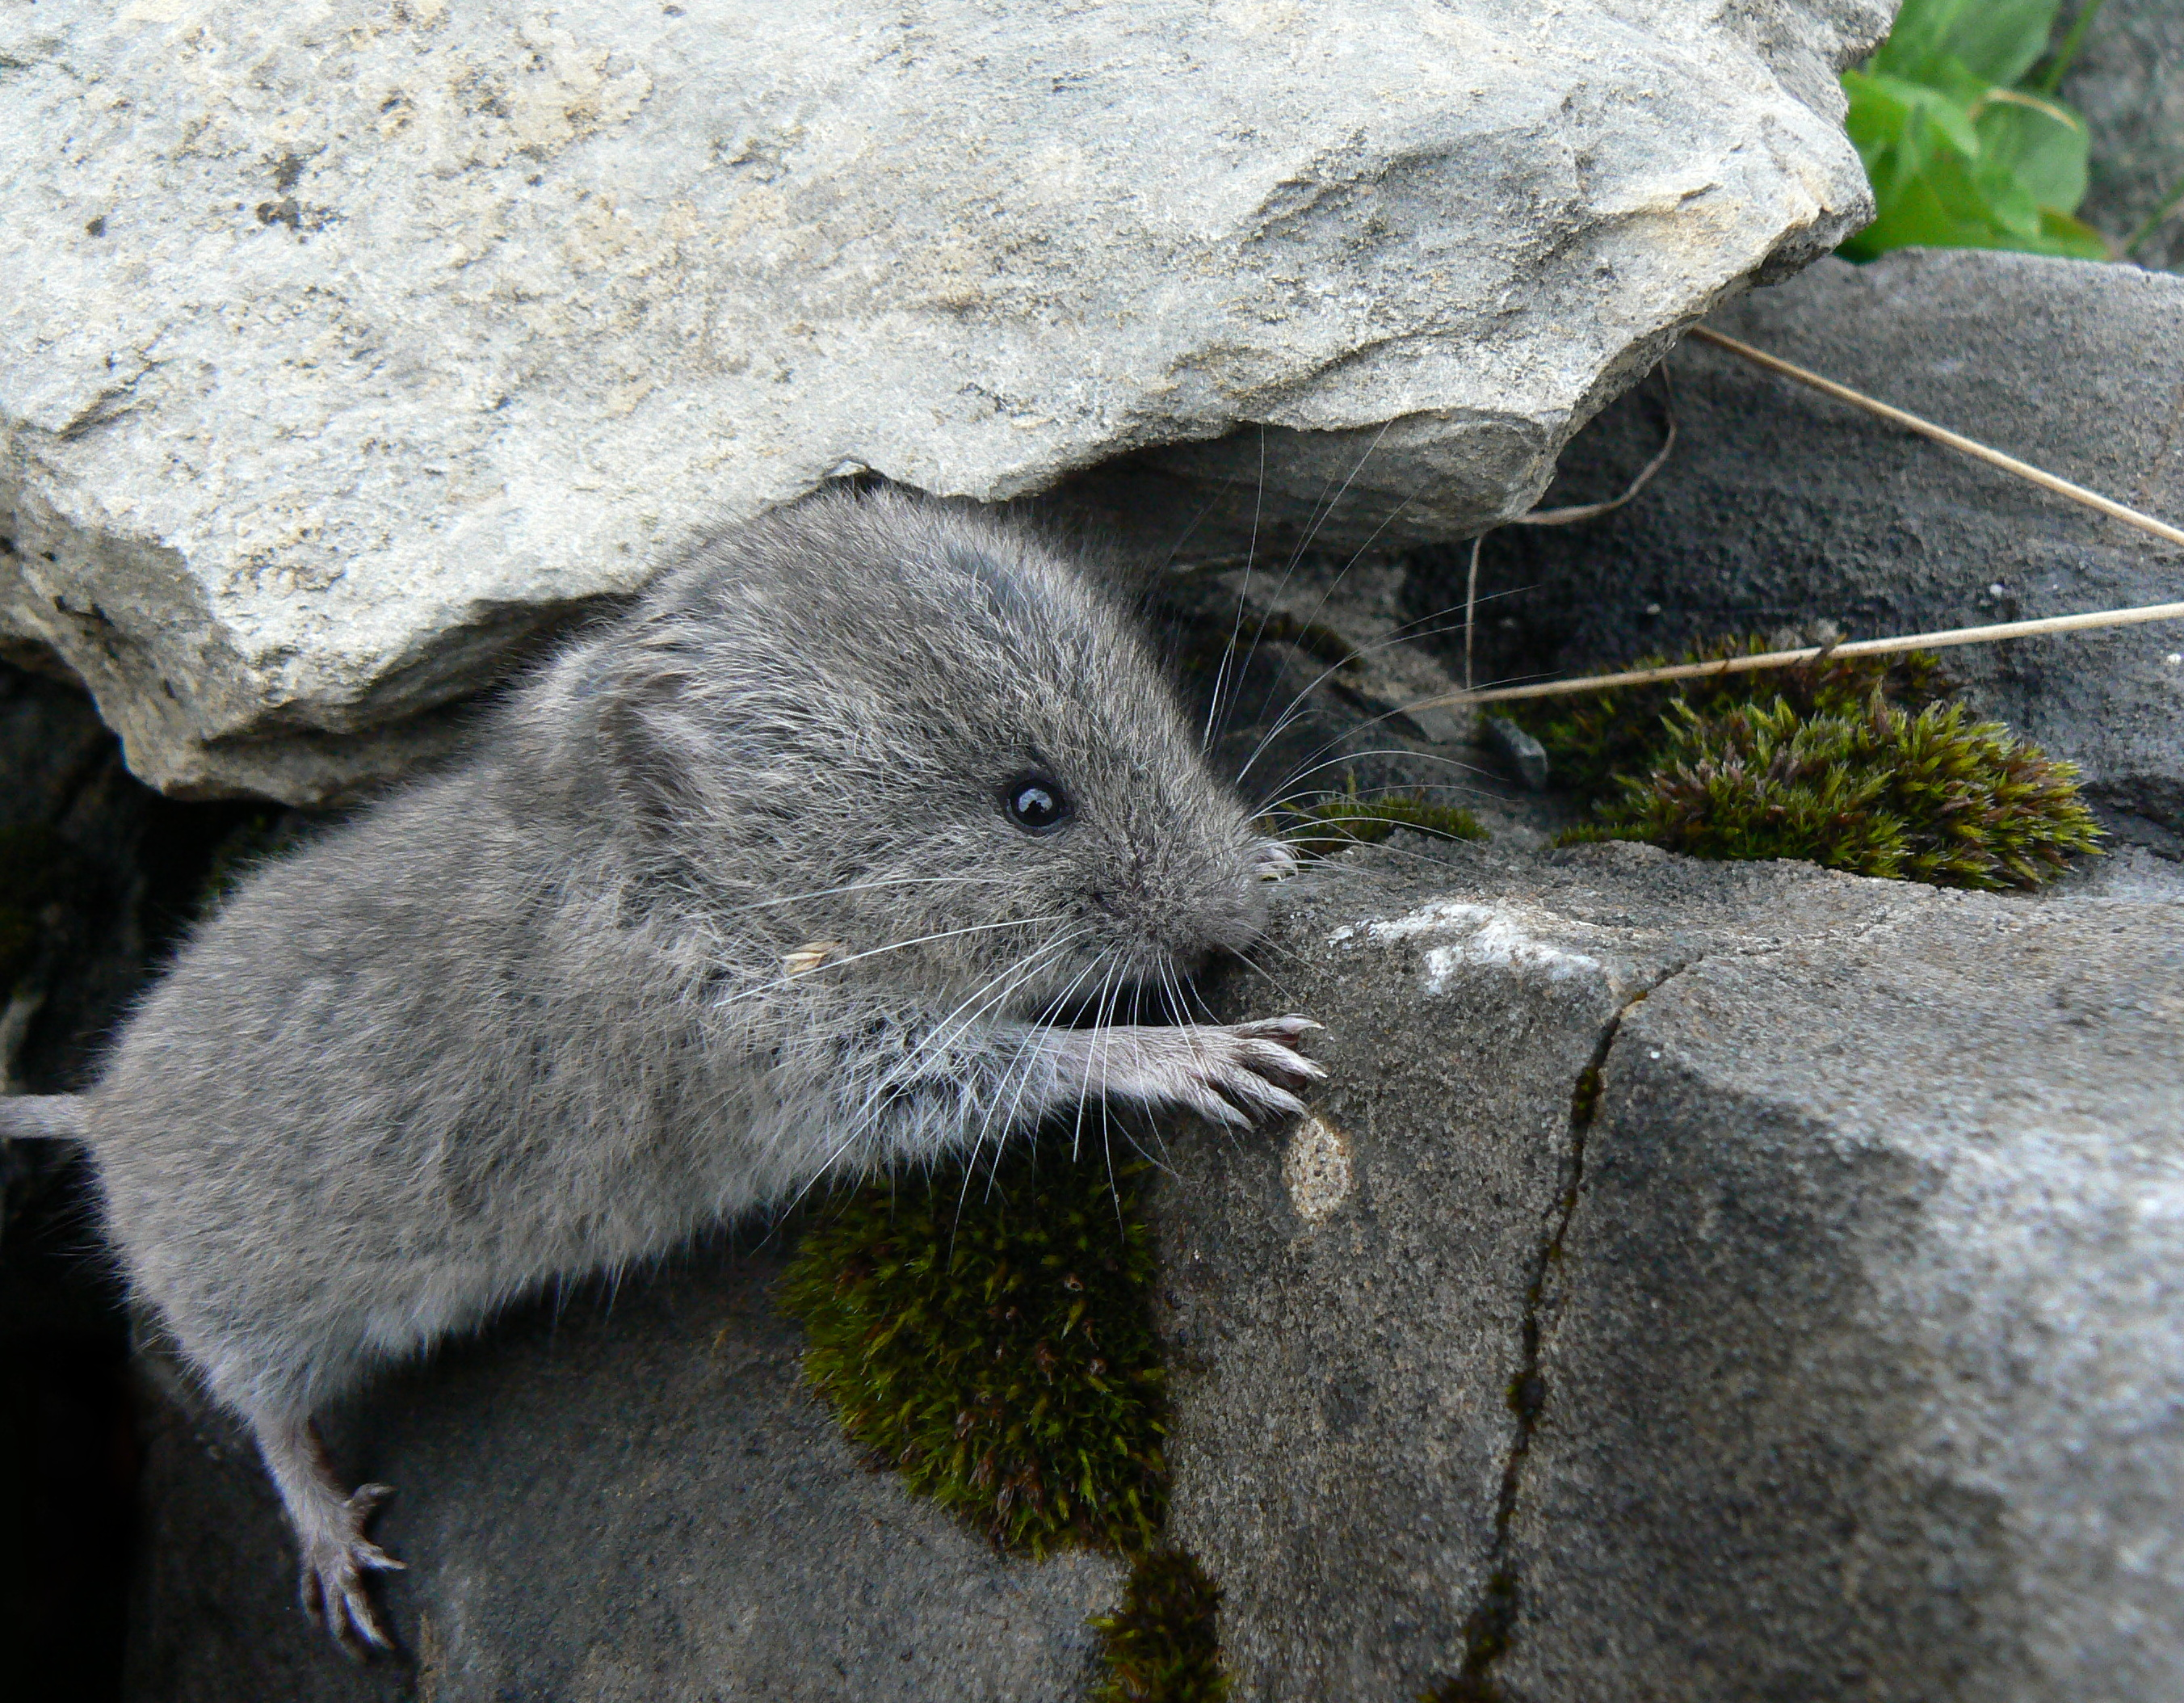
\includegraphics[width=0.45\textwidth]{Figures/cutevole}}}
%\subtitle{UOBU}
\author[\textbf{\fontfamily{pcr}\selectfont timothee.bonnet@ieu.uzh.ch}]{\textbf{Timoth\'{e}e Bonnet}}
%\date{\fcolorbox{blendedblue}{blendedblue}{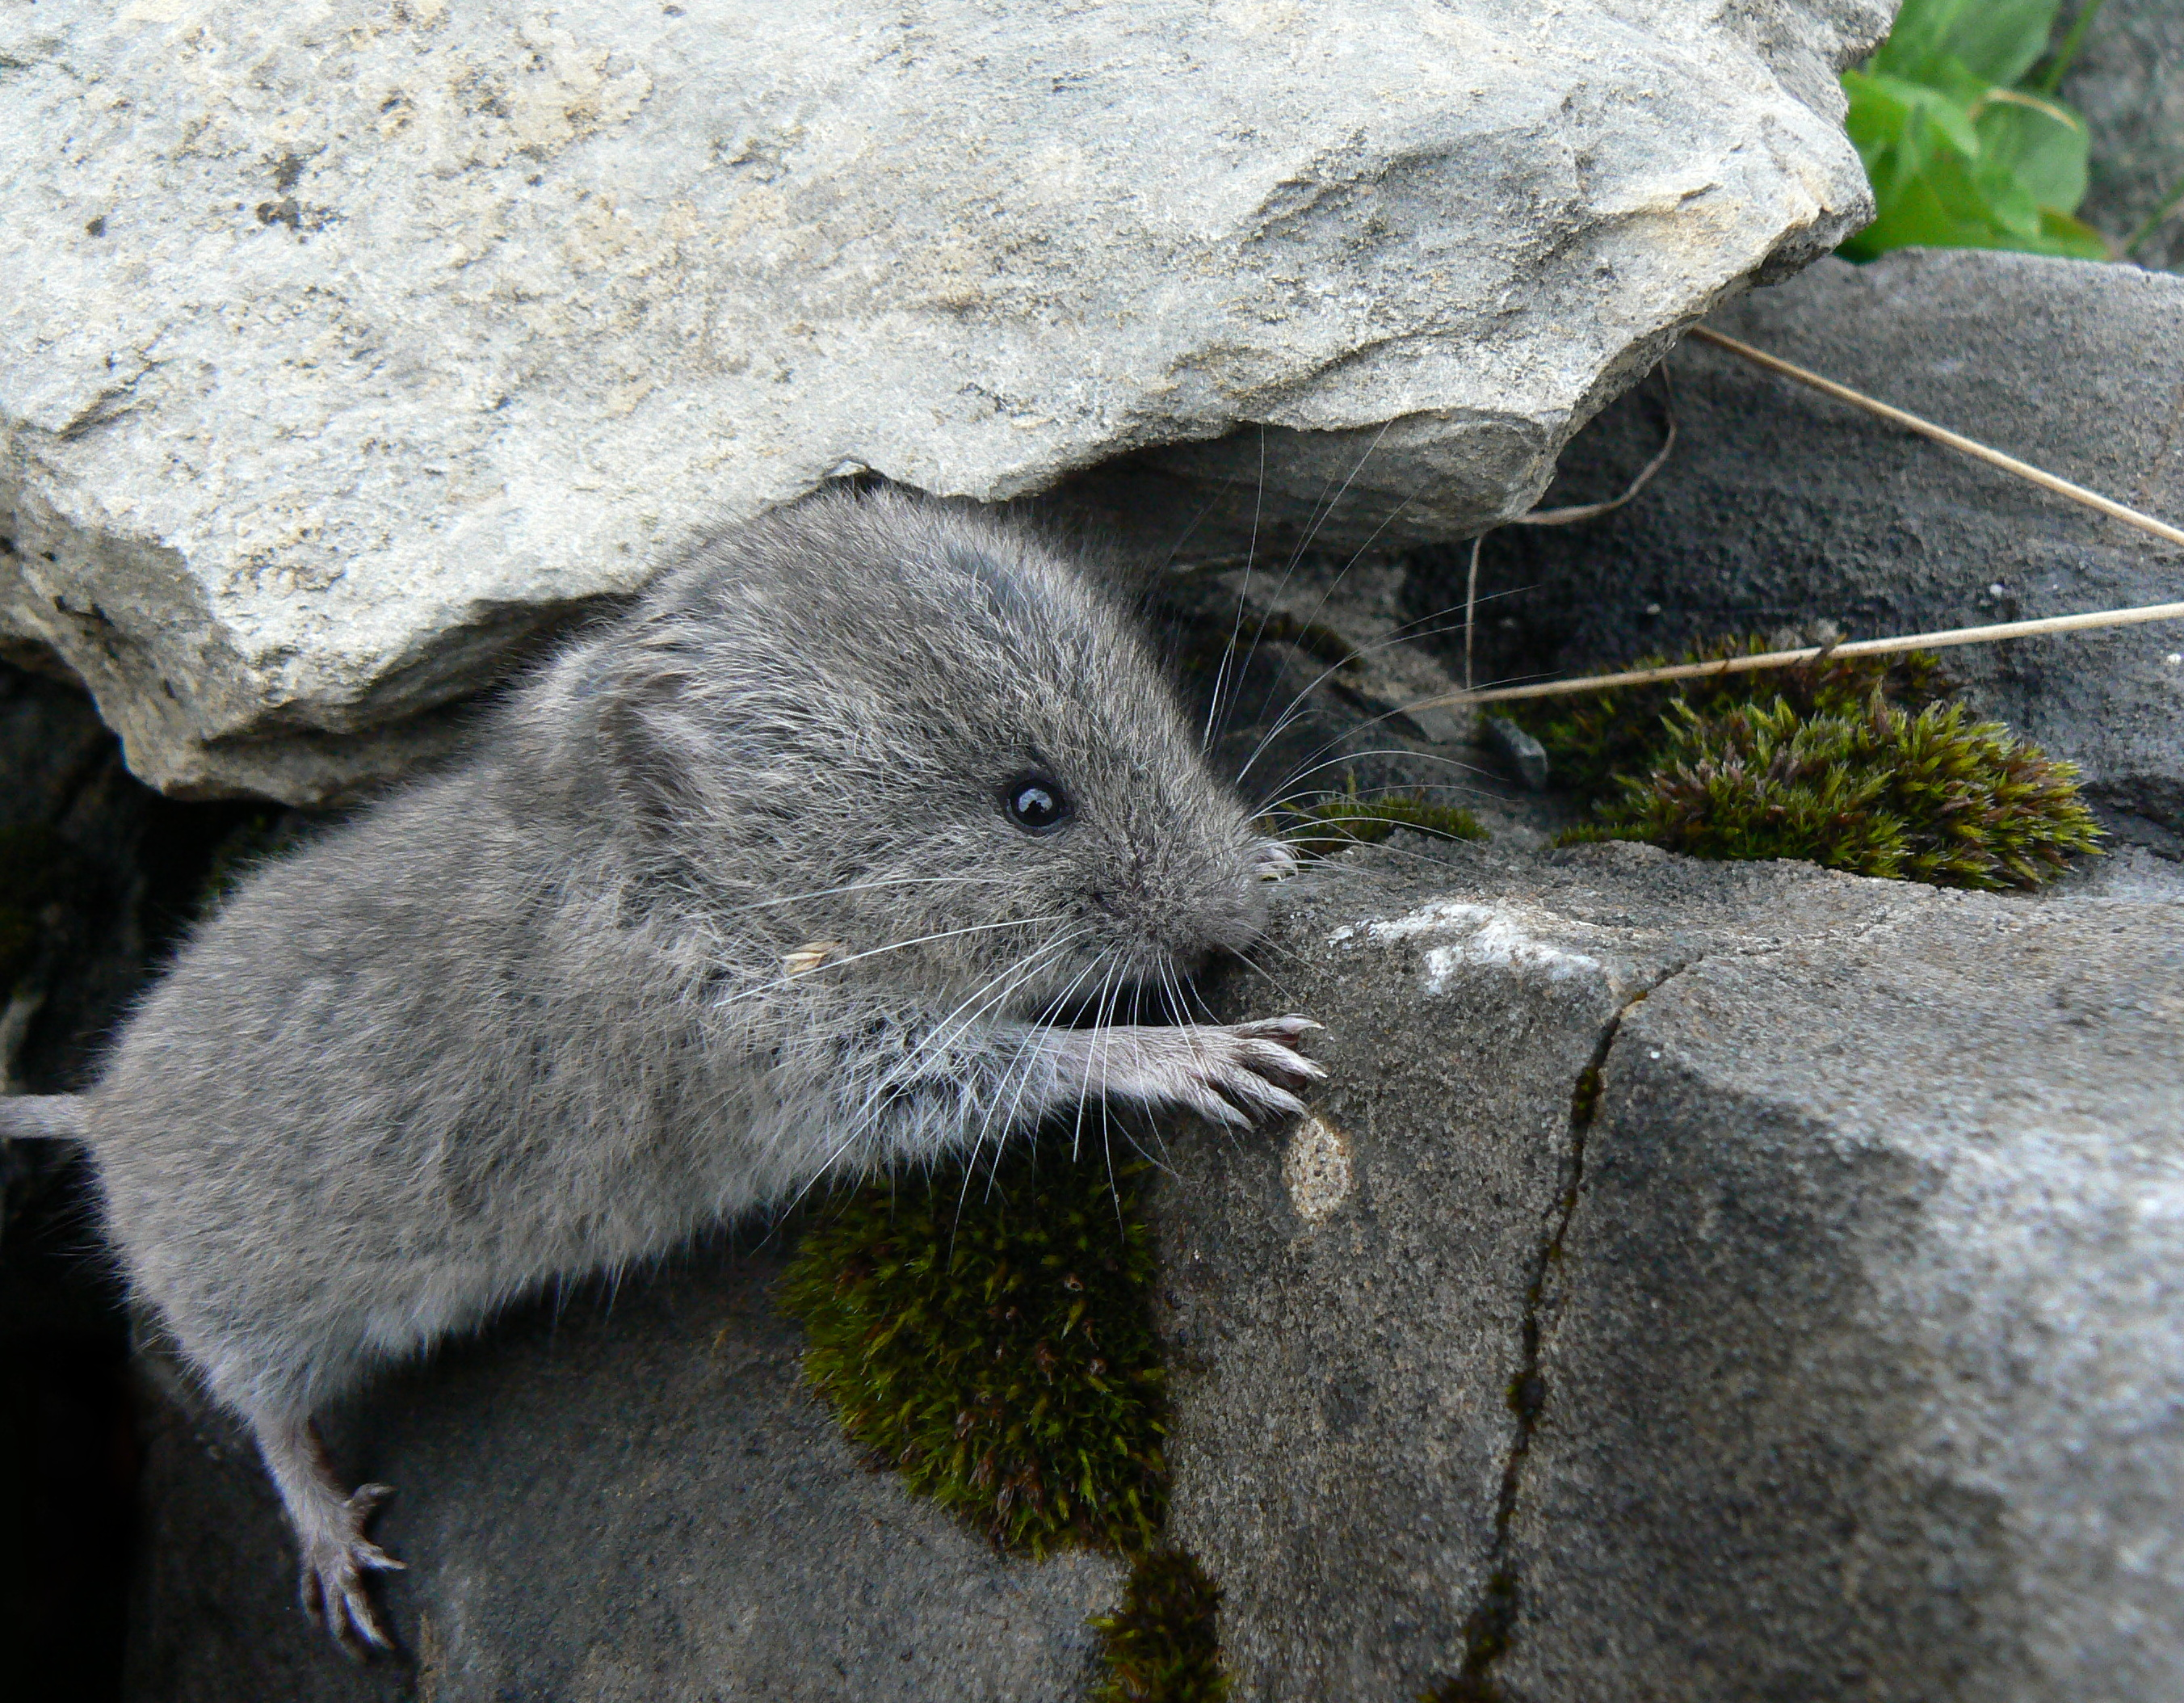
\includegraphics[width=0.35\textwidth]{Figures/cutevole}}}
\date{\vspace{1cm}}
\institute[IEU, University of Zurich]{\small Department of evolutionary biology and environmental studies (IEU) \\ \vspace{-0.1cm} \\ 
\includegraphics[width=0.3\textwidth]{Figures/uzh_logo_e_neg}}



%%%%%%%%%%%%%%%%%%%%%%%%%%%%%%%%%%%%%%%%%%%%%%
\begin{document}

\begin{frame}[plain]
\maketitle
\end{frame}
%%%%%%%%%%%

%\section{Acknowledgements}

\begin{frame}[plain]

\begin{columns}
	\begin{column}[c]{0.35\textwidth}
		\begin{itemize}
		\setlength\itemsep{0.05cm}
		\small
			\item<2-> Erik Postma
		%committee
			\item<3-> Lukas Keller
			\item<3-> Barbara Tschirren
			\item<3-> Arpat Ozgul
			\item<3-> Marc Kéry 
			\item<3-> Jarrod Hadfield
		%colleagues
			\item<4-> Glauco Camenisch
			\item<5-> Ursina Tobler
			\item<6-> Dominique Waldvogel
			\item<6-> Martina Schenkel
			\item<6-> Vicente Garc{\'{i}}a-Navas
			\item<7-> Andres Hagmayer
			\item<8-> Koen van Benthem
			\item<8-> Marjolein Bruijning
			\item<8-> Eelke Jongejans	
			\item<9-> Pirmin Nietlisbach
			\item<9-> Philipp Becker
			\item<9-> Judith Bachmann
					
%former colleagues?

%friends and family
		\end{itemize}
	\end{column}
	\begin{column}[c]{0.7\textwidth}
		%Residual
		\begin{figure}[c]
			\begin{tikzpicture}
				\uncover<2->{\node (erik) at (0,0) {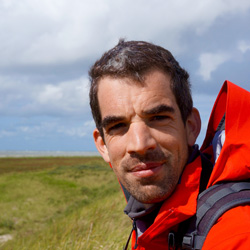
\includegraphics[width = 0.2 \textwidth]{Figures/Erik}};}
				\uncover<3->{\node (lukas) at ($(erik)+(1.2,0)$) {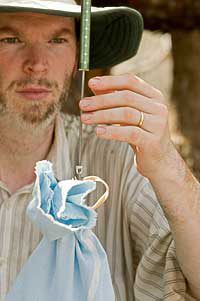
\includegraphics[width = 0.15 \textwidth]{Figures/Lukas}};
				\node (barbara) at ($(lukas)+(1,0)$) {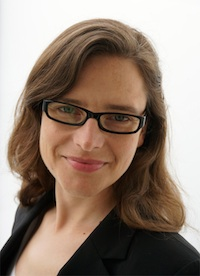
\includegraphics[width = 0.15 \textwidth]{Figures/Barbara}};
				\node (arpat) at ($(barbara)+(1.3,0)$) {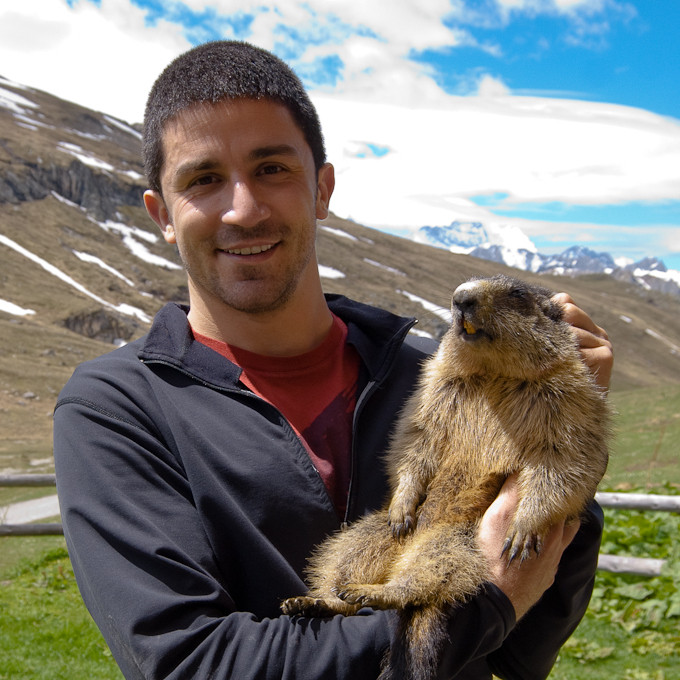
\includegraphics[width = 0.2 \textwidth]{Figures/Arpat}};
				\node (marc) at ($(arpat)+(1.2,0)$) {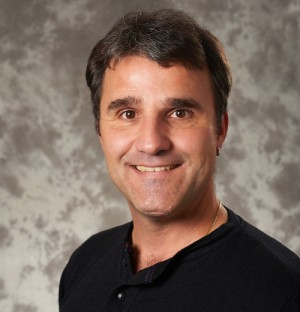
\includegraphics[width = 0.2 \textwidth]{Figures/Marc}};
				\node (jarrod) at ($(marc)+(1.3,0)$) {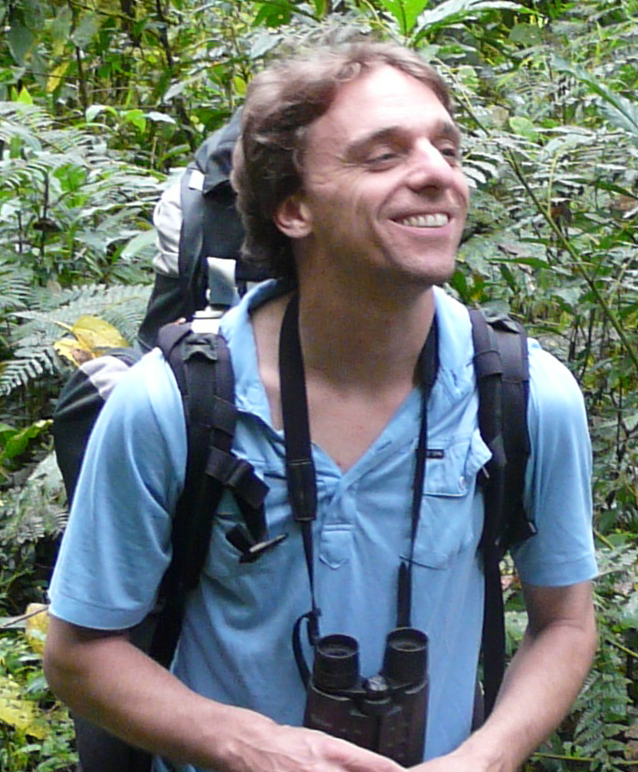
\includegraphics[width = 0.2\textwidth]{Figures/Jarrod}};}
				\uncover<4->{\node (glauco) at ($(erik)+(0,-1.4)$) {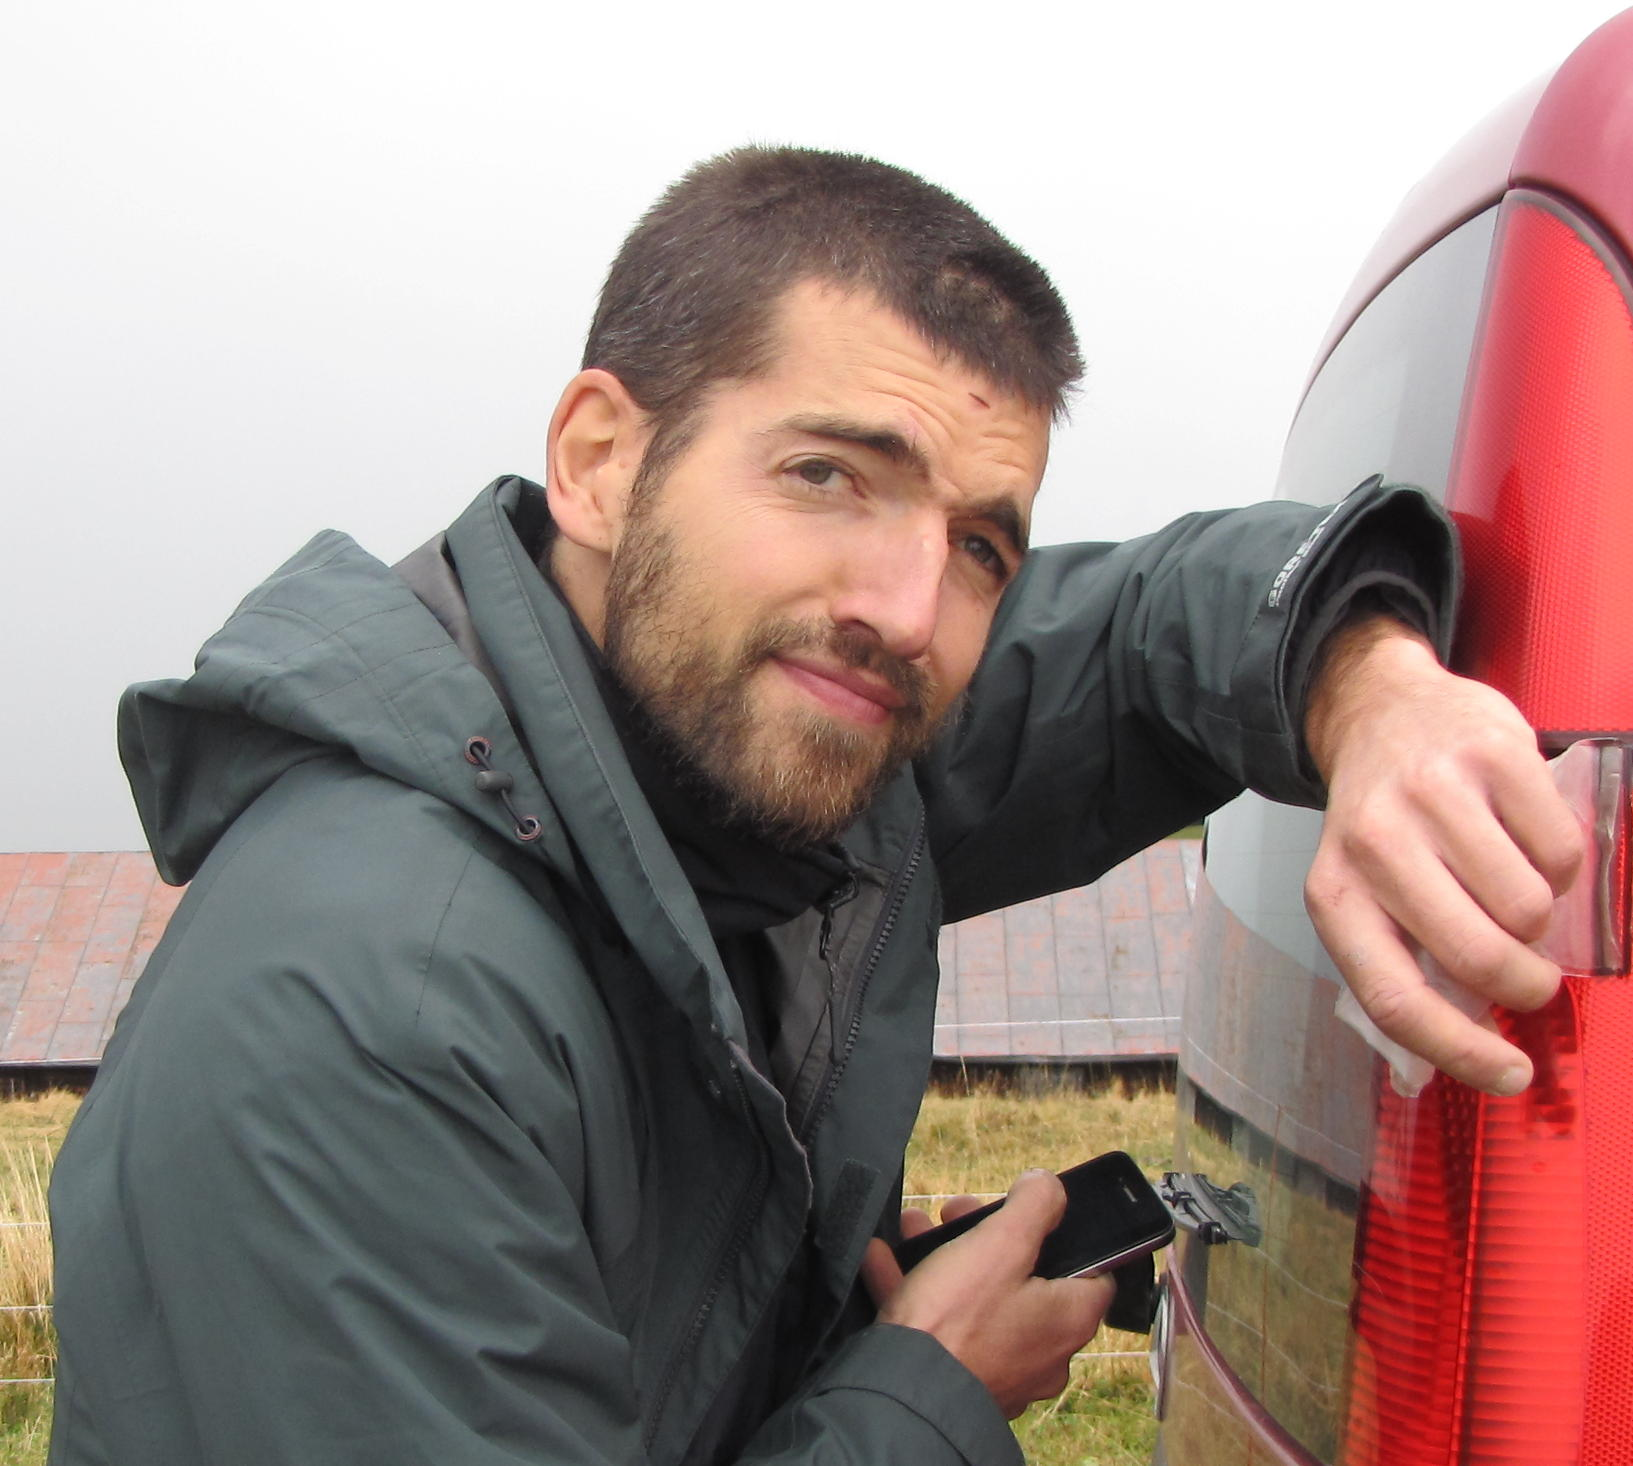
\includegraphics[width = 0.22 \textwidth]{Figures/Glauco}};}
				\uncover<5->{\node (ursina) at ($(glauco)+(1.2,0)$) {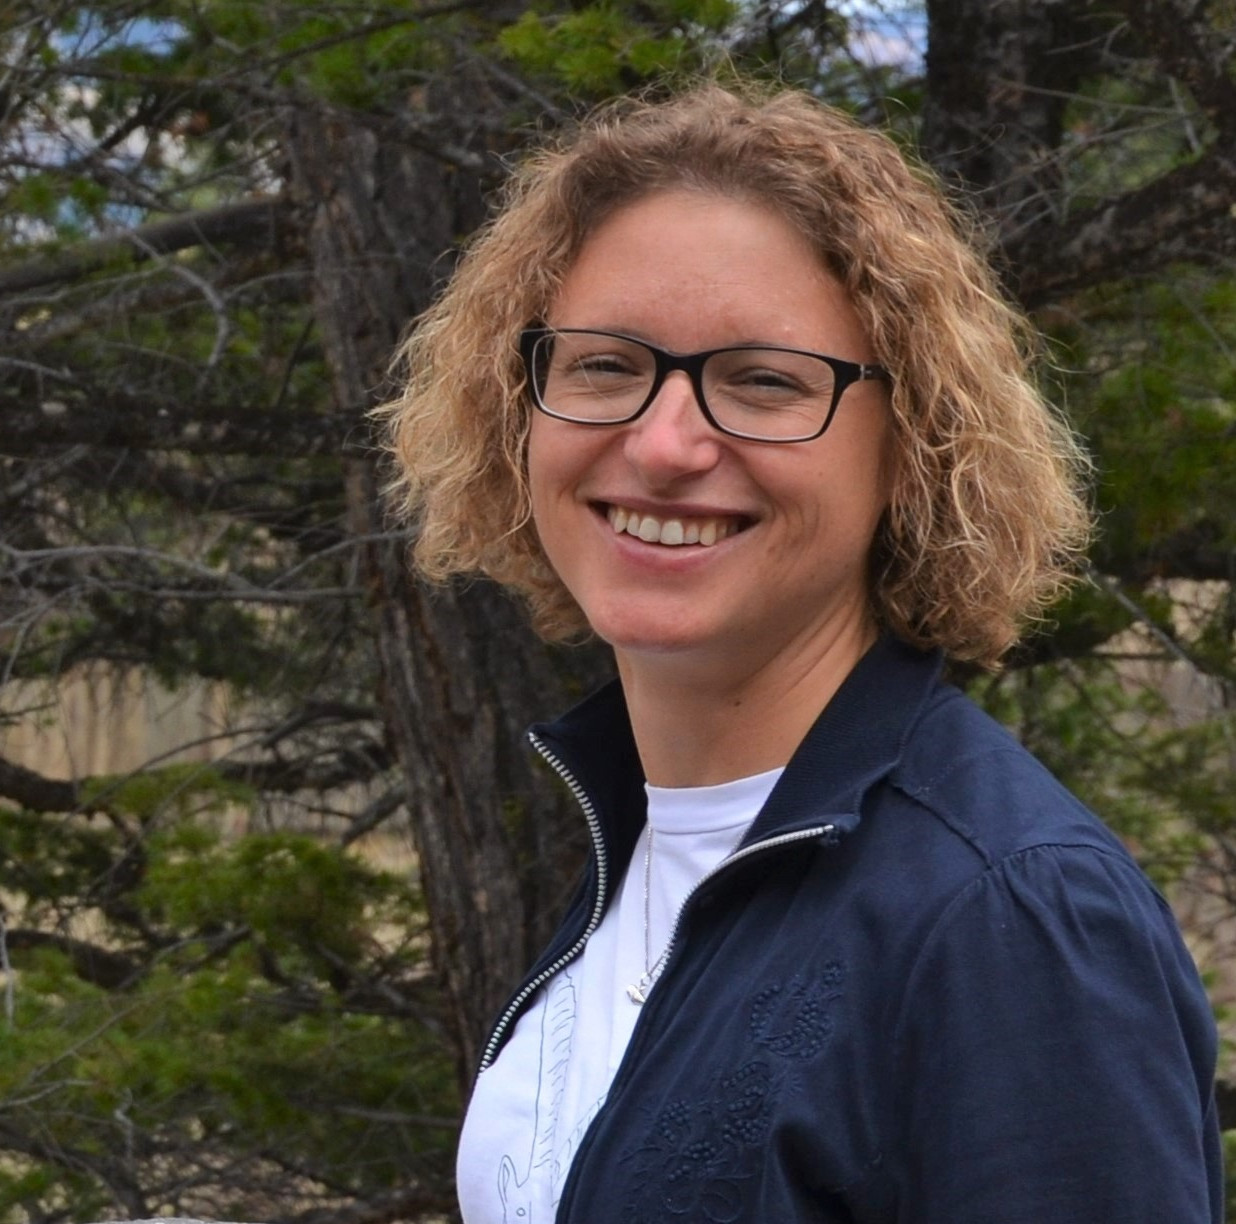
\includegraphics[width = 0.20 \textwidth]{Figures/Ursina}};}
				\uncover<6->{\node (domi) at ($(ursina)+(1.4,0)$) {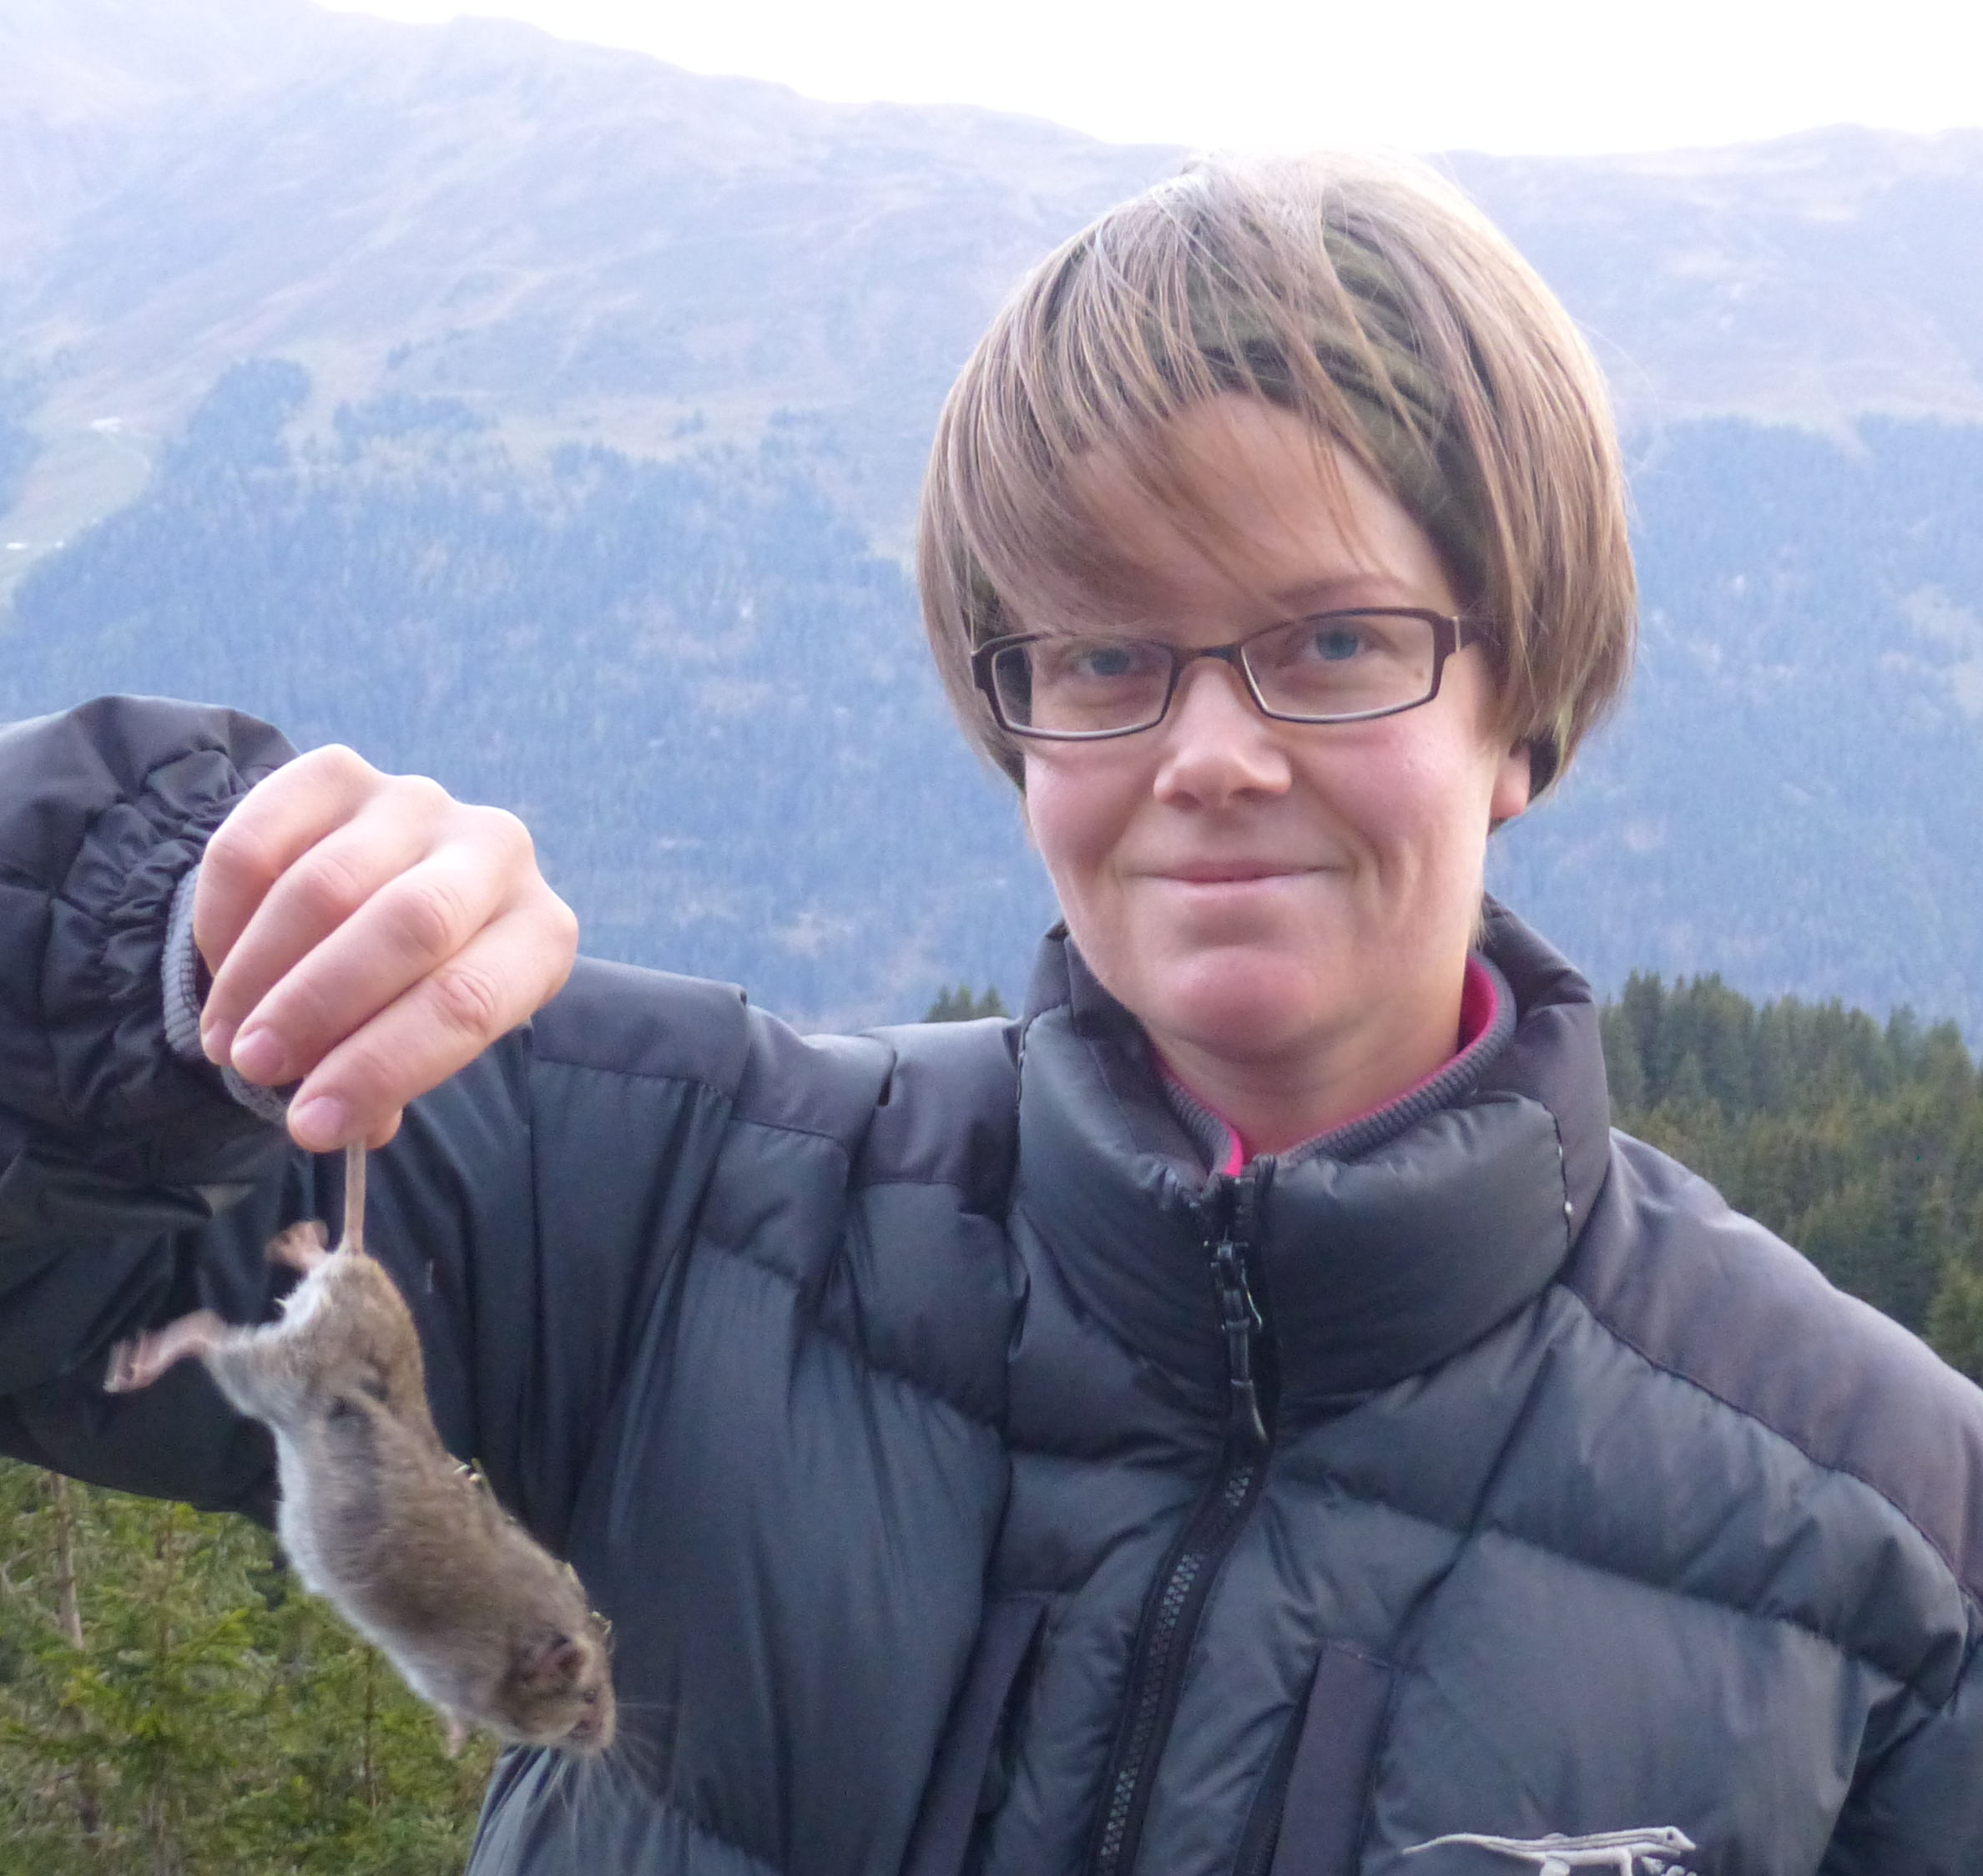
\includegraphics[width = 0.20 \textwidth]{Figures/Domi}};}
				\uncover<6->{\node (martina) at ($(domi)+(1.2,0)$) {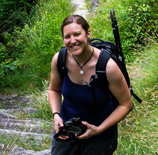
\includegraphics[width = 0.17 \textwidth]{Figures/Martina}};}
				\uncover<6->{\node (vicente) at ($(martina)+(1.2,-0.2)$) {\includegraphics[width = 0.16 \textwidth]{Figures/Vicente}};}
				\uncover<7->{\node (andres) at ($(vicente)+(1.2,-0.1)$) {\includegraphics[width = 0.2 \textwidth]{Figures/Andres}};}
				\uncover<8->{\node (koen) at ($(glauco)+(0,-1.4)$) {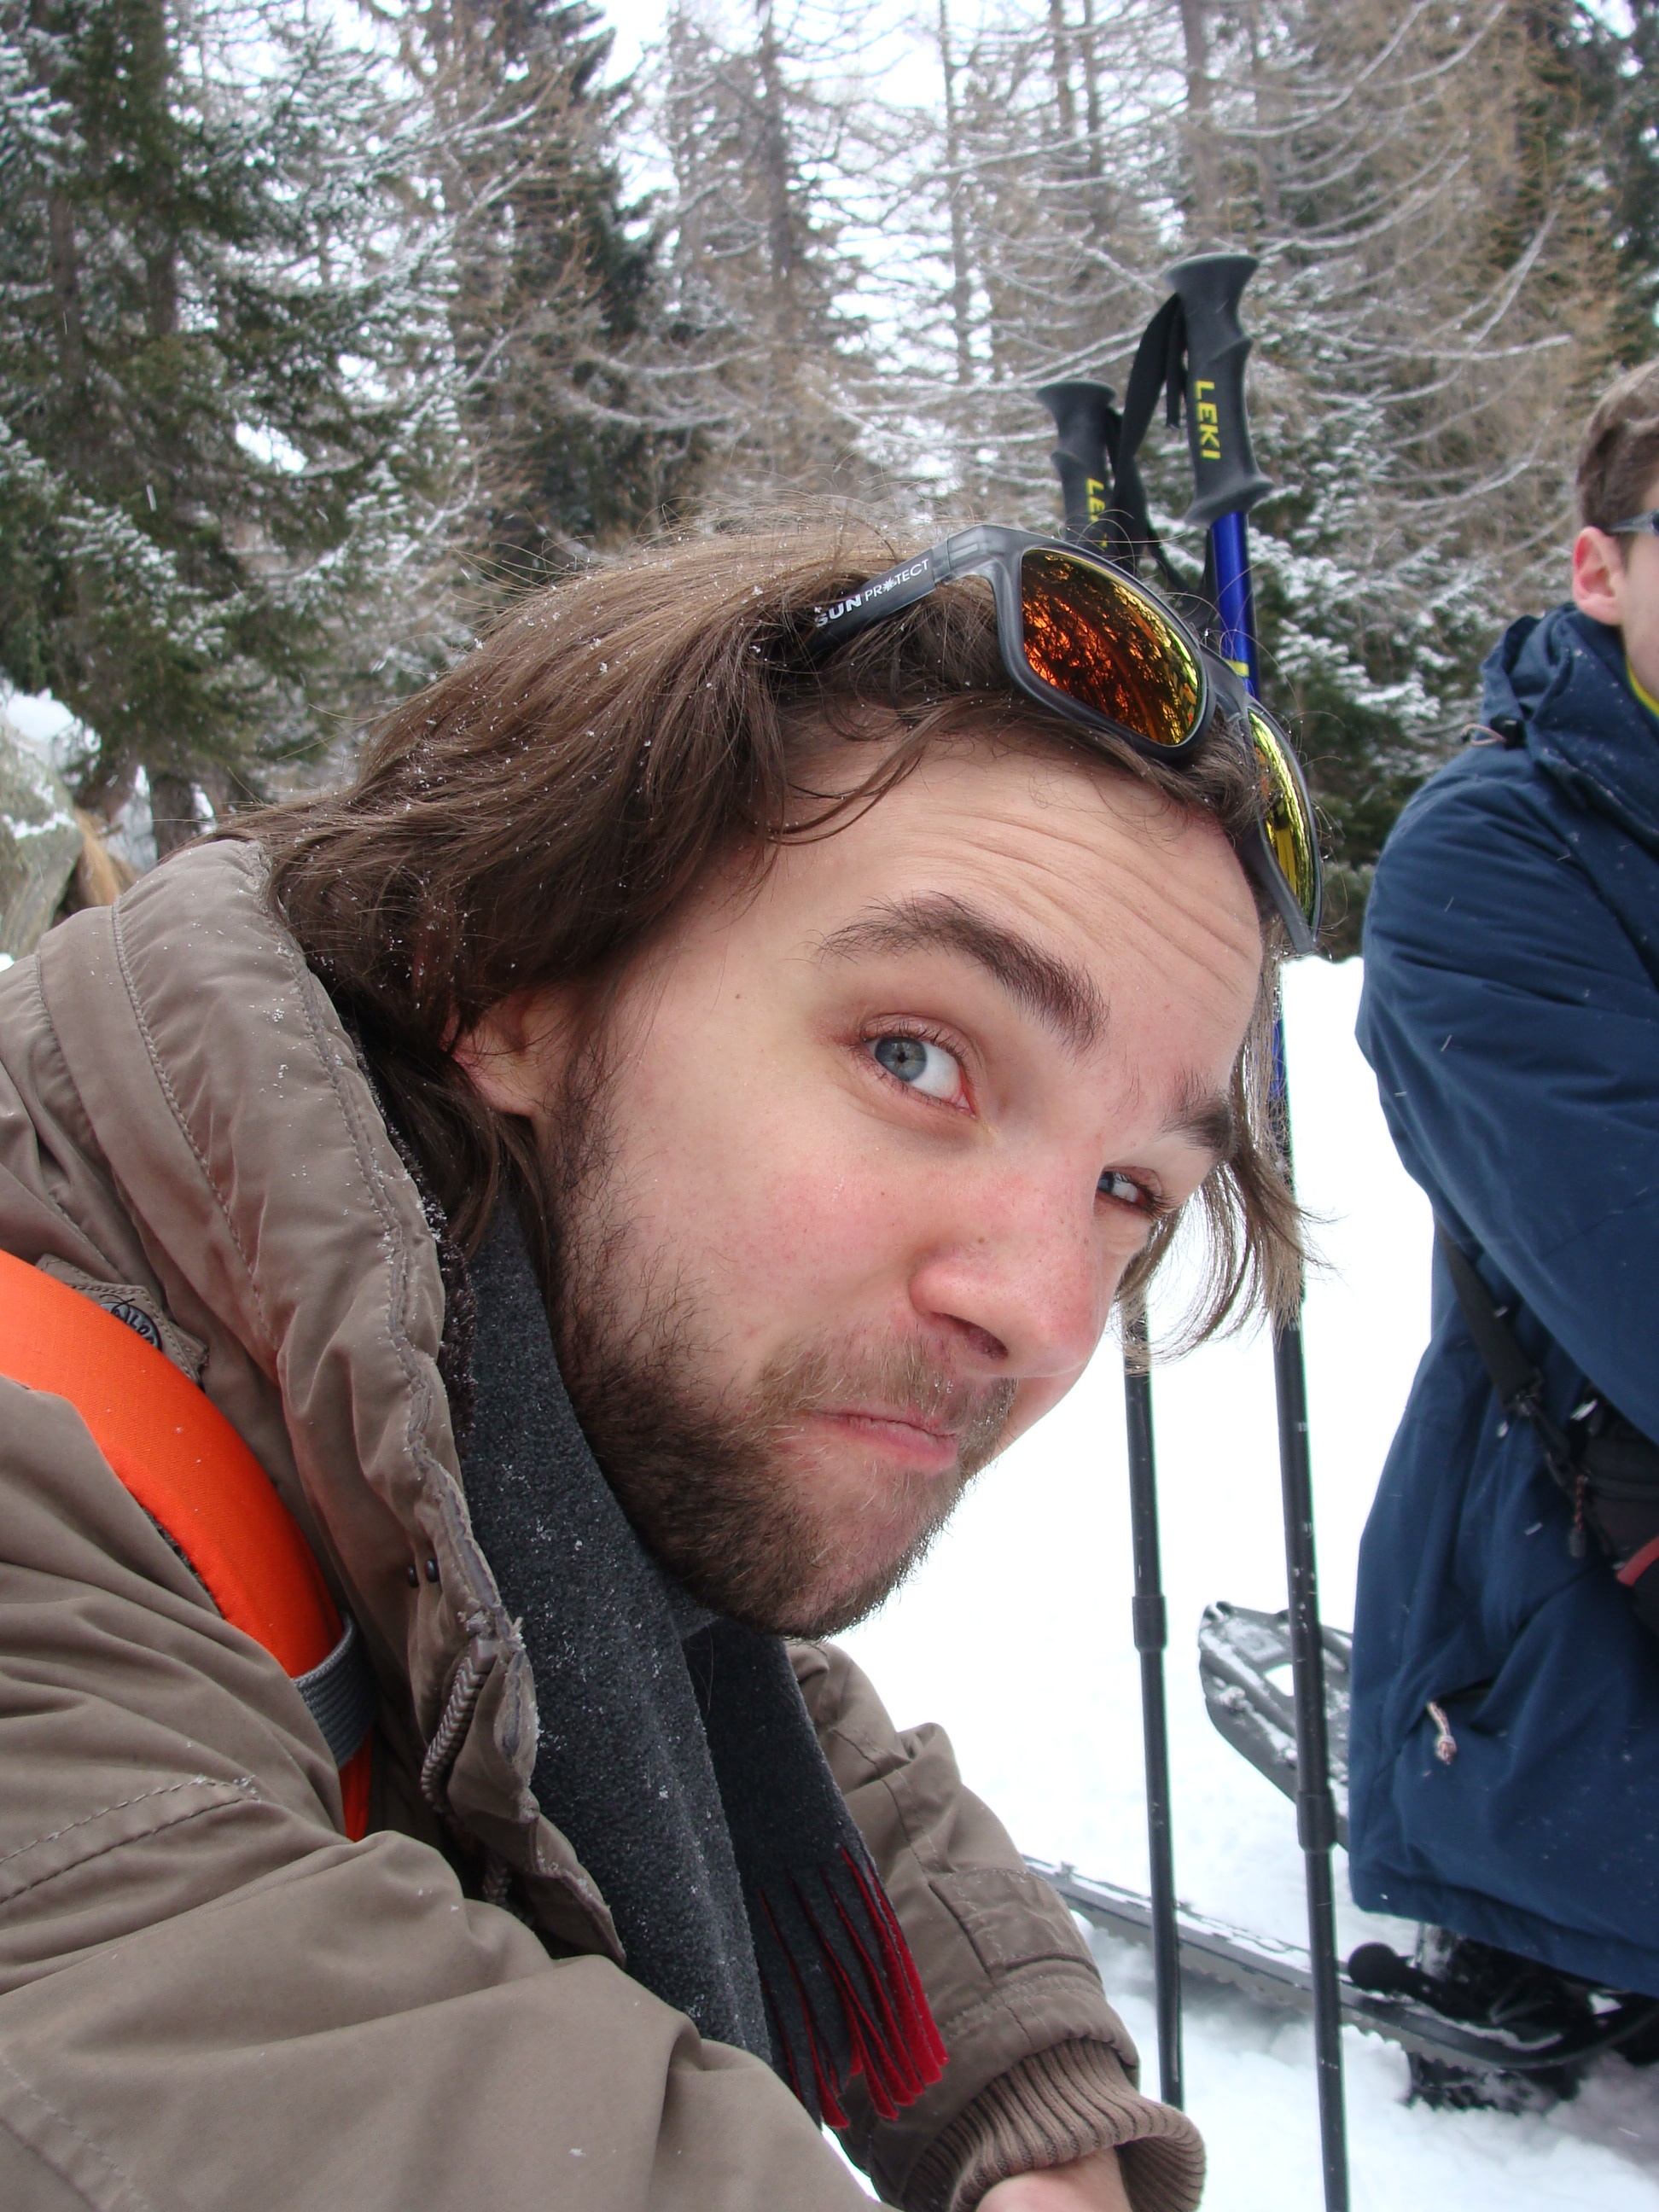
\includegraphics[width = 0.2 \textwidth]{Figures/Koen}};
				\node (marjolein) at ($(koen)+(1.2,0)$) {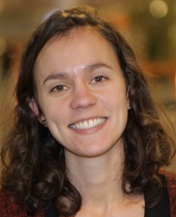
\includegraphics[width = 0.15 \textwidth]{Figures/Marjolein}};
				\node (eelke) at ($(marjolein)+(1.2,0)$) {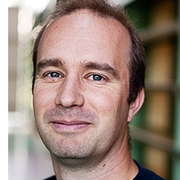
\includegraphics[width = 0.2 \textwidth]{Figures/Eelke}};
				}
				\uncover<9->{
				
				\node (philipp) at ($(eelke)+(1.2,0)$) {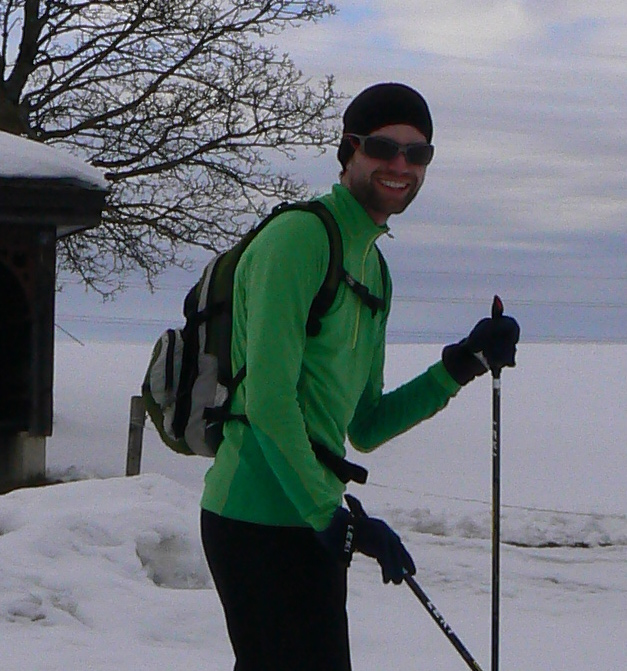
\includegraphics[width = 0.2 \textwidth]{Figures/Philipp}};
				\node (pirmin) at ($(philipp)+(1.2,0)$) {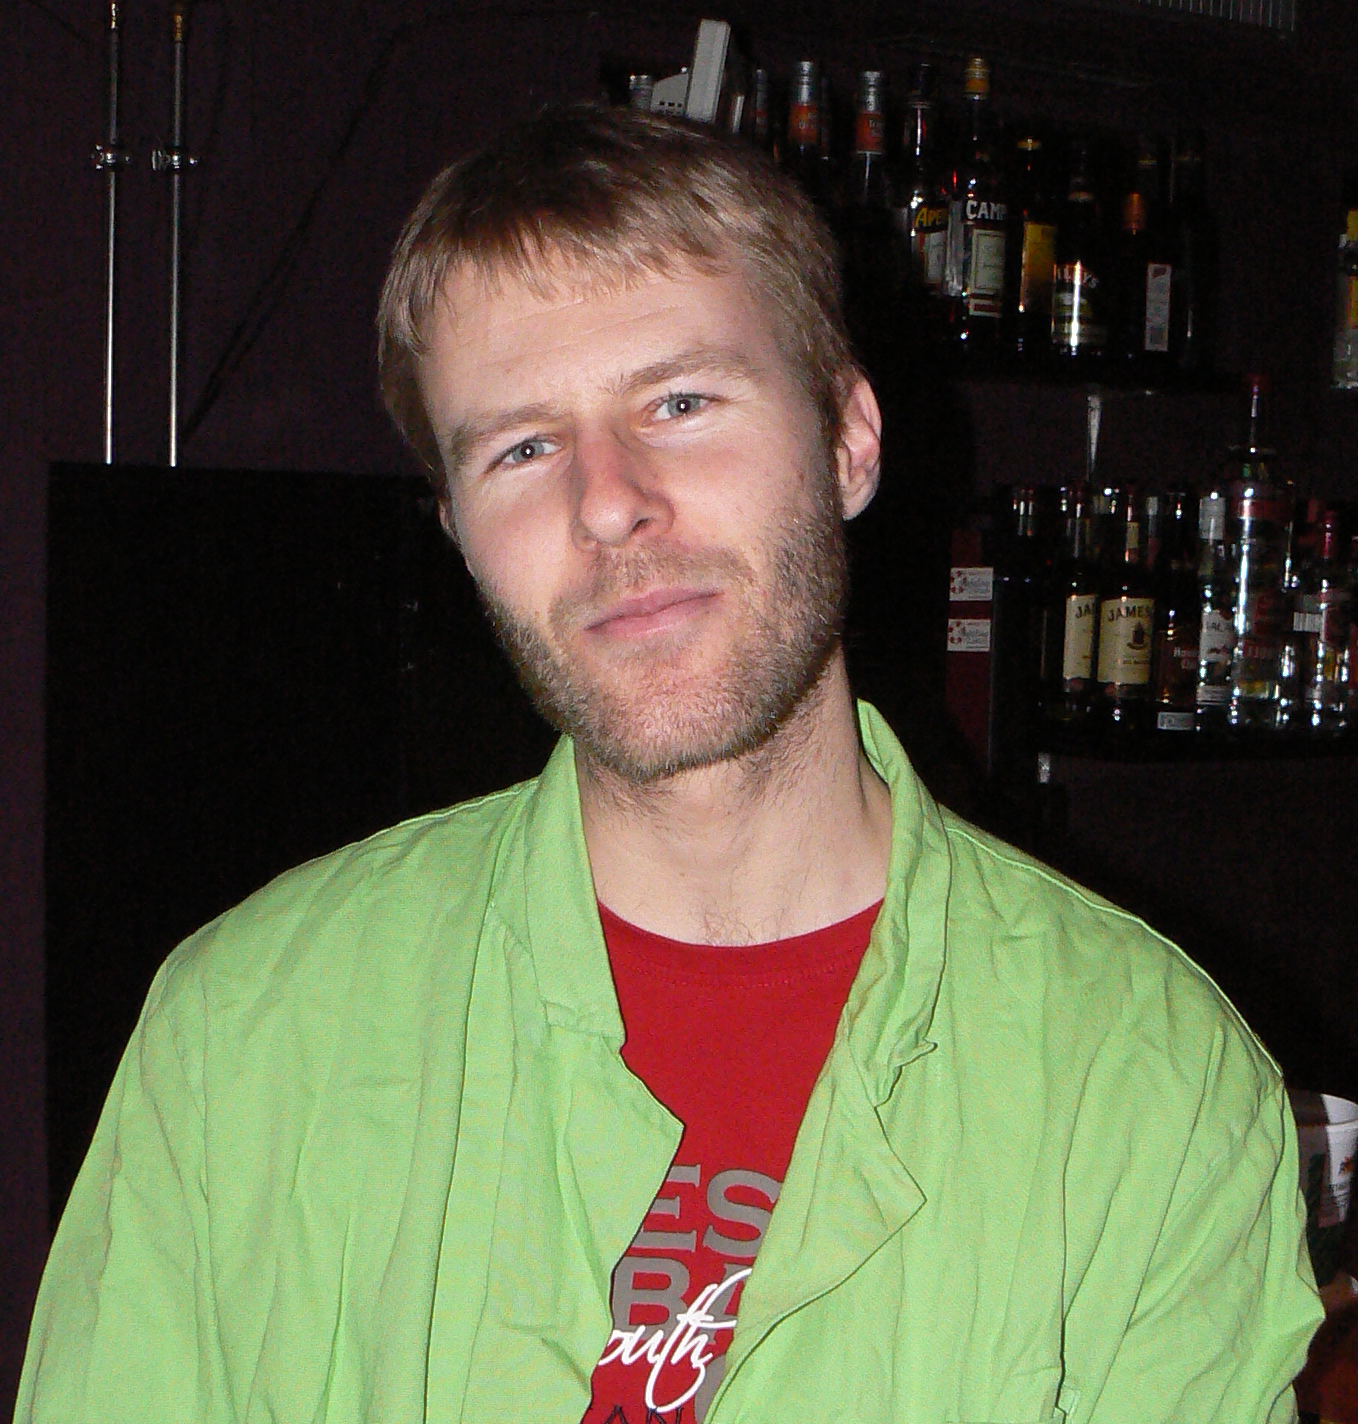
\includegraphics[width = 0.2 \textwidth]{Figures/Pirmin}};
				\node (judith) at ($(pirmin)+(1.2,0)$) {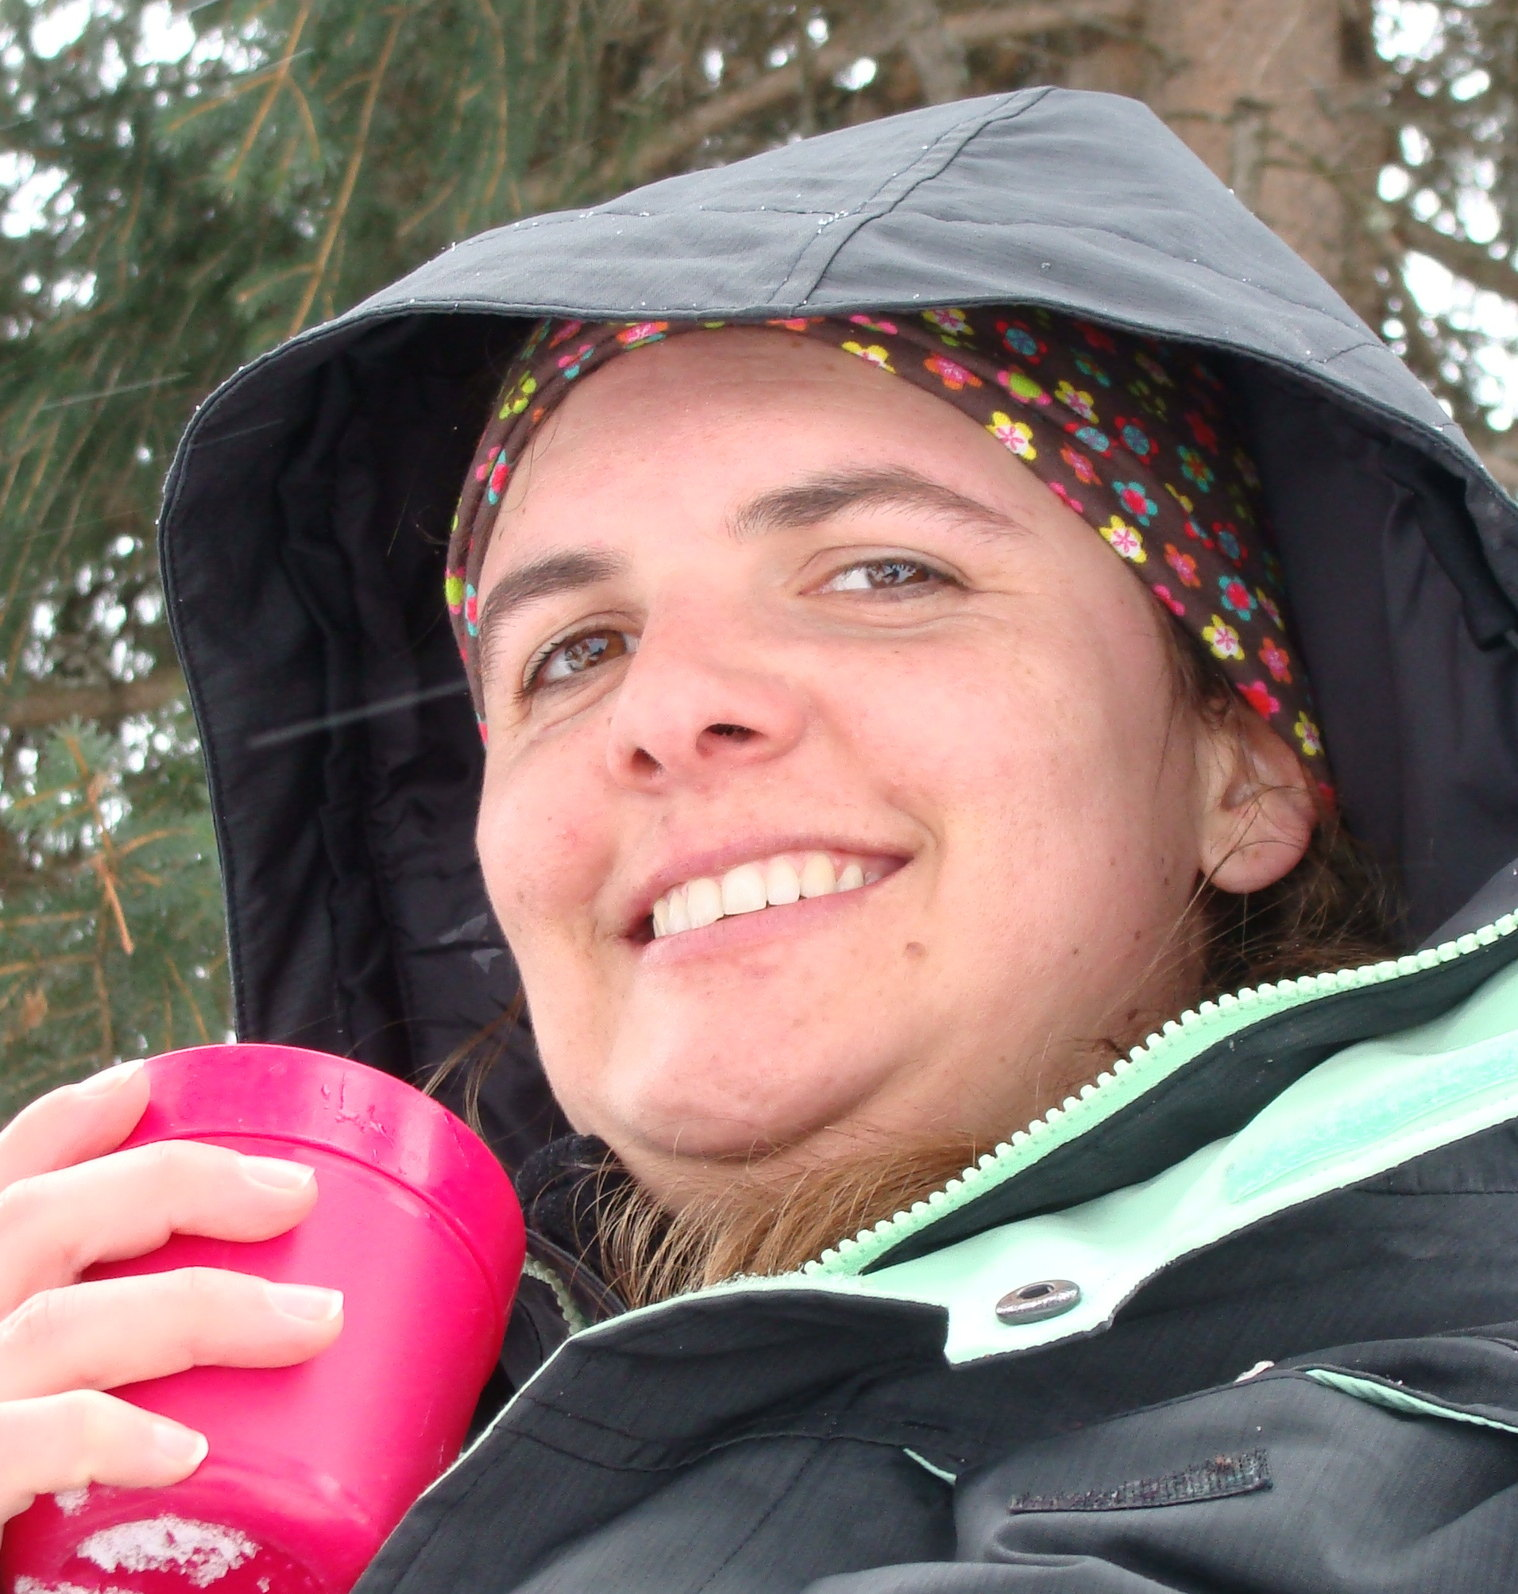
\includegraphics[width = 0.18 \textwidth]{Figures/Judith}};
				}
					\end{tikzpicture}
		\end{figure}
	\end{column}
\end{columns}

\end{frame}
%%%%%%%%%%%

\begin{frame}[plain]
\begin{columns}
\begin{column}[c]{0.7\textwidth}
		\begin{figure}[c]
			\begin{tikzpicture}

							\node (erik) at (0,0) {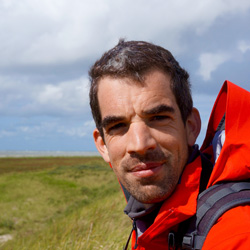
\includegraphics[width = 0.2 \textwidth]{Figures/Erik}};
				\node (lukas) at ($(erik)+(1.2,0)$) {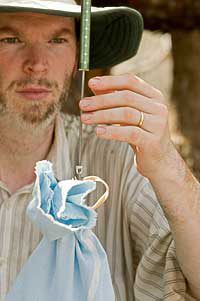
\includegraphics[width = 0.15 \textwidth]{Figures/Lukas}};
				\node (barbara) at ($(lukas)+(1,0)$) {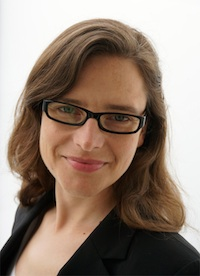
\includegraphics[width = 0.15 \textwidth]{Figures/Barbara}};
				\node (arpat) at ($(barbara)+(1.3,0)$) {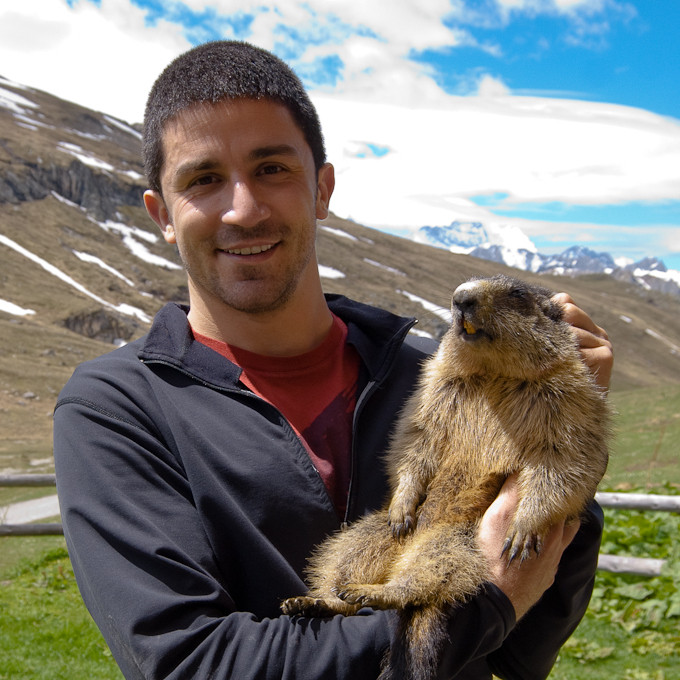
\includegraphics[width = 0.2 \textwidth]{Figures/Arpat}};
				\node (marc) at ($(arpat)+(1.2,0)$) {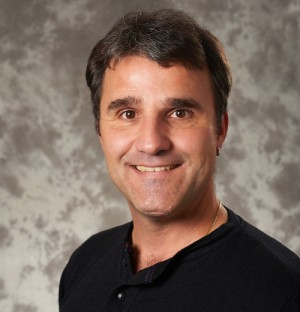
\includegraphics[width = 0.2 \textwidth]{Figures/Marc}};
				\node (jarrod) at ($(marc)+(1.3,0)$) {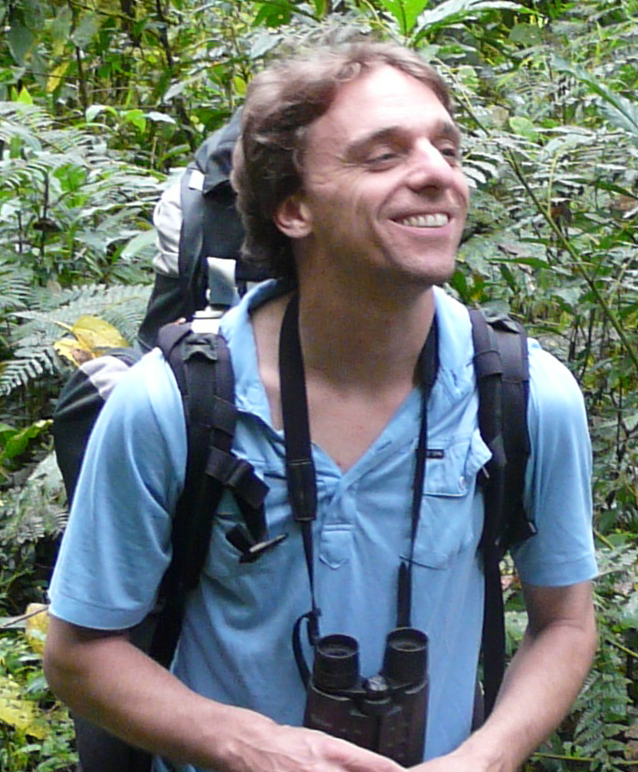
\includegraphics[width = 0.2\textwidth]{Figures/Jarrod}};
				\node (glauco) at ($(erik)+(0,-1.4)$) {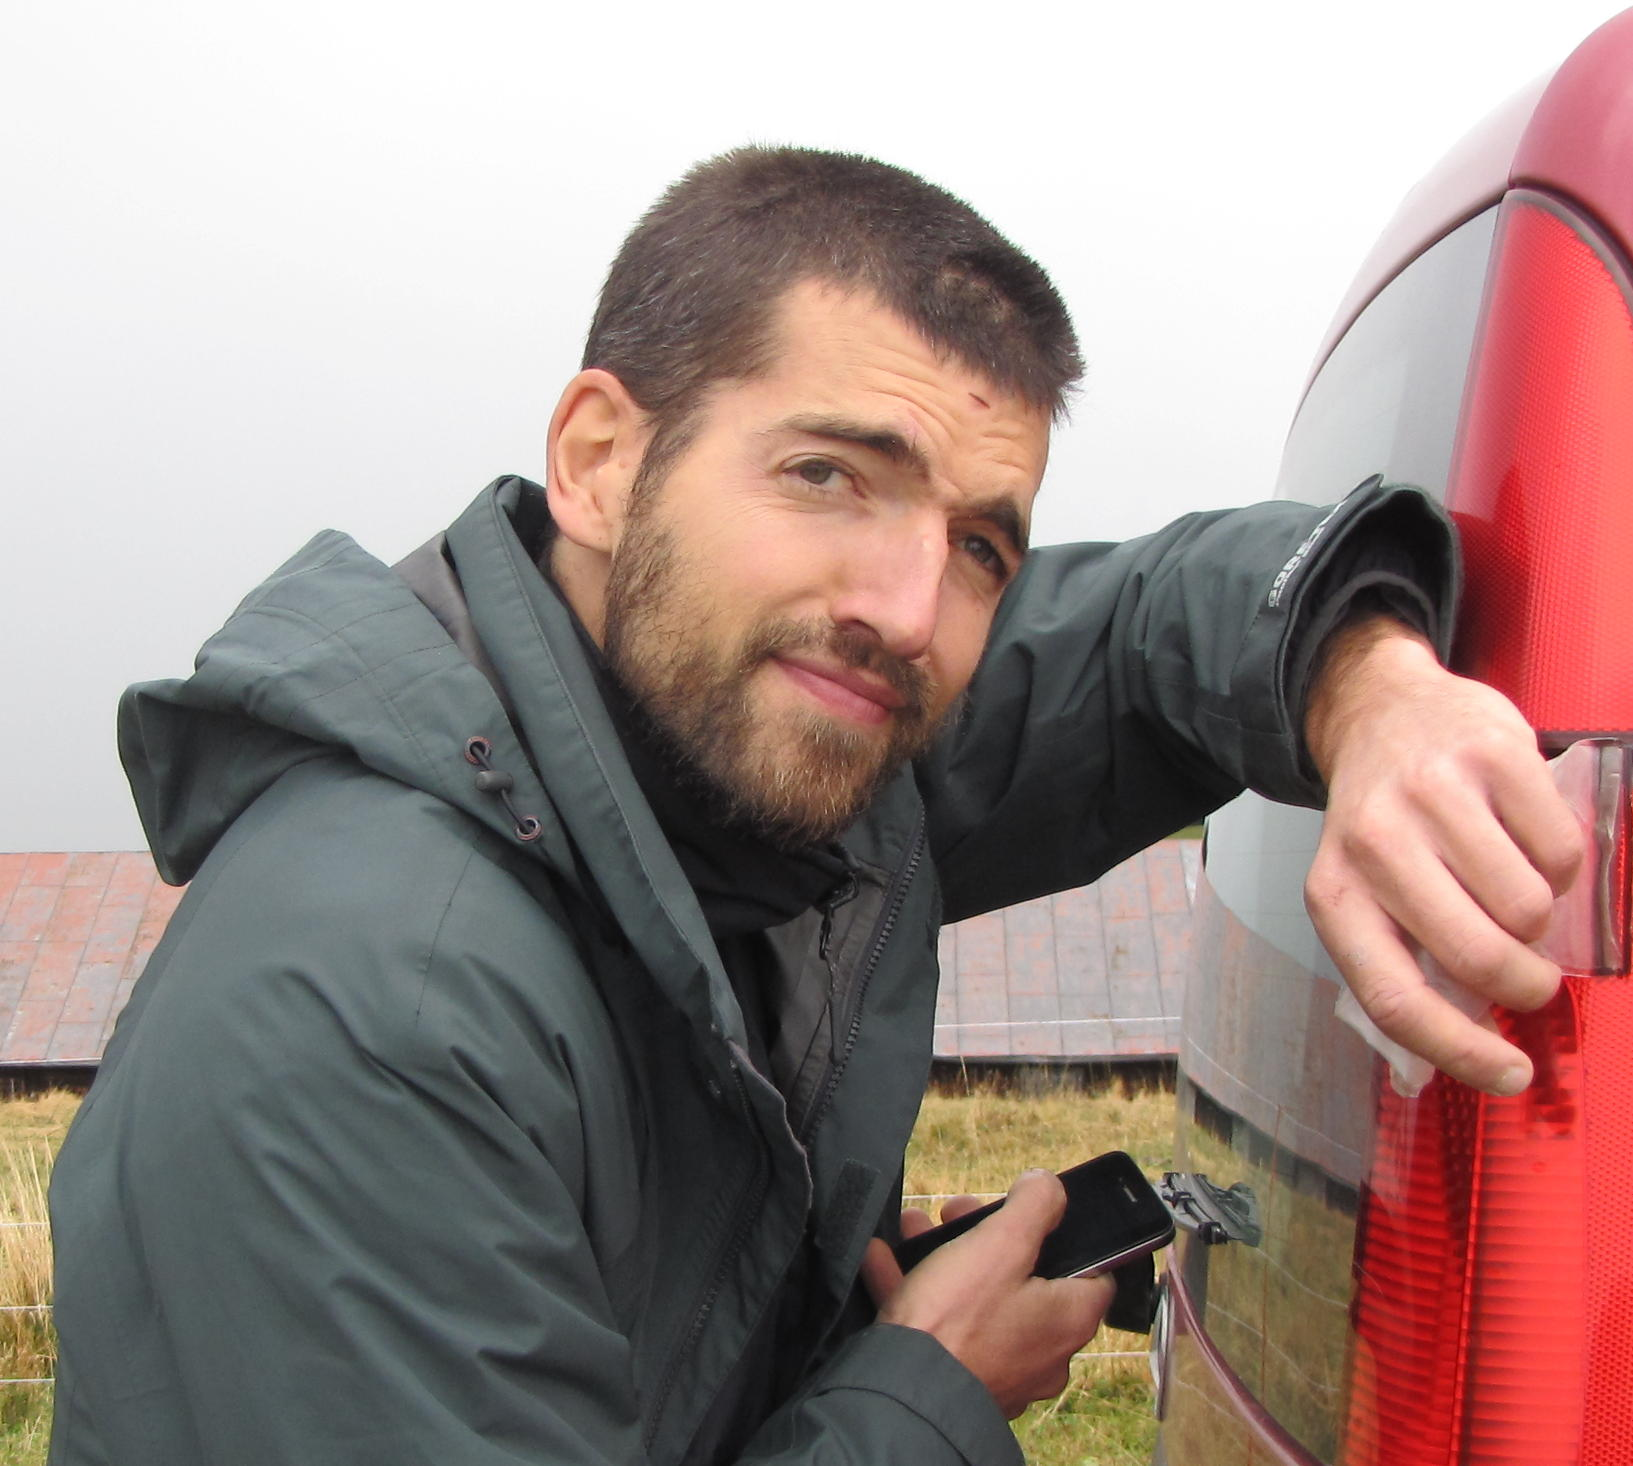
\includegraphics[width = 0.22 \textwidth]{Figures/Glauco}};
			\node (ursina) at ($(glauco)+(1.2,0)$) {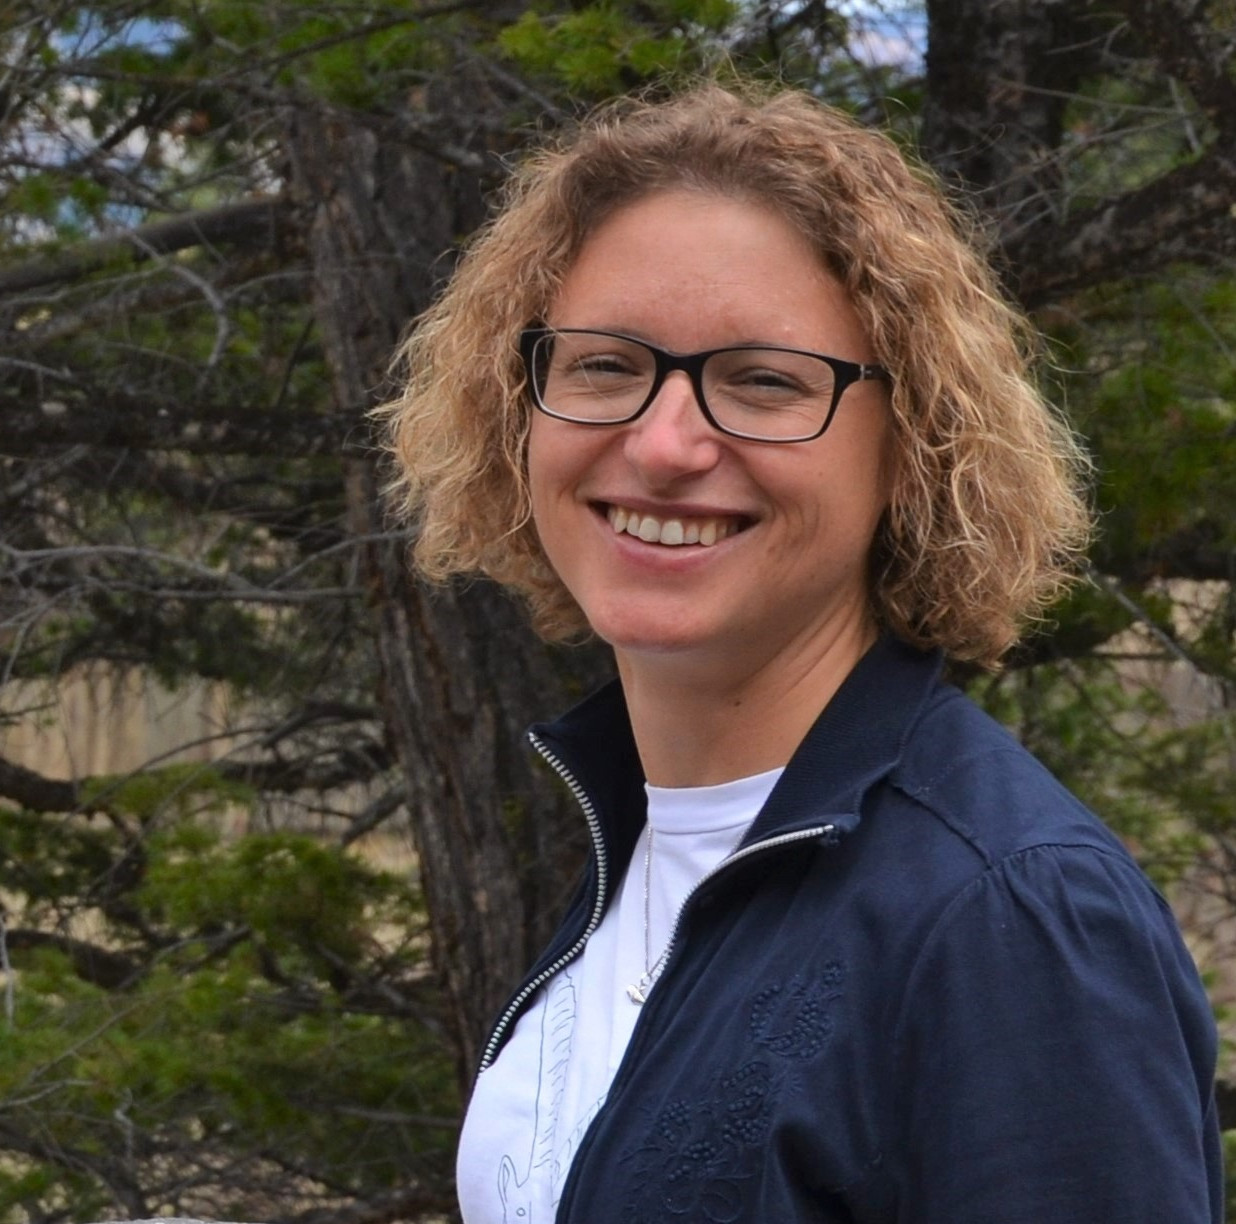
\includegraphics[width = 0.20 \textwidth]{Figures/Ursina}};
				\node (domi) at ($(ursina)+(1.4,0)$) {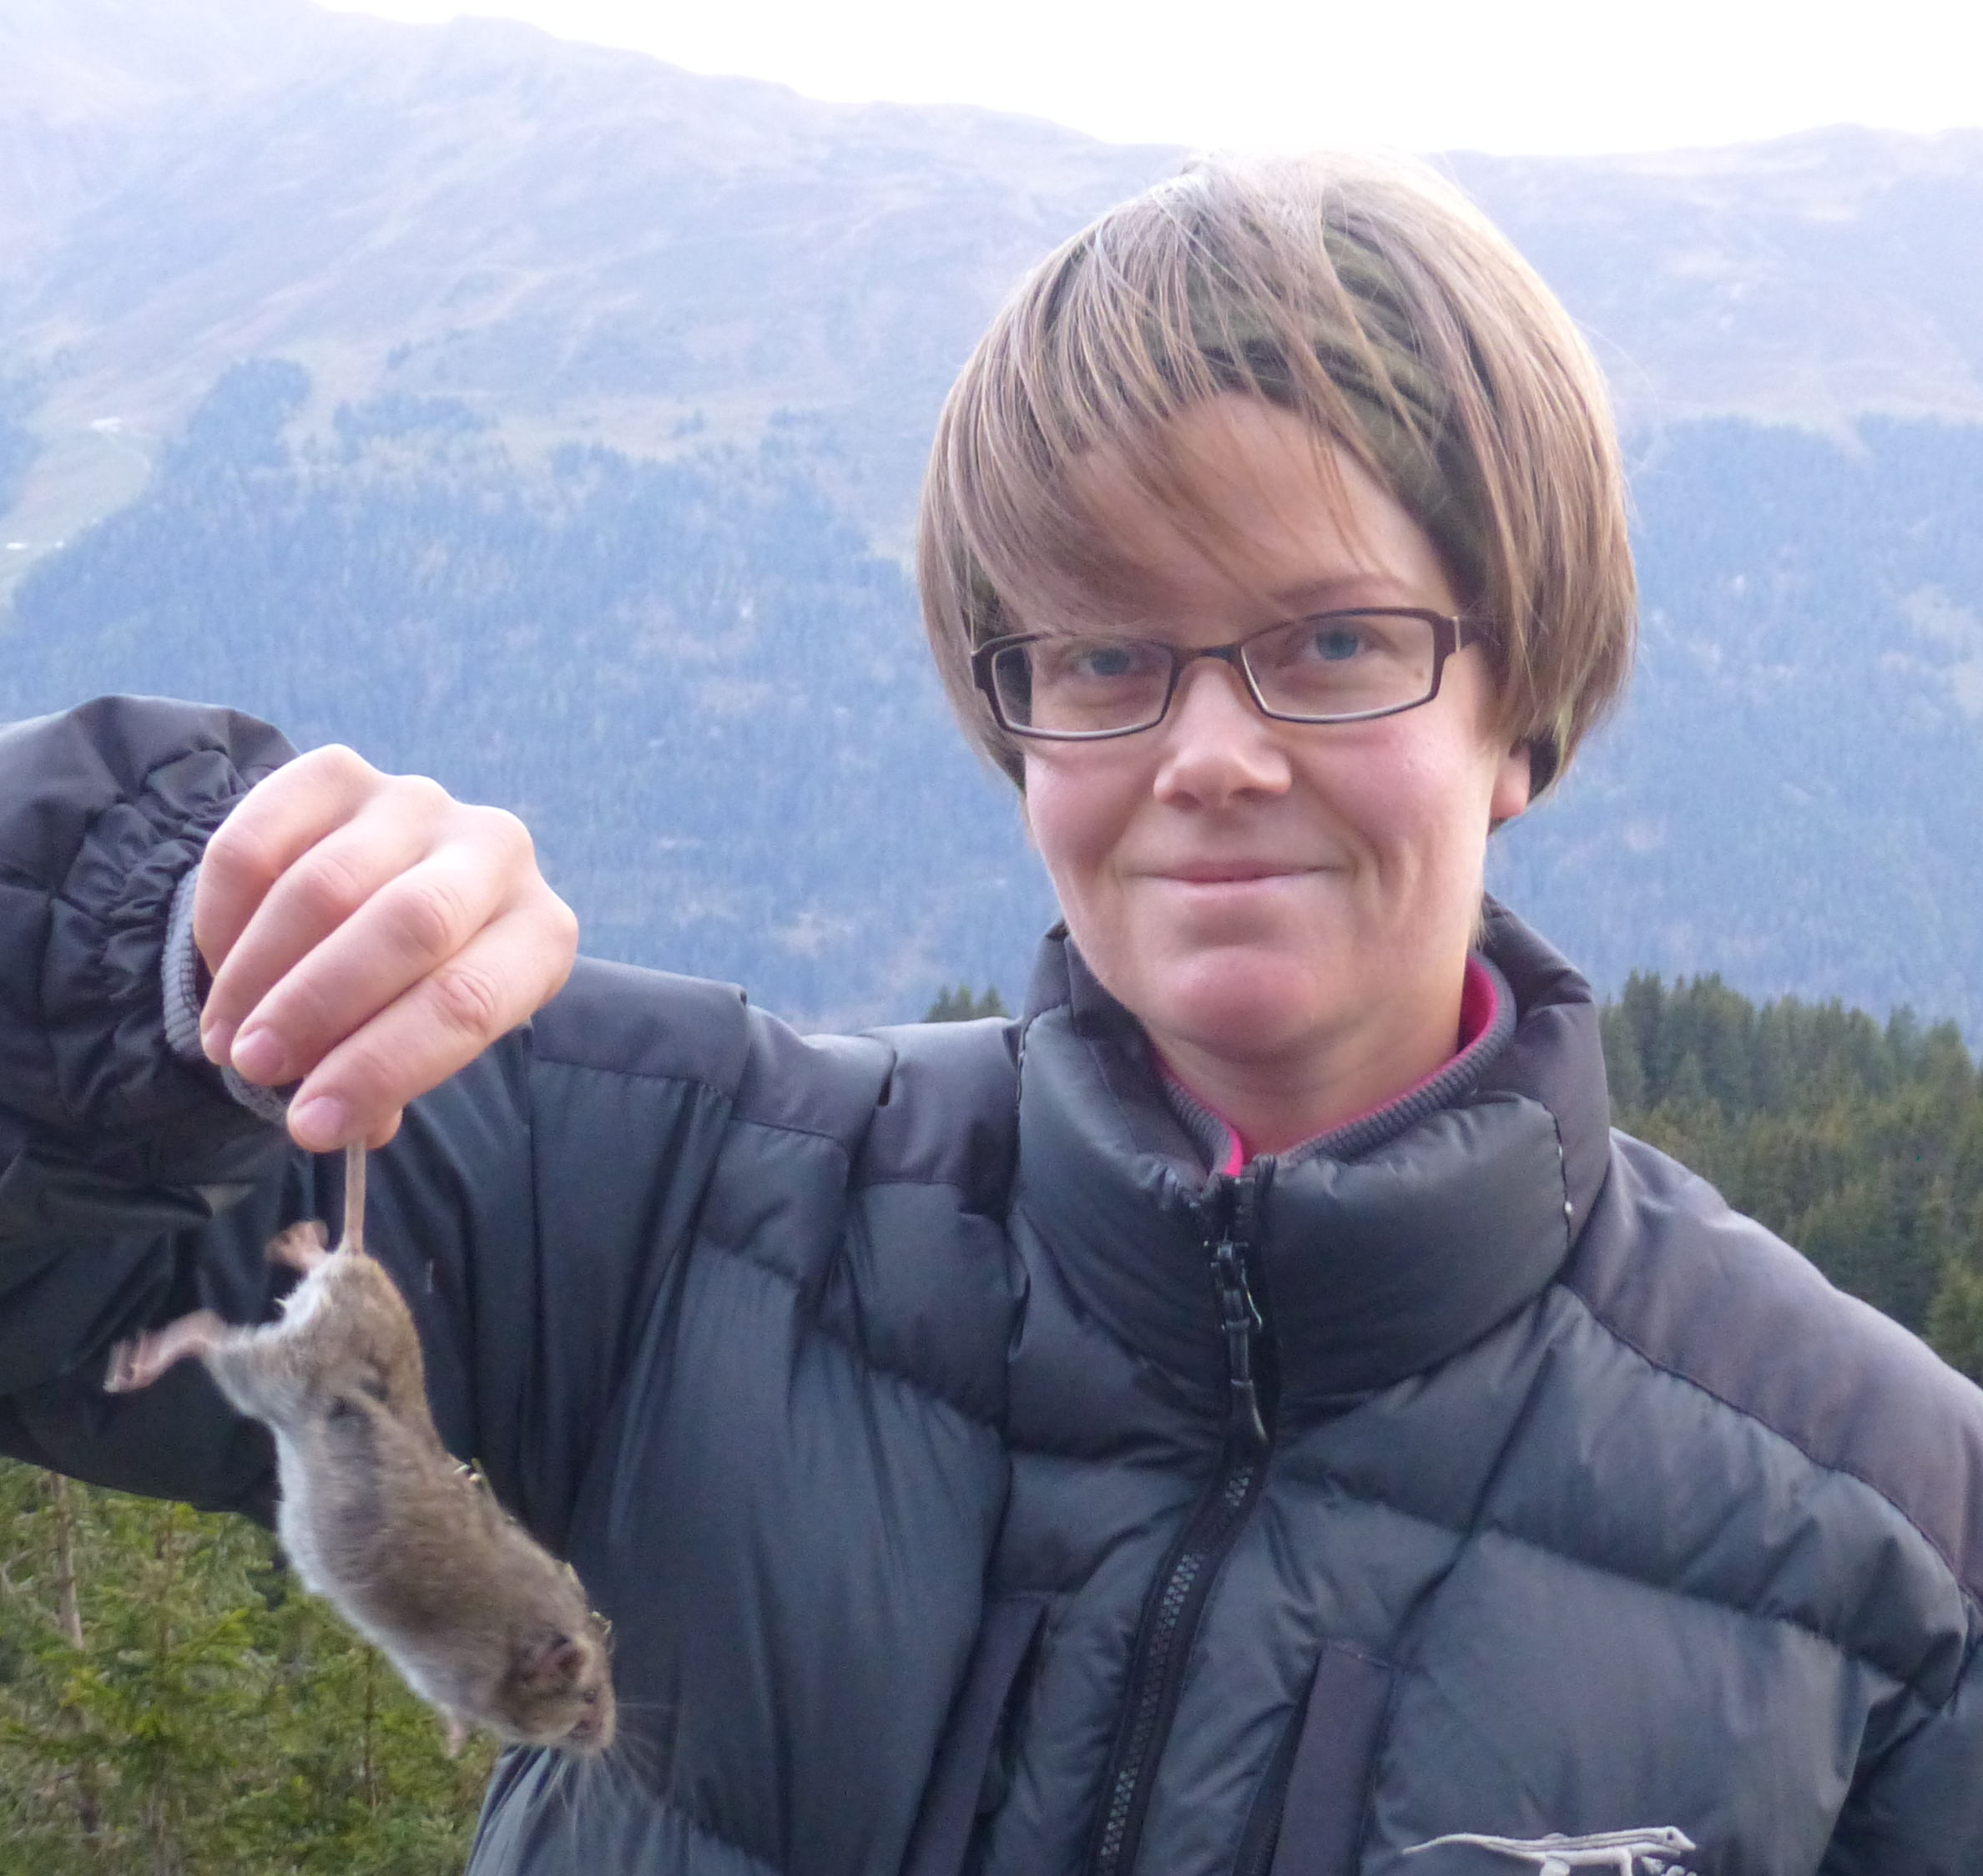
\includegraphics[width = 0.20 \textwidth]{Figures/Domi}};
				\node (martina) at ($(domi)+(1.2,0)$) {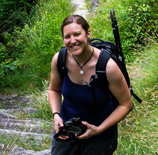
\includegraphics[width = 0.17 \textwidth]{Figures/Martina}};
\node (vicente) at ($(martina)+(1.2,-0.2)$) {\includegraphics[width = 0.16 \textwidth]{Figures/Vicente}};
	\node (andres) at ($(vicente)+(1.2,-0.1)$) {\includegraphics[width = 0.2 \textwidth]{Figures/Andres}};
\node (koen) at ($(glauco)+(0,-1.4)$) {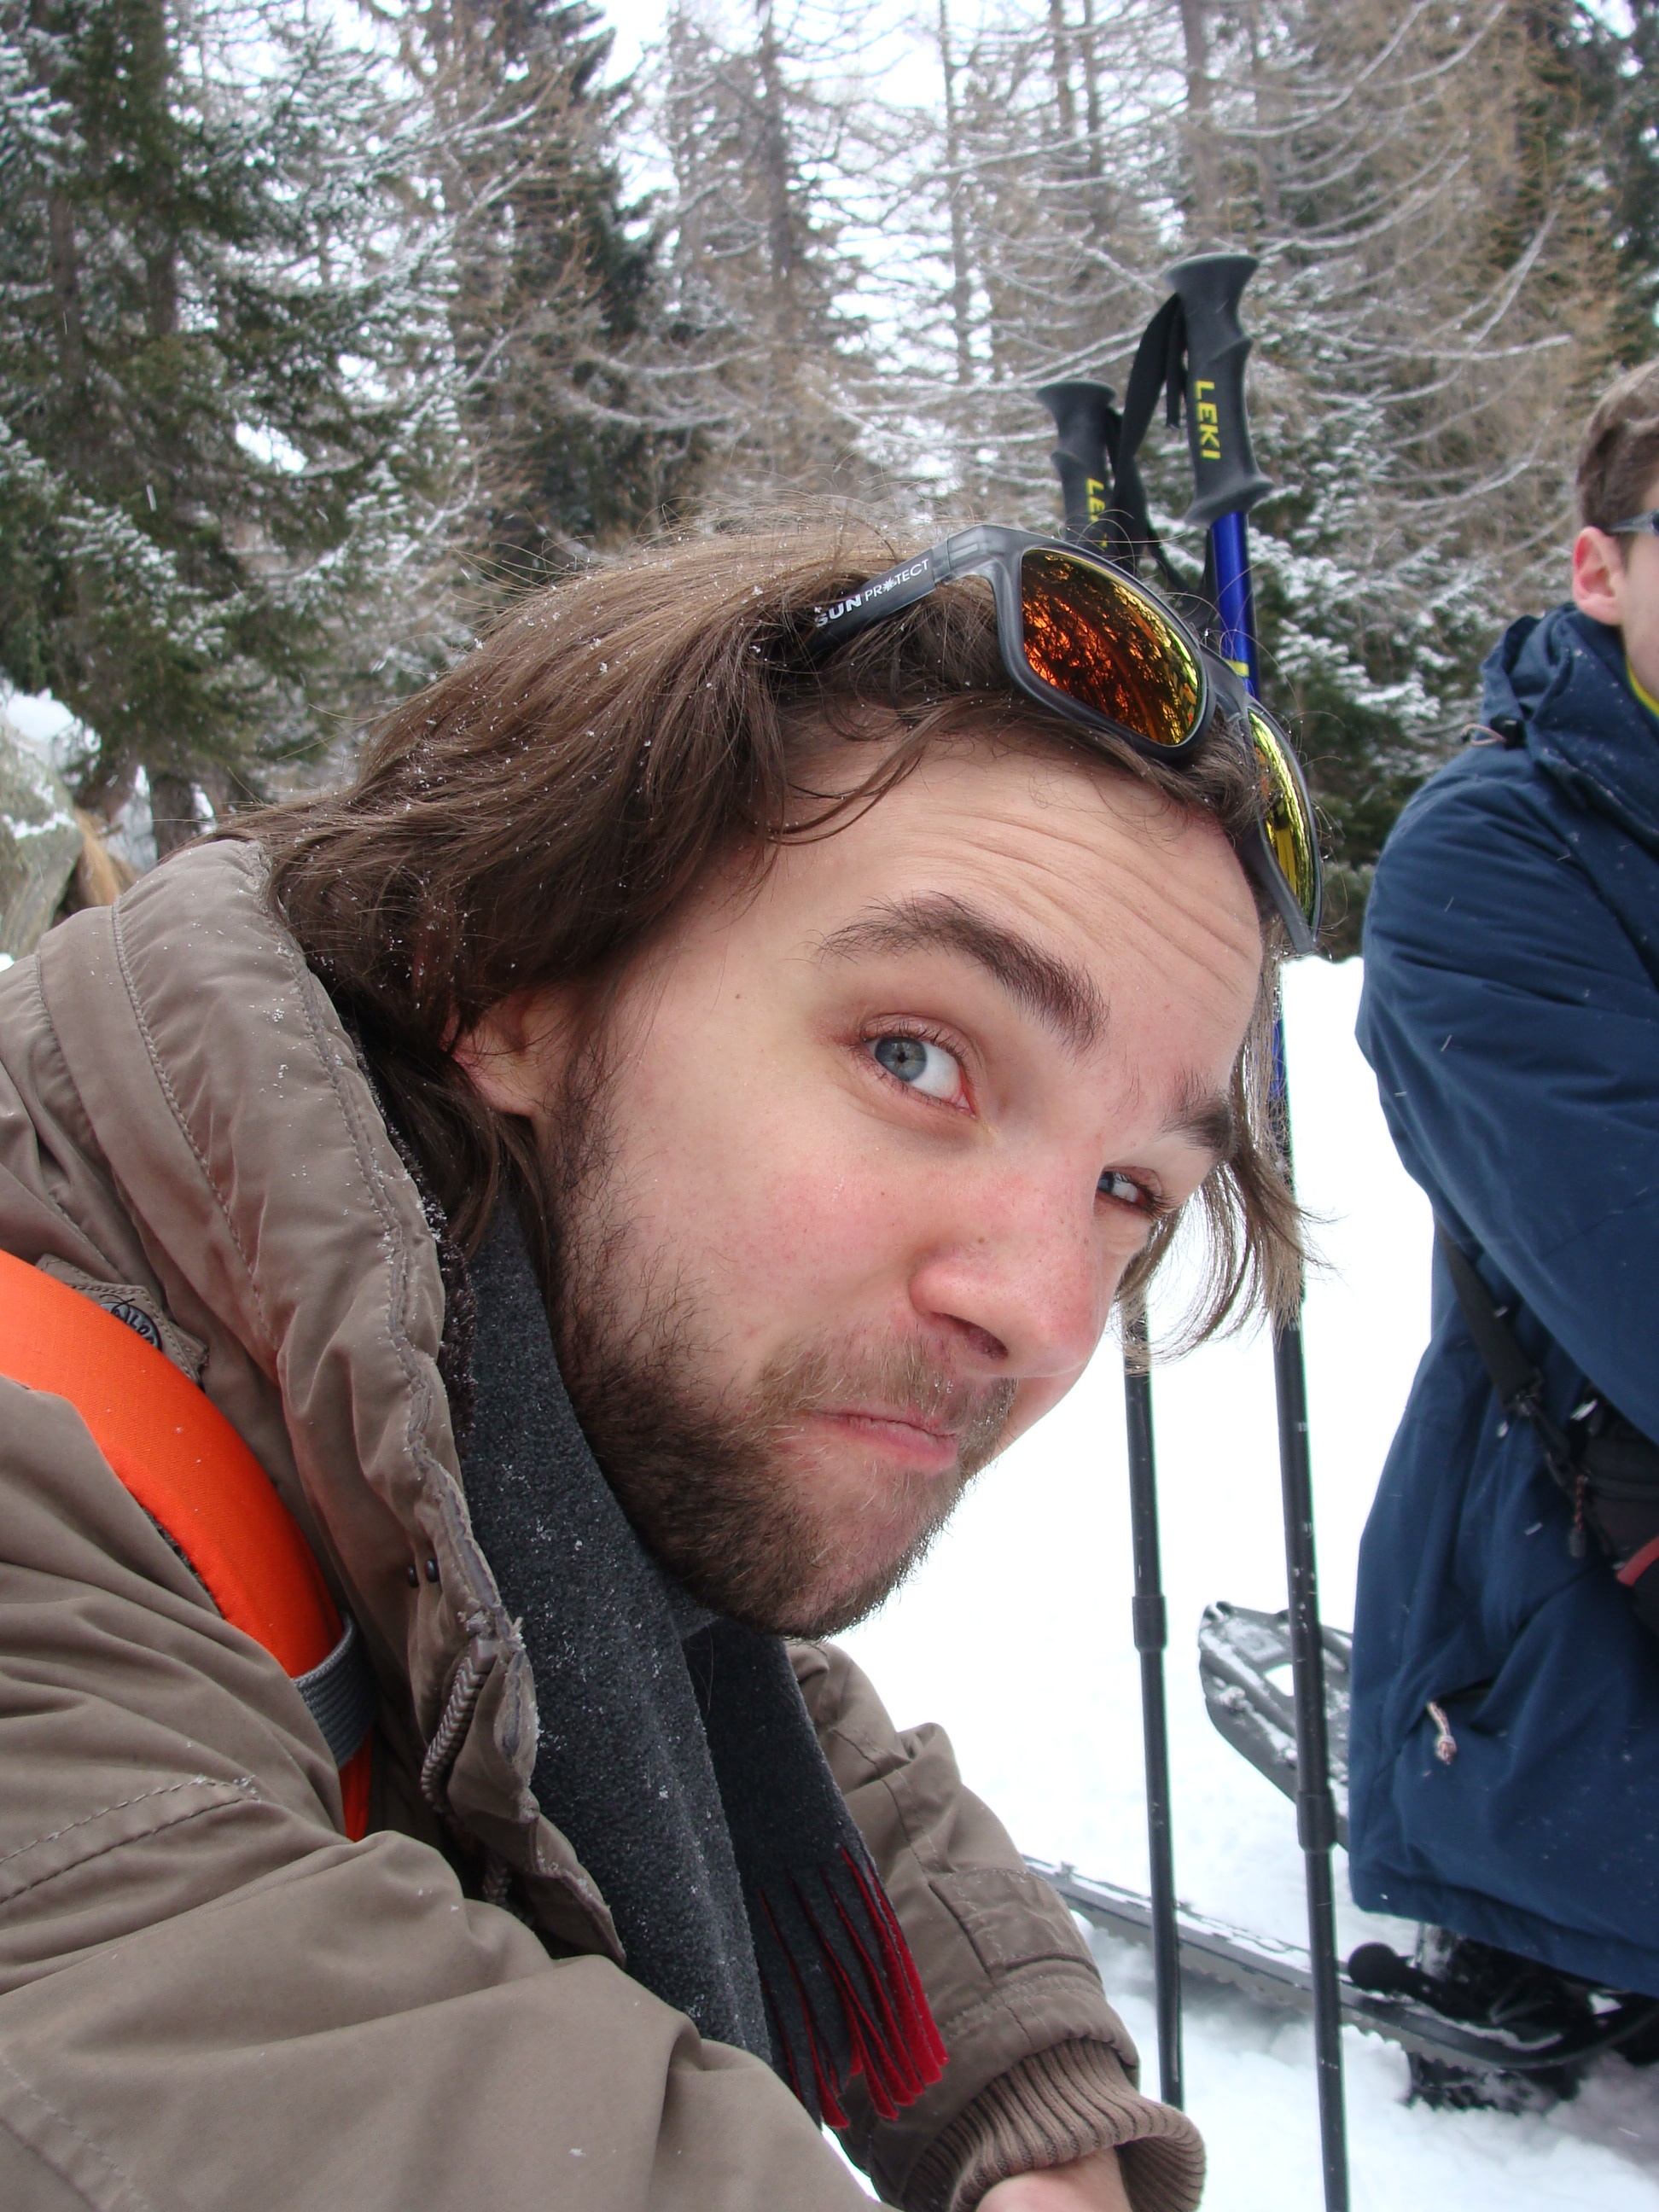
\includegraphics[width = 0.2 \textwidth]{Figures/Koen}};
				\node (marjolein) at ($(koen)+(1.2,0)$) {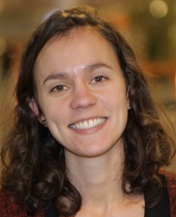
\includegraphics[width = 0.15 \textwidth]{Figures/Marjolein}};
				\node (eelke) at ($(marjolein)+(1.2,0)$) {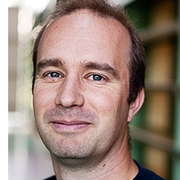
\includegraphics[width = 0.2 \textwidth]{Figures/Eelke}};
				
				
				\node (philipp) at ($(eelke)+(1.2,0)$) {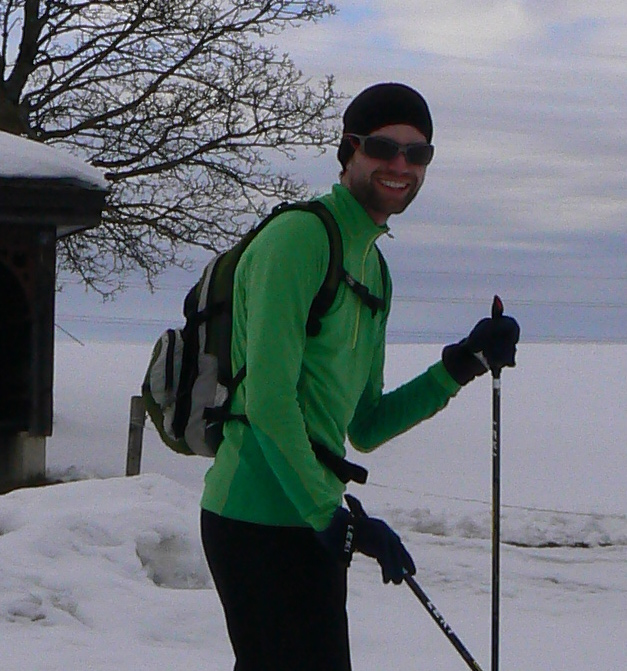
\includegraphics[width = 0.2 \textwidth]{Figures/Philipp}};
				\node (pirmin) at ($(philipp)+(1.2,0)$) {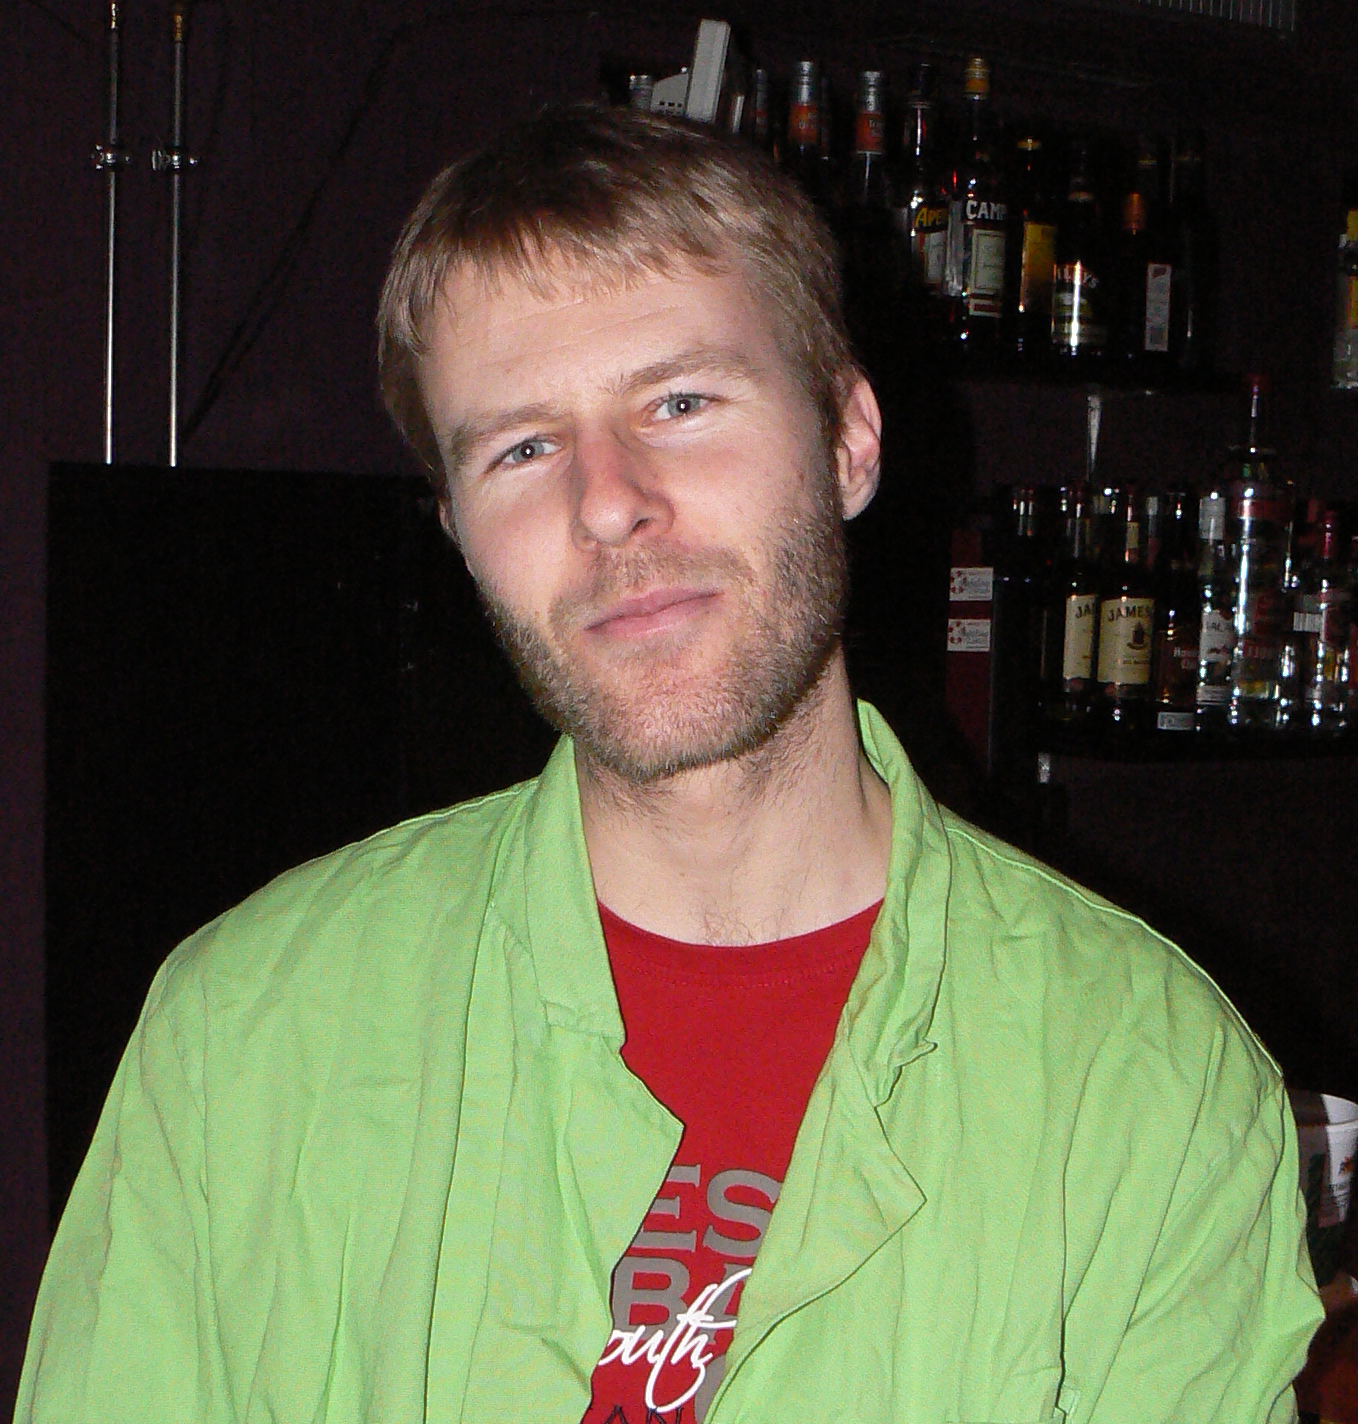
\includegraphics[width = 0.2 \textwidth]{Figures/Pirmin}};
				\node (judith) at ($(pirmin)+(1.2,0)$) {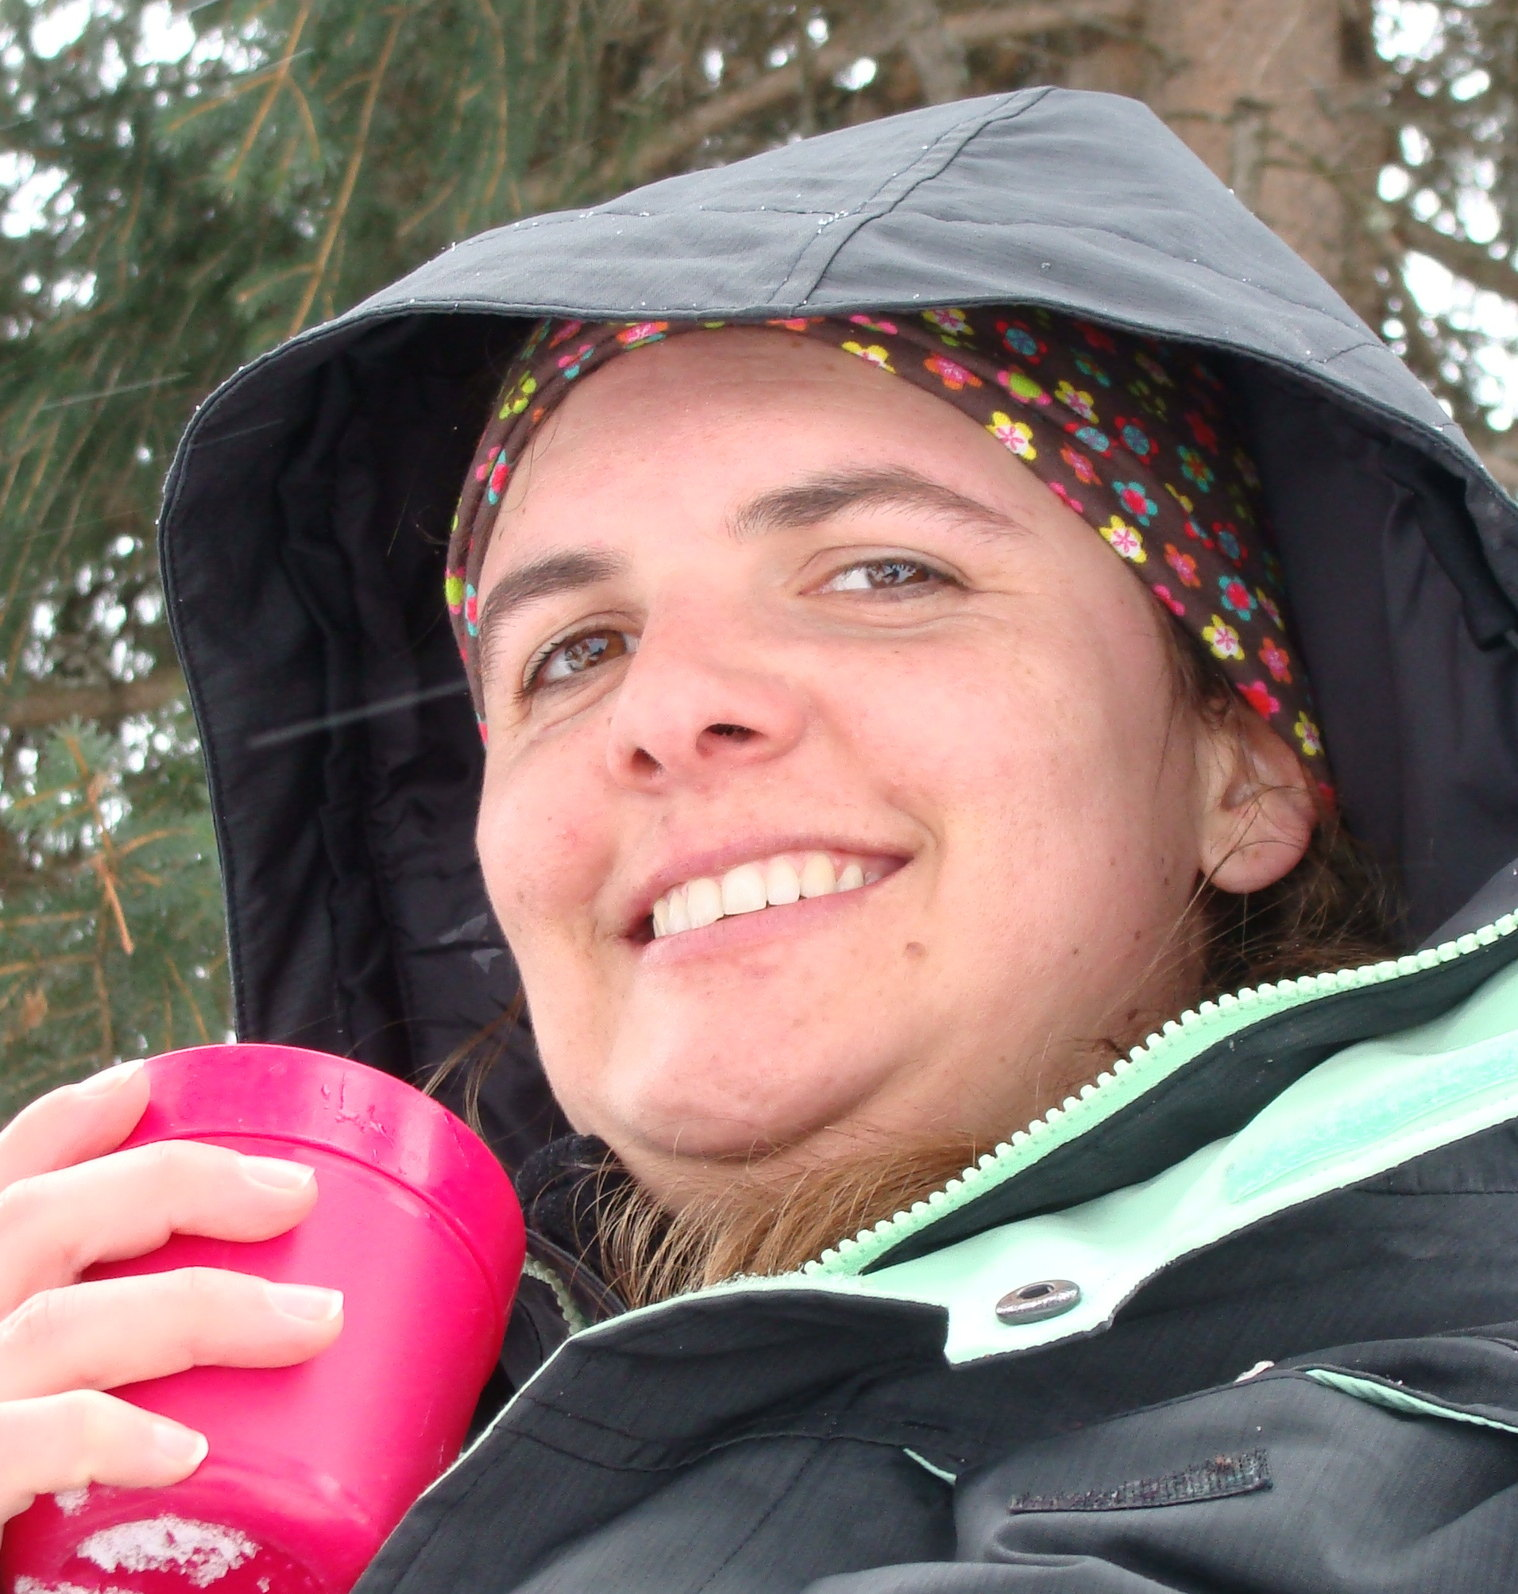
\includegraphics[width = 0.18 \textwidth]{Figures/Judith}};
				
				\node (nina) at ($(koen)+(0,-1.4)$) {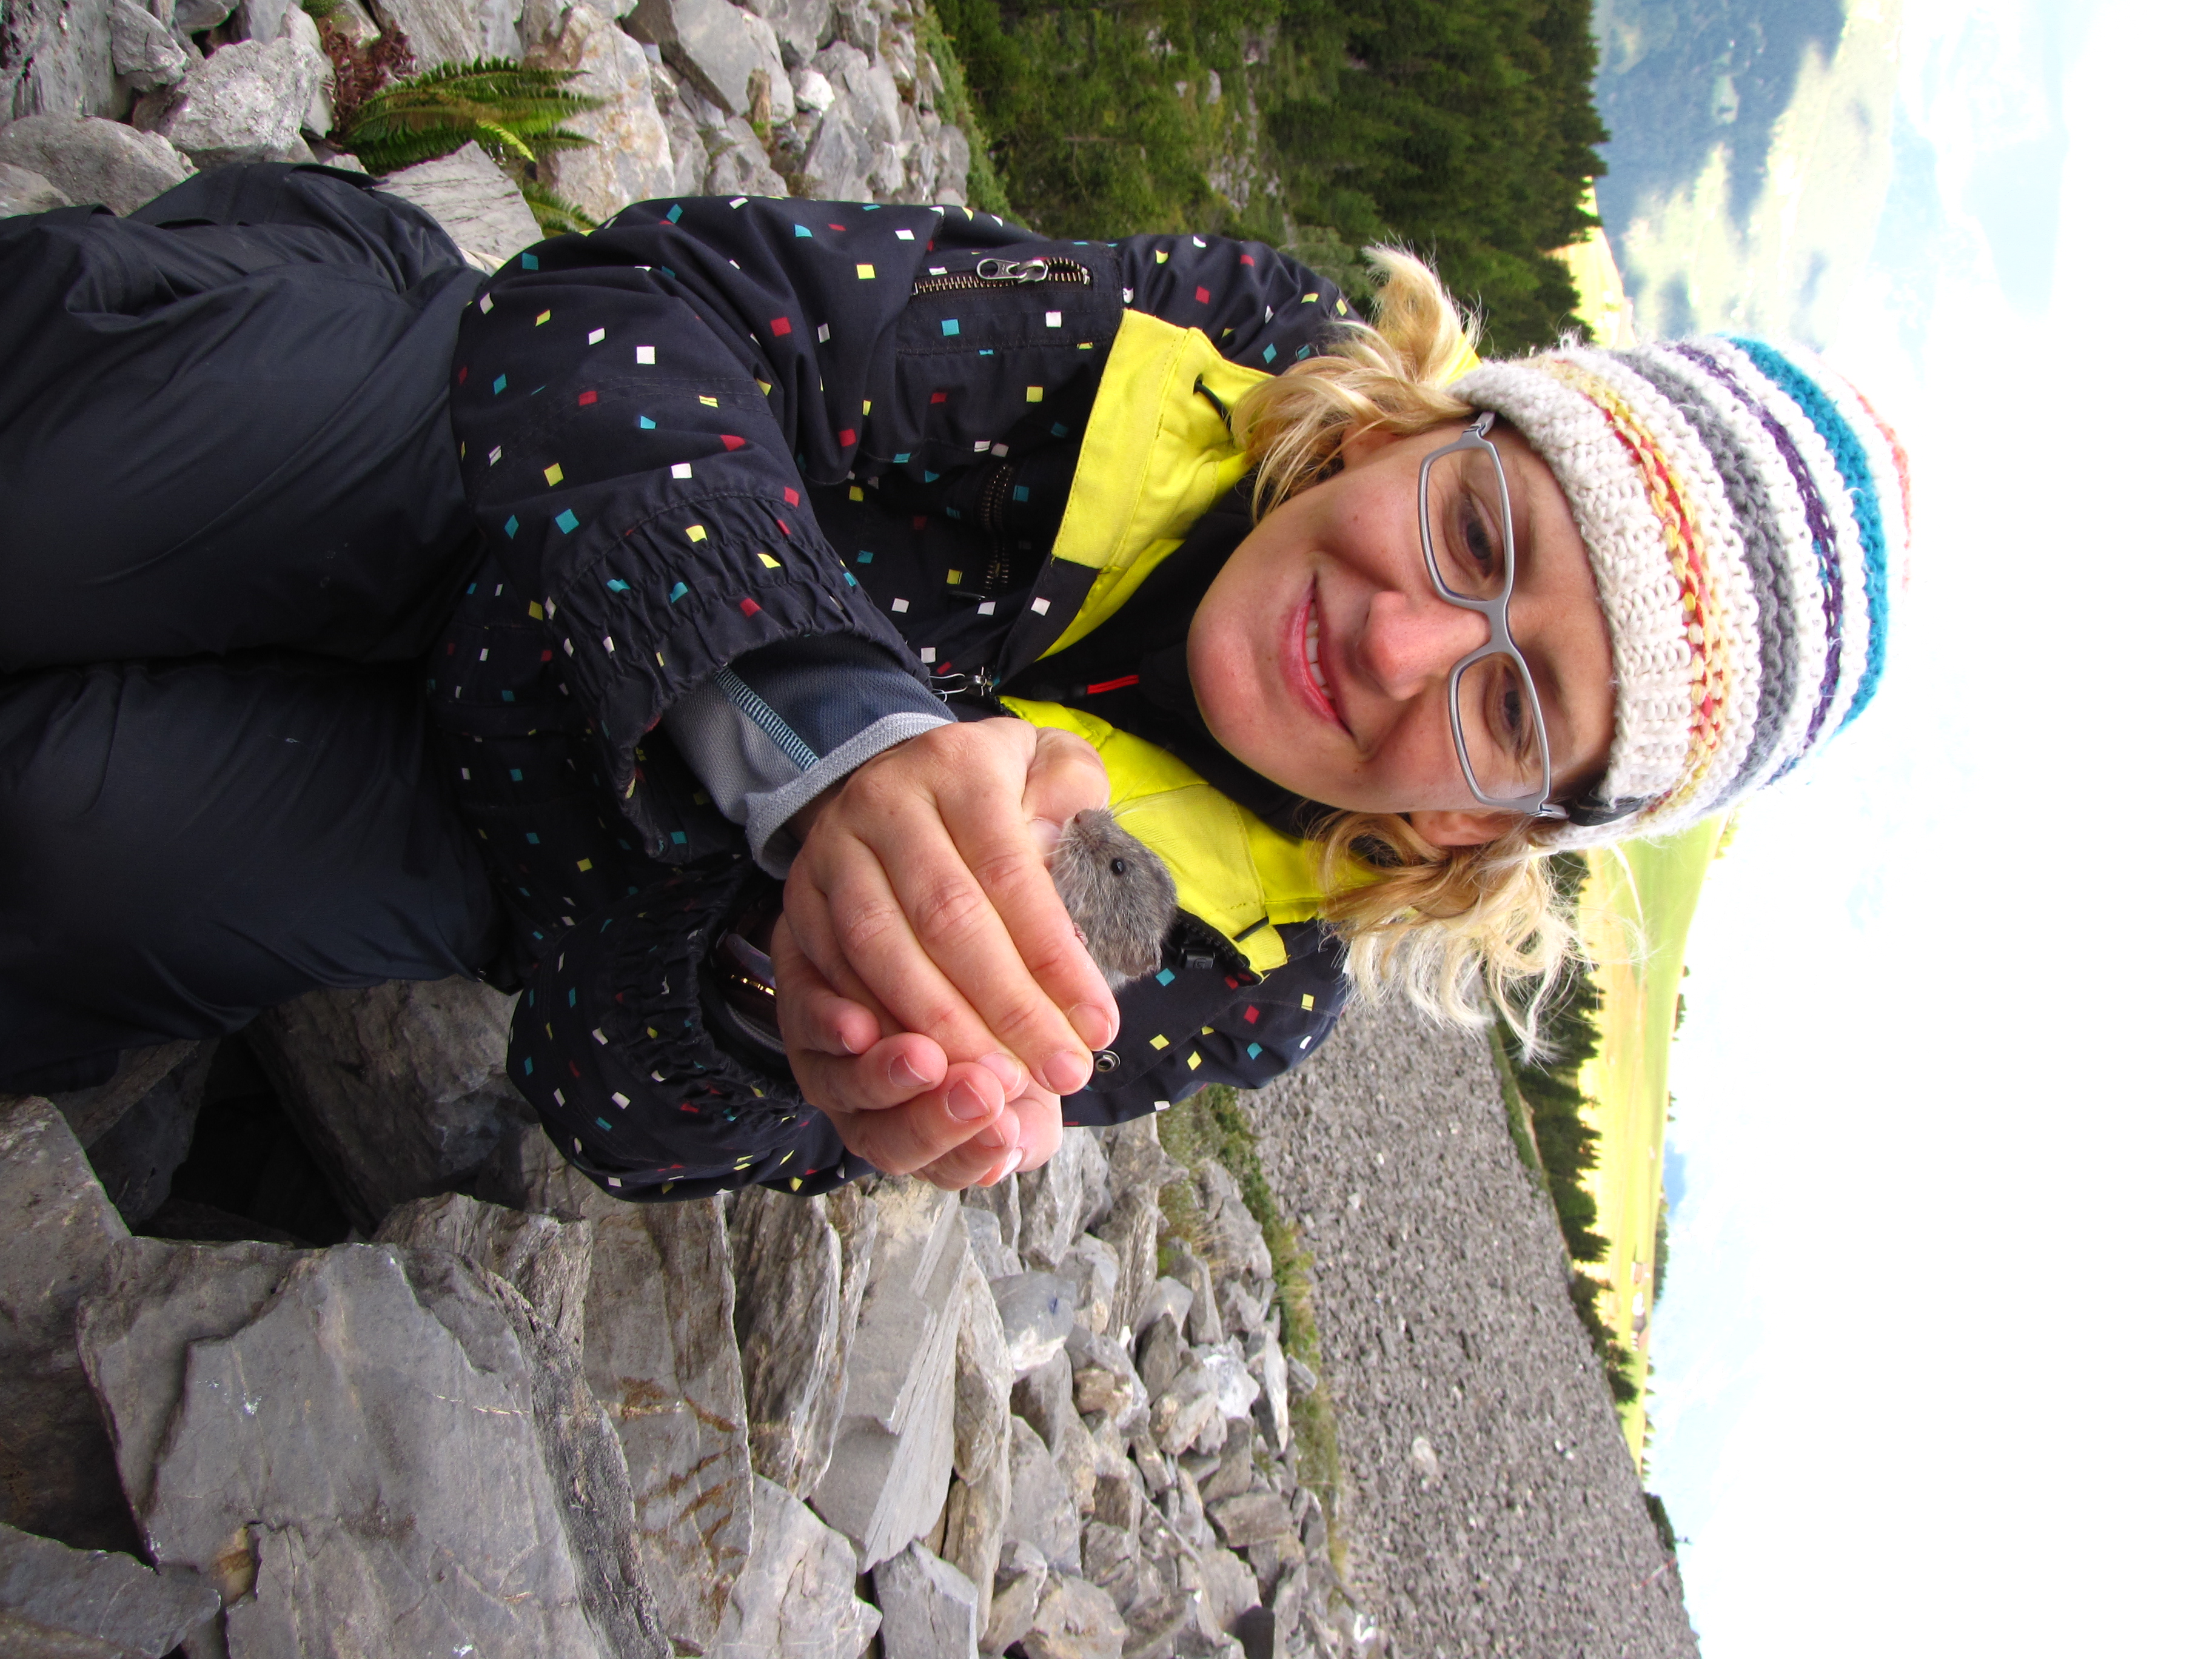
\includegraphics[width = 0.2 \textwidth]{Figures/Nina}};
				\node (hedwig) at ($(nina)+(1.2,0)$) {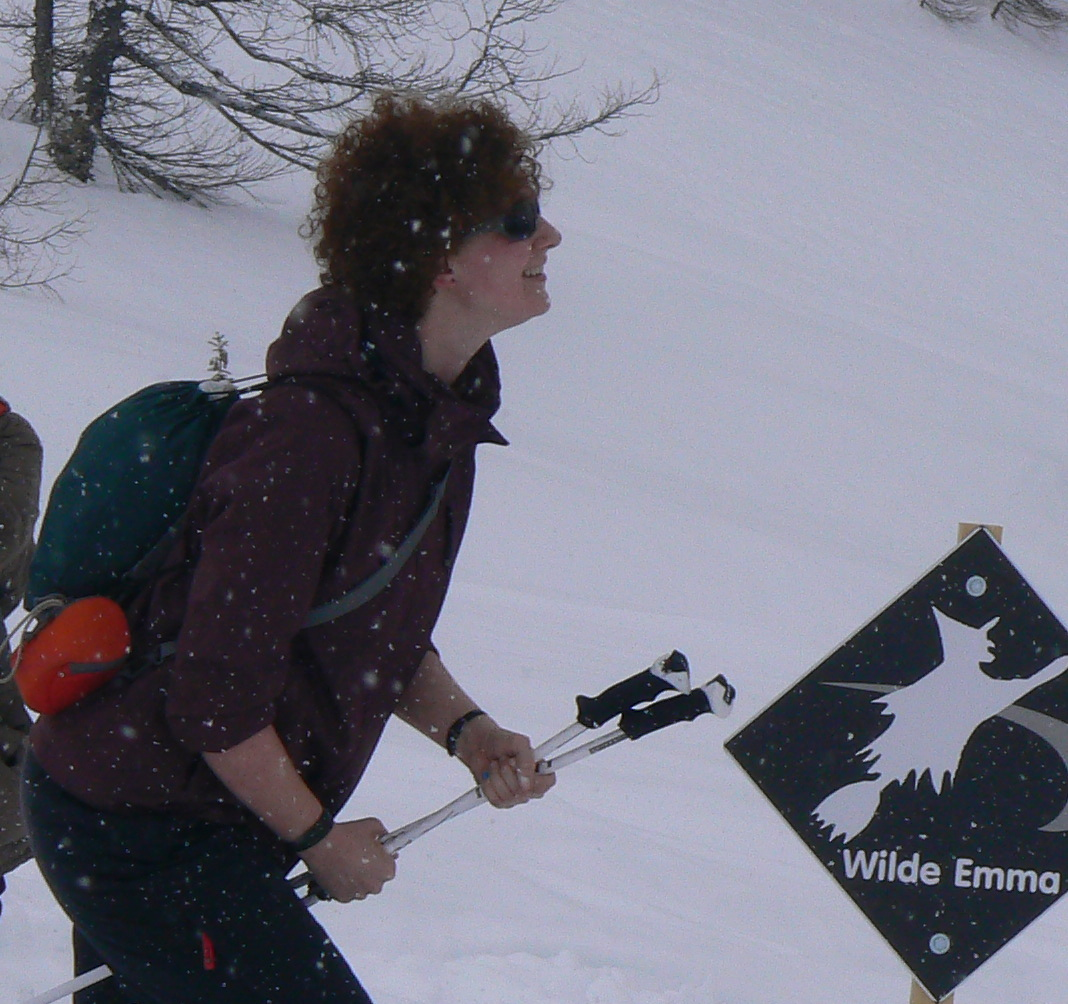
\includegraphics[width = 0.2 \textwidth]{Figures/Hedwig}};
				\node (kasia) at ($(hedwig)+(1.2,0)$) {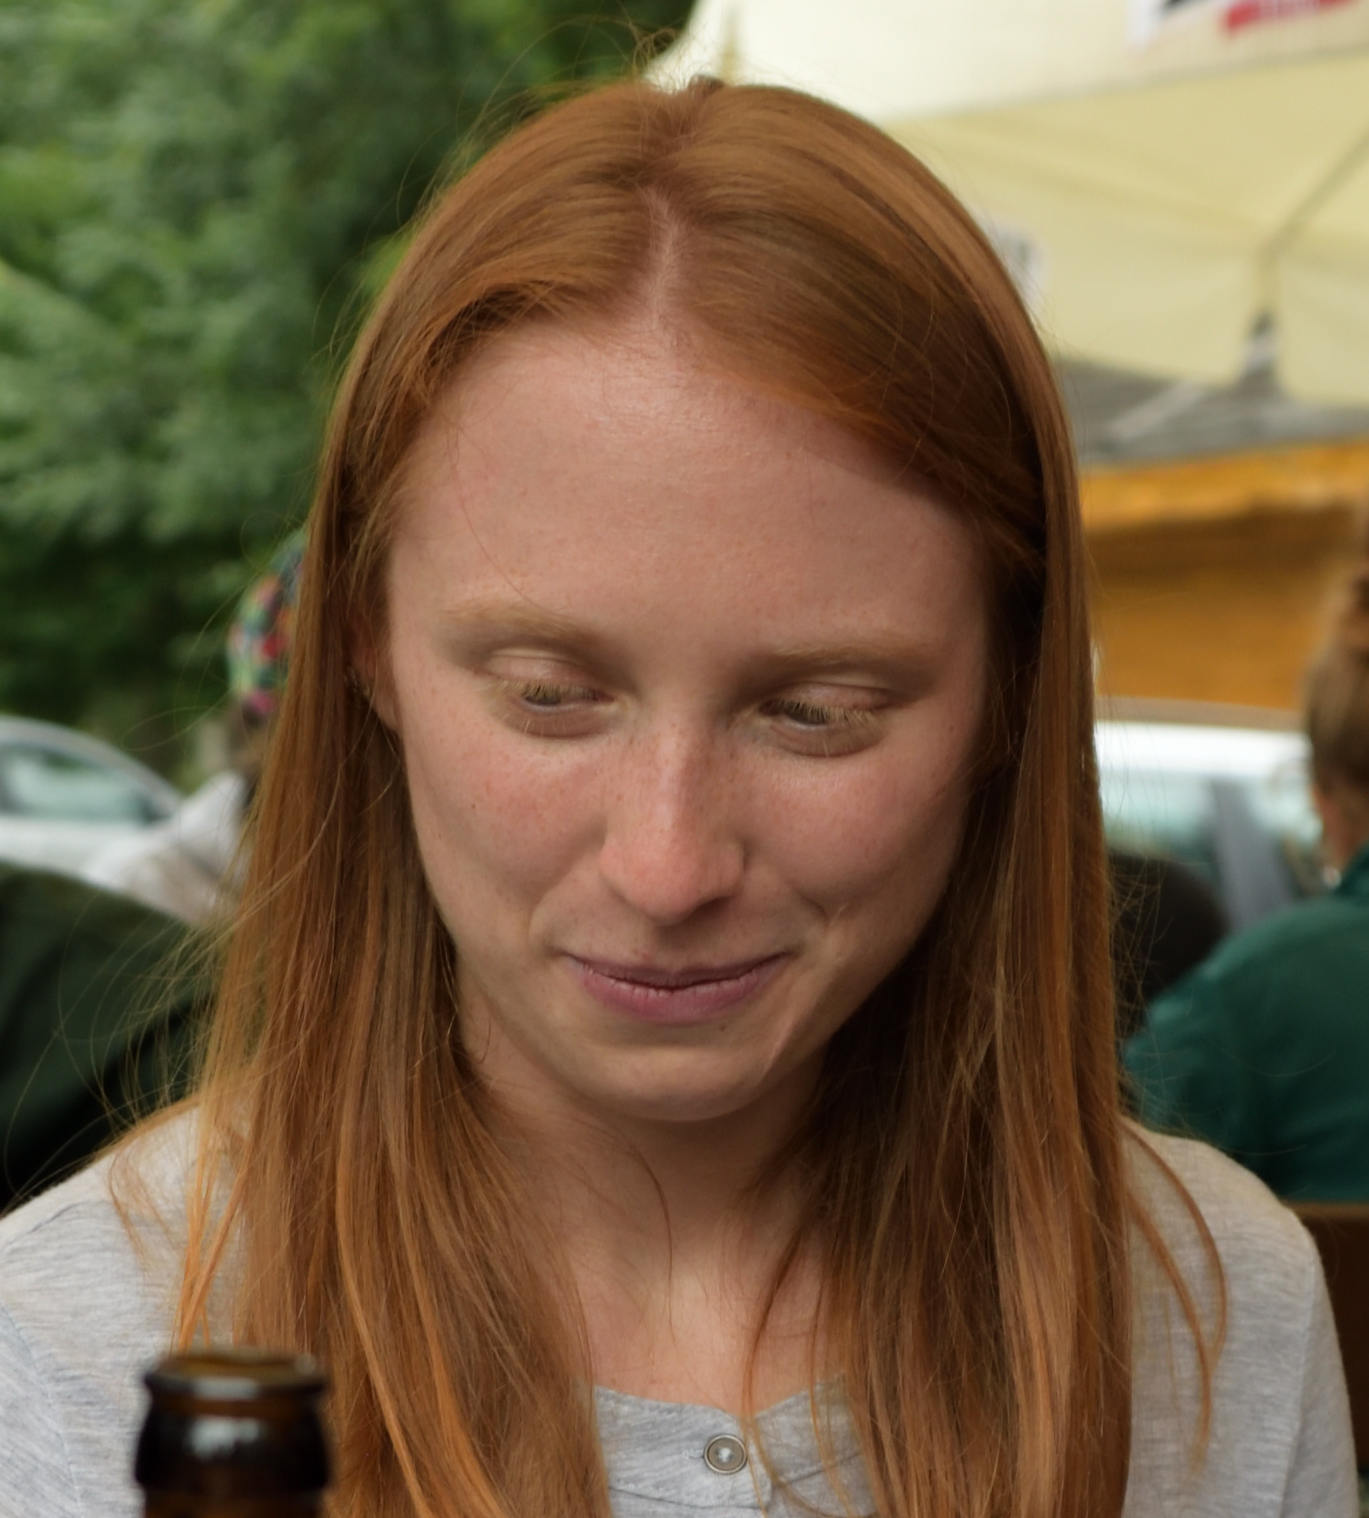
\includegraphics[width = 0.2 \textwidth]{Figures/Kasia}};
				\node (simon) at ($(kasia)+(1.2,0)$) {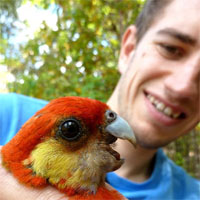
\includegraphics[width = 0.15 \textwidth]{Figures/Simon}};
				\node (chelsea) at ($(simon)+(1.3,0)$) {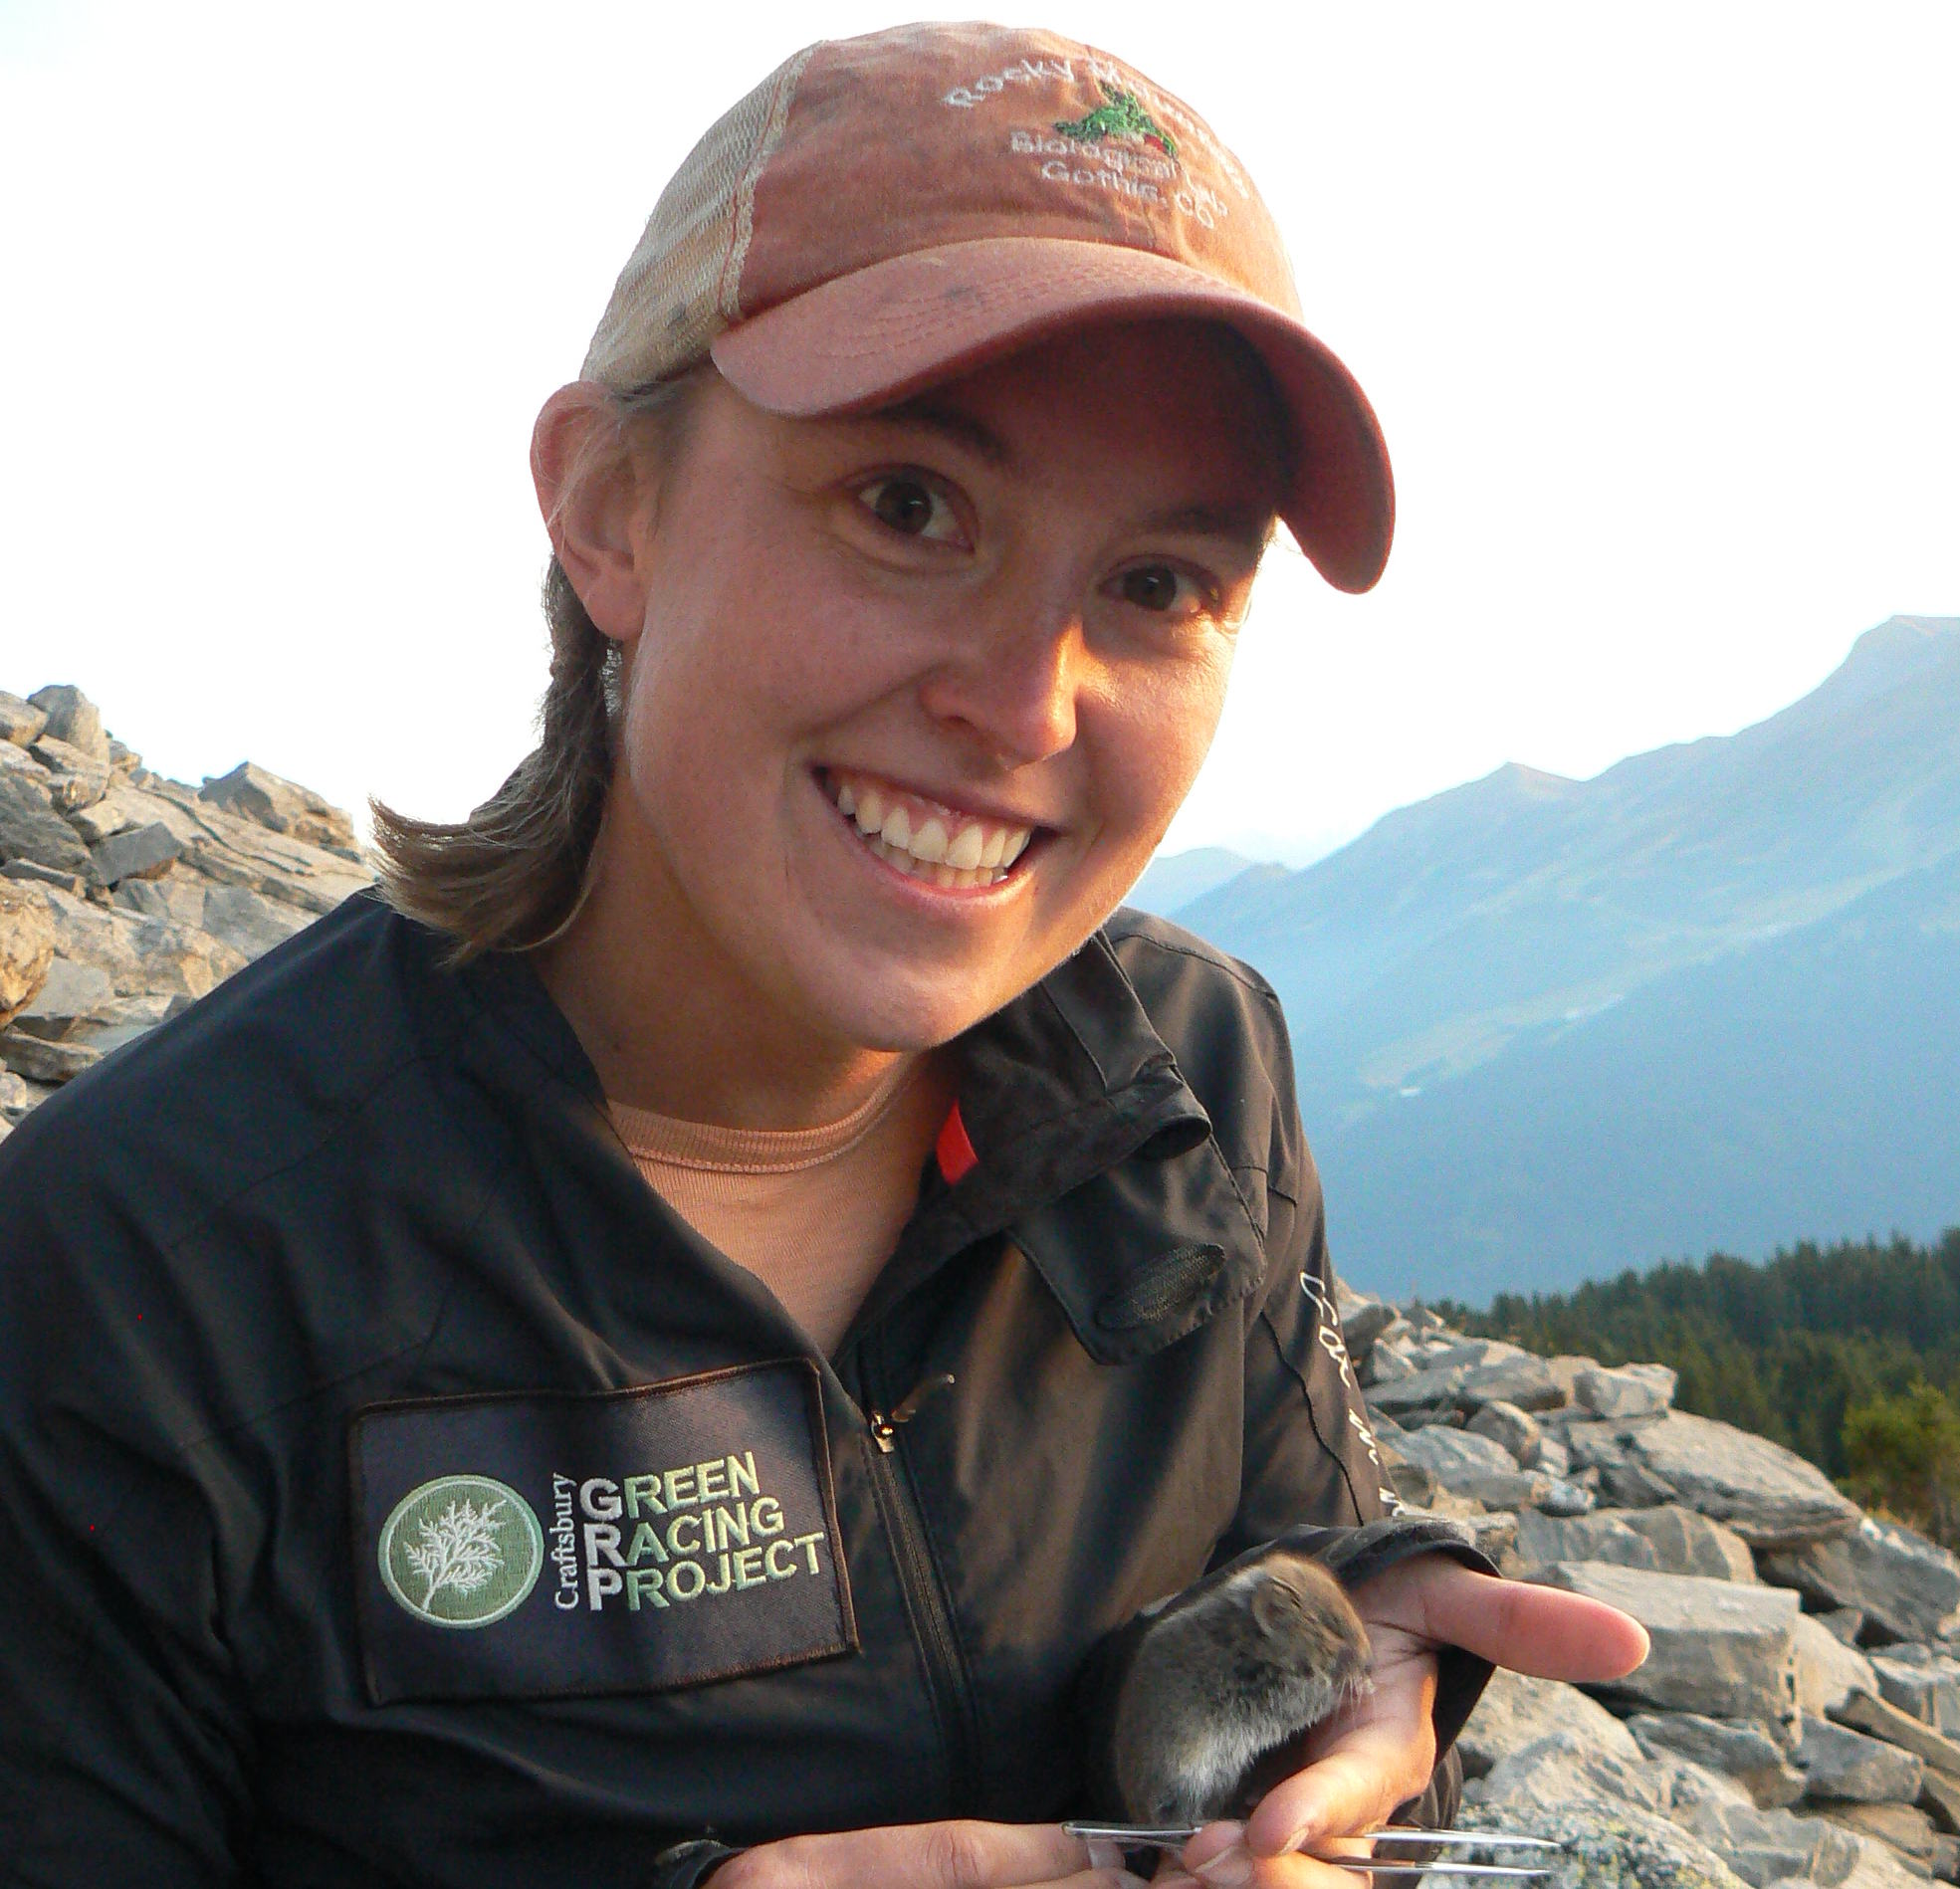
\includegraphics[width = 0.2 \textwidth]{Figures/Chelsea}};
				\node (ashley) at ($(chelsea)+(1.2,0)$) {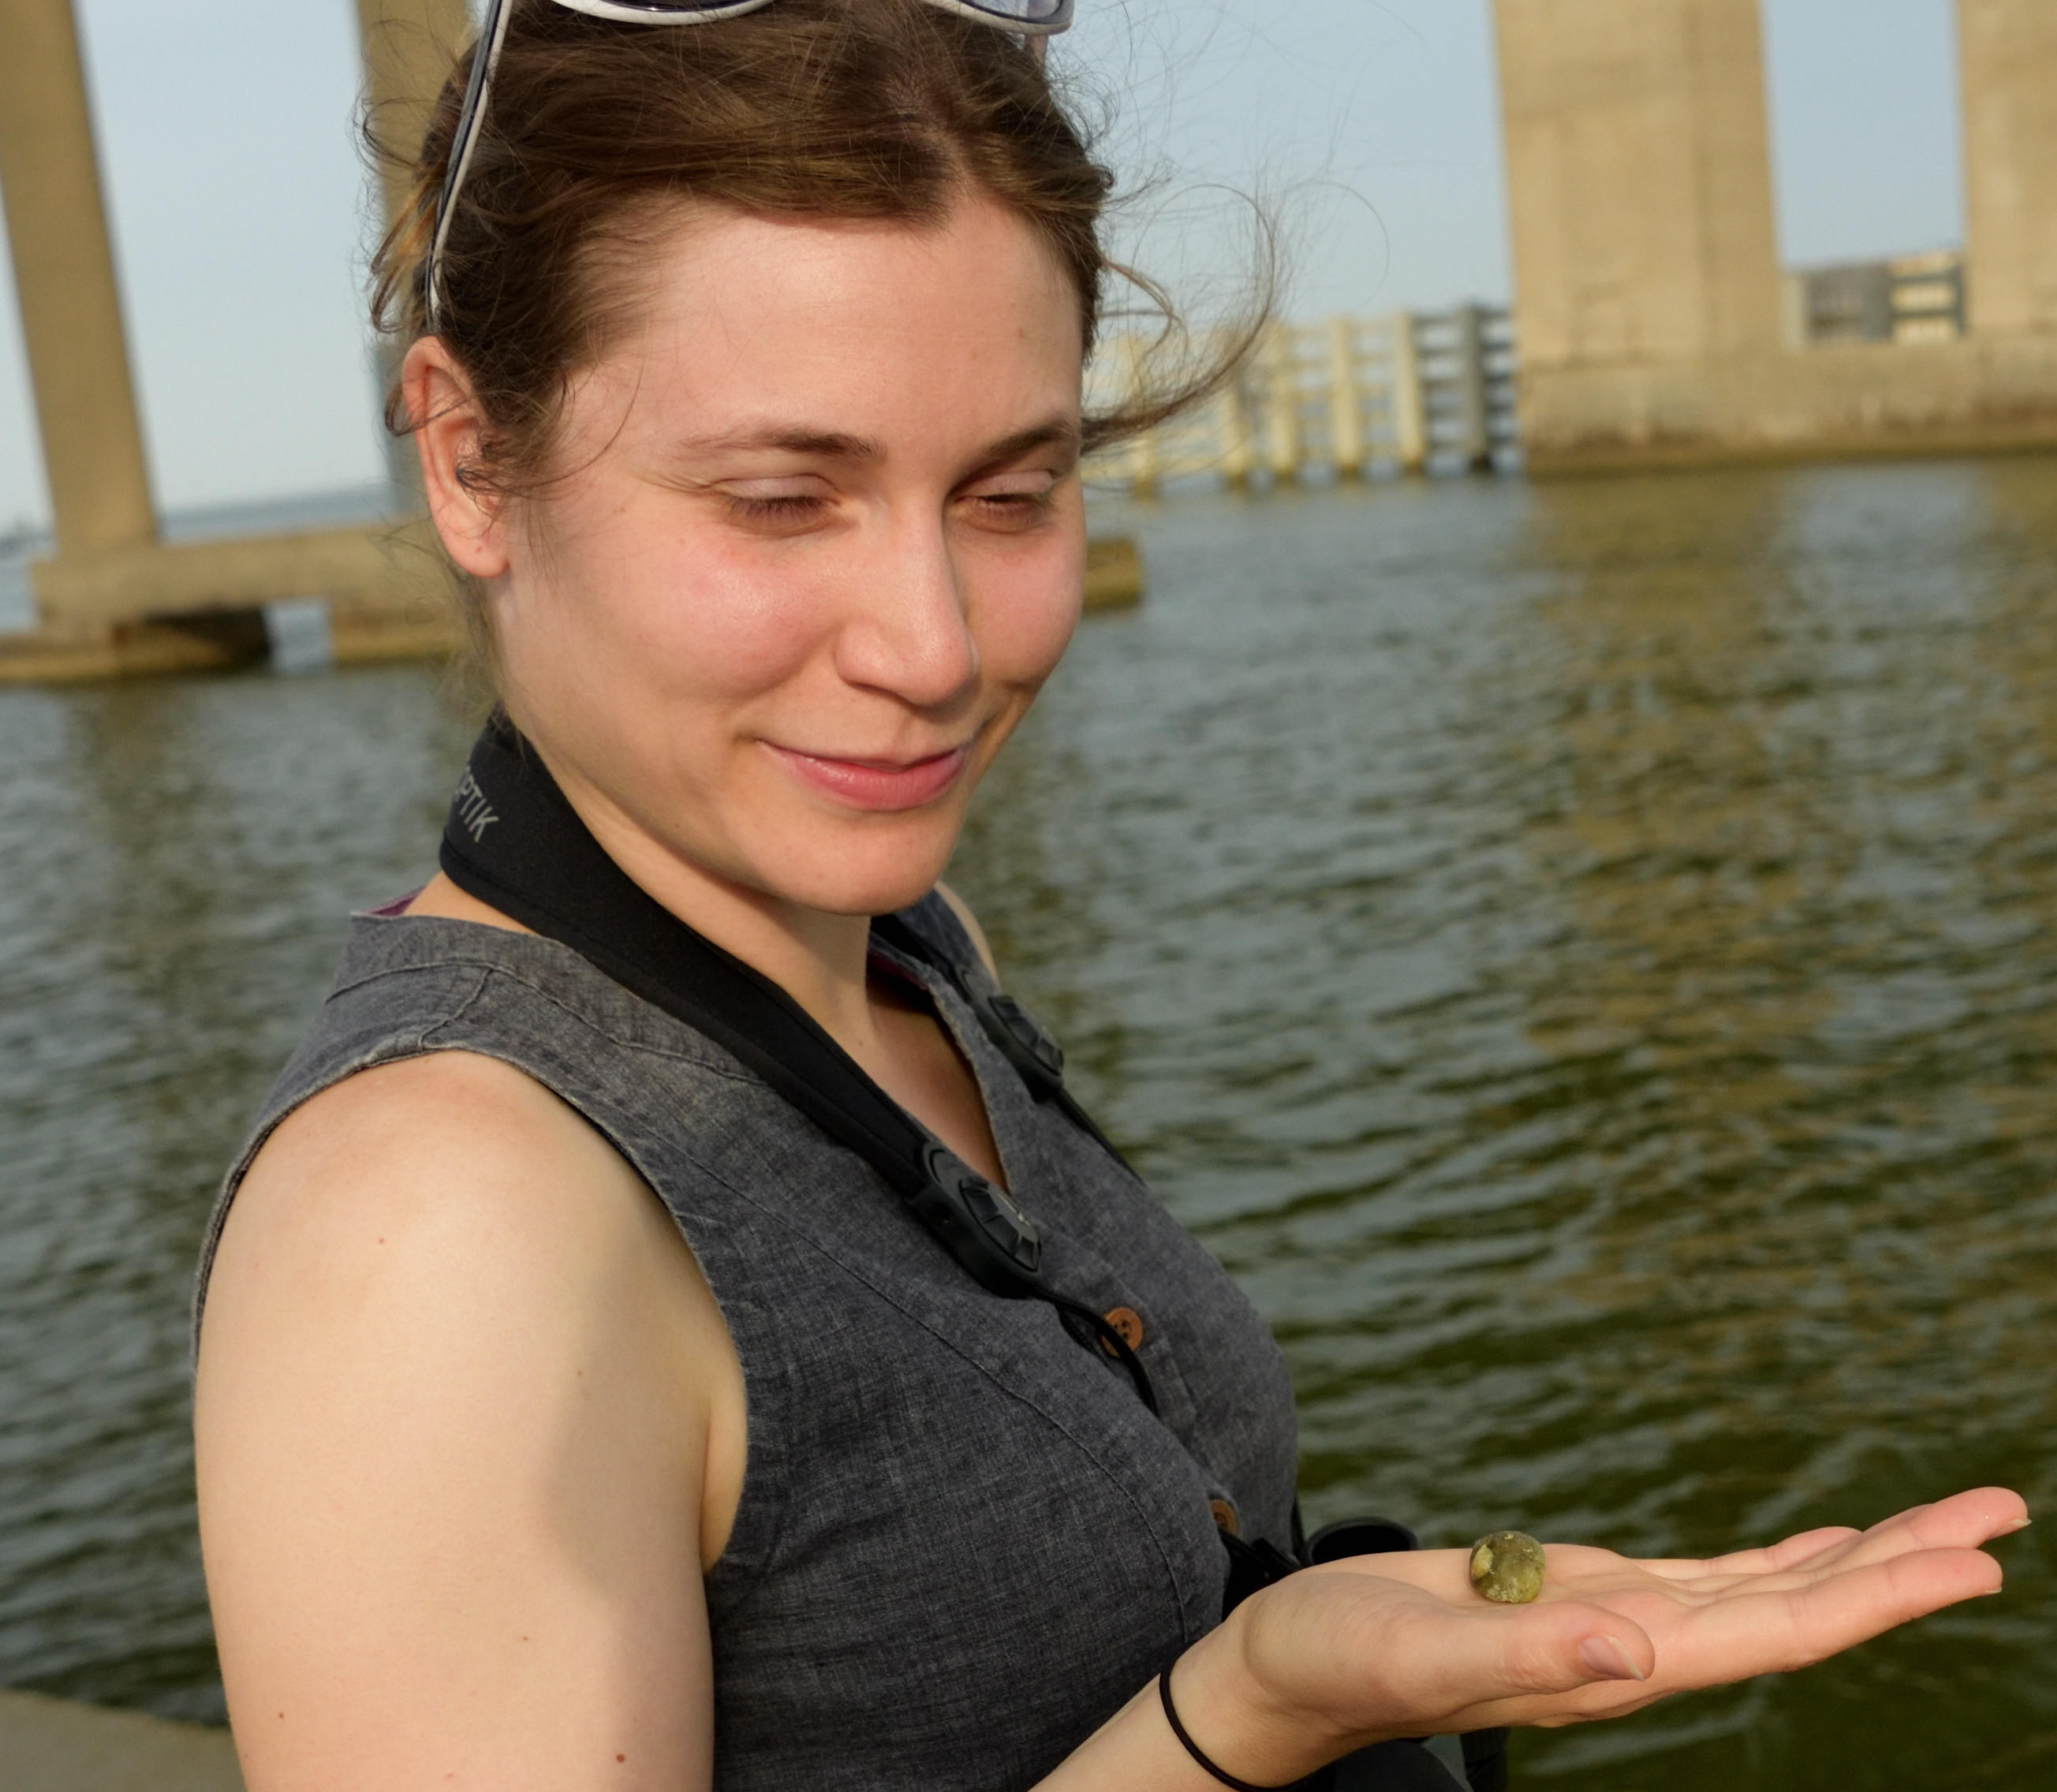
\includegraphics[width = 0.2 \textwidth]{Figures/Ashley}};

%%%%%%		
				\node (beni) at ($(nina)+(0,-1.4)$) {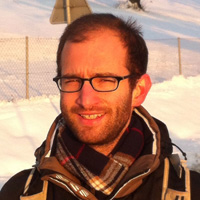
\includegraphics[width = 0.2 \textwidth]{Figures/Beni}};
				\node (alex) at ($(beni)+(1.2,0)$) {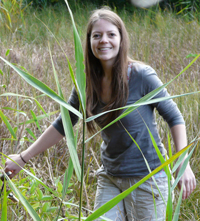
\includegraphics[width = 0.2 \textwidth]{Figures/Alex}};
				\node (rassim) at ($(alex)+(1.2,0)$) {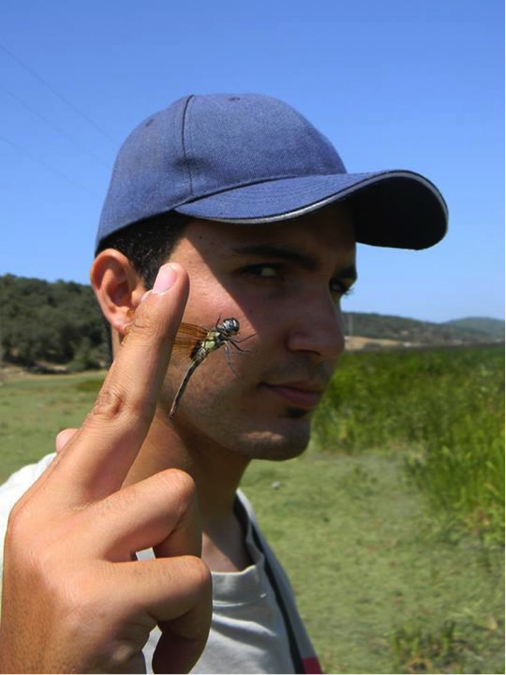
\includegraphics[width = 0.2 \textwidth]{Figures/Rassim}};
				\node (debbie) at ($(rassim)+(1.2,0)$) {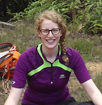
\includegraphics[width = 0.2 \textwidth]{Figures/Debbie}};
				\node (gianalberto) at ($(debbie)+(1.2,0)$) {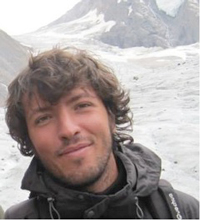
\includegraphics[width = 0.2 \textwidth]{Figures/Gianalberto}};
				\node (peter) at ($(gianalberto) +(1.2,0)$) {\includegraphics[width = 0.2 \textwidth]{Figures/Peter}};
				%%%%
				\node (jelena) at ($(beni)+(0,-1.4)$) {\includegraphics[width = 0.2 \textwidth]{Figures/Jelena}};
				\node (hanna) at ($(jelena)+(1.2,0)$) {\includegraphics[width = 0.2 \textwidth]{Figures/Hanna}};
				\node (jasmin) at ($(hanna)+(1.2,0)$) {\includegraphics[width = 0.2 \textwidth]{Figures/Jasmin}};
				\node (josh) at ($(jasmin)+(1.2,0)$)  {\includegraphics[width = 0.2 \textwidth]{Figures/Josh}};
				\node (wolf) at ($(josh)+(1.2,0)$) {\includegraphics[width = 0.2 \textwidth]{Figures/Wolf}};
				\node (bea) at ($(koen)+(0,-1.4)$) {\includegraphics[width = 0.2 \textwidth]{Figures/Bea}};
				\node (ninag) at ($(koen)+(0,-1.4)$) {\includegraphics[width = 0.2 \textwidth]{Figures/NinaG}};
				\node (anais) at ($(koen)+(0,-1.4)$) {\includegraphics[width = 0.2 \textwidth]{Figures/Anais}};
				\node (isobel) at ($(koen)+(0,-1.4)$) {\includegraphics[width = 0.2 \textwidth]{Figures/Isobel}};
				\node (erika) at ($(koen)+(0,-1.4)$) {\includegraphics[width = 0.2 \textwidth]{Figures/Erika}};
				\node (rien) at ($(koen)+(0,-1.4)$) {\includegraphics[width = 0.2 \textwidth]{Figures/Rien}};
				\node (vanja) at ($(koen)+(0,-1.4)$) {\includegraphics[width = 0.2 \textwidth]{Figures/Vanja}};
				
				\node (christine) at ($(koen)+(0,-1.4)$) {\includegraphics[width = 0.2 \textwidth]{Figures/Christine}};
				
				
			\end{tikzpicture}
		\end{figure}
	\end{column}
	\end{columns}
\end{frame}
%%%%%%%%%%%
%Intro on variation within species/population
%Explain causes of variation imply consequences

\begin{frame}{Phenotypic variation within population}
	\begin{figure}
		\includegraphics[width = 0.6 \textwidth]{Figures/Humansize}
	\end{figure}
	\begin{figure}
		\includegraphics[width = 0.45 \textwidth]{Figures/Cepaea}\hspace{0.1cm}		
		\includegraphics[width = 0.45 \textwidth]{Figures/Harmonia}
	\end{figure}
\end{frame}
%%%%%%%%%%%

\begin{frame}{Phenotypic variation within population}
	\begin{figure}
		\includegraphics[width=0.4\textwidth,height=0.3\textwidth]{Figures/babyTurtle} \hspace{1pt}
		\includegraphics[width=0.4\textwidth,height=0.3\textwidth]{Figures/adultTurtle}
		\vspace{1pt}
		\includegraphics[width=0.4\textwidth,height=0.3\textwidth]{Figures/BlueTits2}\hspace{1pt}
		\includegraphics[width=0.4\textwidth,height=0.3\textwidth]{Figures/BlueTits8}
	\end{figure}
\end{frame}
%%%%%%%%%%%

\begin{frame}{Fitness variation}
	\begin{figure}
		\includegraphics[width=0.2\textwidth,height=0.15\textwidth]{Figures/babyTurtle} \hspace{1pt}
		\includegraphics[width=0.2\textwidth,height=0.15\textwidth]{Figures/adultTurtle}
		\vspace{1pt}
		\includegraphics[width=0.2\textwidth,height=0.15\textwidth]{Figures/BlueTits2}\hspace{1pt}
		\includegraphics[width=0.2\textwidth,height=0.15\textwidth]{Figures/BlueTits8}
	\end{figure}
	
	\begin{alertblock}{What is fitness?}
		The expected relative contribution of an individual to the next generation
	\end{alertblock}
\end{frame}
%%%%%%%%%%%
%%%%%%%%%%%%%%%%%%%%%%%%%%%%%%%%%%%%%%%%%%%%%%%%%%%%%%
%%%%%%%%%%%%%%%%%%%%%%% Chap 1 %%%%%%%%%%%%%%%%%%%%%%%
%%%%%%%%%%%%%%%%%%%%%%%%%%%%%%%%%%%%%%%%%%%%%%%%%%%%%%
\section{Chance or fate? Why do survival and fertility vary?}
%Dice!
%random graph
%reality graph + examples
%two hypotheses for reality
%one dominant for a long time, challenged by new method
%
\begin{frame}

		\only<1>{
			\begin{figure}
				\includegraphics[width=\textwidth]{Figures/figure/dice1-1.pdf}
			\end{figure}}
		\only<2>{
			\begin{figure}
				\includegraphics[width=\textwidth]{Figures/figure/dice1-2.pdf}
			\end{figure}}
		\only<3>{
			\begin{figure}
				\includegraphics[width=\textwidth]{Figures/figure/dice1-3.pdf}
			\end{figure}}
		\only<4>{
			\begin{figure}
				\includegraphics[width=\textwidth]{Figures/figure/dice1-4.pdf}
			\end{figure}}
		\only<5>{
			\begin{figure}
				\includegraphics[width=\textwidth]{Figures/figure/dice1-5.pdf}
			\end{figure}}
		\only<6>{
			\begin{figure}
				\includegraphics[width=\textwidth]{Figures/figure/dice1-6.pdf}
			\end{figure}}
		\only<7>{
			\begin{figure}
				\includegraphics[width=\textwidth]{Figures/figure/dice1-7.pdf}
			\end{figure}}
	

\end{frame}
%%%%%%%%%%%

\begin{frame}

\begin{columns}
\begin{column}[c]{0.5\textwidth}
	\centering
	\textbf{One dice theory }
		\includegraphics[width=\textwidth]{Figures/figure/dice1-7.pdf}
	\end{column}
\begin{column}[c]{0.5\textwidth}
	\centering
	\uncover<2->{
	\textbf{Real pattern}
		\includegraphics[width=\textwidth]{Figures/figure/dice2-4.pdf}
	}
	
\end{column}
\end{columns}

\begin{columns}
\begin{column}[c]{0.5\textwidth}

\end{column}
\begin{column}[c]{0.5\textwidth}
\centering
	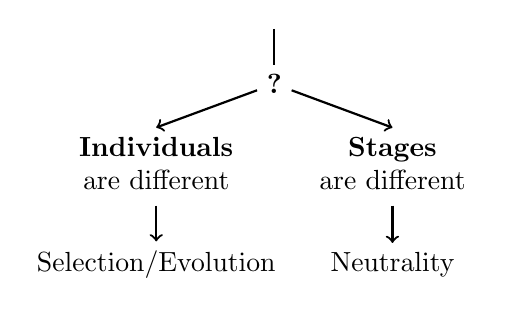
\begin{tikzpicture}
		\uncover<3->{
				\node (q) at (0,-0.7) {\textbf{?}};
				\draw[thick] (0,0) -- (q);
				\node (sel) at (-1.5,-1.5) {\parbox[t][0.2cm][t]{2cm}{\centering \textbf{Individuals} are different}};
				\draw[->, thick] (q) -- (sel.north);
		}
		\uncover<4->{	\node (neutral) at (1.5,-1.5) {\parbox[t][0.2cm][t]{1.9cm}{\centering \textbf{Stages}\\ are different}};
		\draw[->, thick] (q) -- (neutral.north);
		}
		\uncover<5->{
			\node (sh) at (-1.5, -3) {Selection/Evolution};
			\node (ne) at (1.5, -3)  {Neutrality};
			\draw[->, thick] ($(sel.south)+(0,-0.5)$) -- (sh.north);
			\draw[->, thick] ($(neutral.south)+(0,-0.5)$) -- (ne.north);
		}
	
	\end{tikzpicture}
\end{column}
\end{columns}

\end{frame}
%%%%%%%%%%%

\begin{frame}{The neutral theory}
\includegraphics[width=\textwidth]{Figures/NeutralTheory}

\textbf{Neutral matrix method}
\vspace{0.5cm}
\begin{columns}
\begin{column}[c]{0.5\textwidth}
\begin{table}
\begin{tabular}{c|c c c}
& \multicolumn{3}{c}{next year} \\
	& 1 & 2 & 3\\
	\hline
1	& \color{red!90}{0.9}	&	 \color{red!8}{0.08}	&	 \color{red!2}{0.02}	\\
2 & 0  	&	\color{red!70}{0.7}	&	 \color{red!30}{0.3}	\\
3 & 0  	&	 \color{red!20}{0.2}	&	\color{red!80}{0.8}	\\

\end{tabular}
\end{table}
\end{column}
\begin{column}[c]{0.5\textwidth}
	\only<3>{
	\vspace{-1cm}
		\begin{figure}
		\includegraphics[width=1\textwidth]{Figures/figure/lrssimul-1.pdf}
		\end{figure}}
	\only<4>{
	\vspace{-1cm}
	\begin{figure}
	\includegraphics[width=1\textwidth]{Figures/figure/lrssimul-3.pdf}
	\end{figure}}
\end{column}
\end{columns}
\centering
\textbf{\color{OwlRed}{No variation in fitness among individuals}}
\end{frame}
%%%%%%%%%%%
\begin{frame}{Conflicting results}
\begin{columns}
	\begin{column}[c]{0.5\textwidth}
	\textbf{\color{OwlRed}{Neutral matrix method}}
	\begin{itemize}
		\uncover<2->{\item No significant differences between individuals}
		\uncover<4->{\item \dots because of stage structure}
		\uncover<6->{\item \dots very little and due to chance only}
	\end{itemize}
	
	\end{column}
	\begin{column}[c]{0.5\textwidth}
	\textbf{\color{OwlBlue}{Mixed model method \& Quantitative genetics}}

	\begin{itemize}
		\uncover<3->{\item Individual performances are repeatable}
		\uncover<5->{\item \dots fitness traits are heritable} 
		\uncover<7->{\item \dots eh?}
	\end{itemize}
	
	\end{column}
\end{columns}

\begin{figure}
	\only<1>{\includegraphics[width=0.4\textwidth]{Figures/Kittiwake}}
	\only<2>{\includegraphics[width=0.8\textwidth]{Figures/Steinerkittiwake}}
	\only<3>{\vspace{-2cm} \includegraphics[width=0.8\textwidth]{Figures/CamKittiwake}}
	\only<4>{\vspace{-1.5cm}\includegraphics[width=0.8\textwidth]{Figures/figure/dice2-4.pdf}\vspace{-1.5cm}}
\end{figure}

\only<8>{\begin{block}{Why?}
	\begin{itemize}
		\item \textbf{\color{OwlRed}{Neutral matrix method}} =\textbf{false negative}?
		\item \textbf{\color{OwlBlue}{Mixed model method}} =\textbf{false positive}?
	\end{itemize}
\end{block}}

\end{frame}
%%%%%%%%%%%

\begin{frame}{Method}
\begin{figure}
\begin{tikzpicture}[%
  % common options for blocks:
  block/.style = {draw, align=center, anchor=north,
              minimum height=0.50cm, inner sep=1pt,fill=black!80},
	roundblock/.style = {draw, align=center, anchor=north,
              minimum height=2cm, inner sep=2pt,rounded corners=3pt,fill=black!80},
	backblock/.style = {fill=gray!90, align=center, anchor=west,
               inner sep=2pt,rounded corners=3pt},
  % common options for the circles:
  ball/.style = {circle, draw, align=center, anchor=north, inner sep=0},
	oval/.style = {ellipse, draw, align=center, anchor=north, inner sep=1pt,fill=white}
	]
\footnotesize	
\node[backblock,minimum width=5.25cm,minimum height=5.2cm] (Abb) at (-4,-1) {};
\node[backblock,fill=gray!75,minimum width=5.25cm,minimum height=5.2cm] (Bbb) at ($(Abb.east) +(0.25,0)$) {};
\node[] (a) at ($(Abb.north)+(-1,-0.25)$){\textbf{Simulate data}};
\node[] (b) at ($(Bbb.north)+(-0.5,-0.25)$) {\textbf{Test fixed heterogeneity}};

\node[roundblock,text width=2cm, anchor=west] (Parameters) at ($(Abb.west)+(0.25,0)$) {\textbf{Parameters}\\ Fertility, Viability, Persistence, \textbf{\color{OwlYellow}{Individual differences}}};

{\scriptsize 
\node[block,text width=1.5cm] (scenario1) at ($(Parameters.north)+(2.2,0)$) {Scenario 1};
\node[text width=2cm, align=center] (par) at ($(scenario1)+(0,0.8)$) {Parameter};
\node[text width=2cm, align=center] (comb) at ($(par)+(0,-0.3)$) {combinations};
\node[block,text width=1.5cm] (scenario2) at ($(scenario1)+(0,-0.6)$) {Scenario 2};
\node[] (scenarion) at ($(scenario1)+(0,-1.45)$) {\textbf{\vdots}};
\node[block,text width=1.5cm] (scenario240) at ($(scenario1)+(0,-2)$) {Scenario 249};
}

\draw[->,shorten >= 2pt] (Parameters.east) to (scenario1.west);
\draw[->,shorten >= 2pt] (Parameters.east) to (scenario2.west);
\draw[->,shorten >= 2pt] (Parameters.east) to (scenario240.west);


{\scriptsize 
\coordinate (stos) at (1.8,0);
\node[backblock,text width=1.8cm, anchor=west, fill=black!80] (simdata1) at ($(scenario1.west) + (stos)$) {1000 data sets};
\node[backblock,text width=1.8cm, anchor=west, fill=black!80] (simdata2) at ($(scenario2.west) + (stos)$) {1000 data sets};
\node[] (simn) at ($(scenarion)+(stos)$) {\textbf{\vdots}};
\node[backblock,text width=1.8cm, anchor=west, fill=black!80] (simdata240) at ($(scenario240.west) + (stos)$) {1000 data sets};
}

\draw[->] (scenario1.east) to (simdata1.west);
\draw[->] (scenario2.east) to (simdata2.west);
\draw[->] (scenario240.east) to (simdata240.west);

{\scriptsize 
\gettikzxy{(simdata1.east)}{\ax}{\ay}
\gettikzxy{(Parameters.north)}{\px}{\py}
\coordinate (cordtest) at ($(\ax,\py)+(2.5,0)$);
\node[roundblock,text width=3cm,minimum height=0.2cm] (test) at (cordtest) {\tikz{\node[anchor=north] (ts) at (0.125,0.6) {\centering\textbf{\color{OwlYellow}{Individual differences?}}};
\node[roundblock,text width=2.6cm,minimum height=0.2cm] (MM) at (0,-0.1) {\parbox[t][0.2cm][t]{2.6cm}{\centering\textbf{\color{OwlBlue}{Mixed models}}}};
\node[roundblock,text width=2.6cm,minimum height=0.2cm] (MM) at (0,-0.6) {\parbox[t][0.2cm][t]{2.6cm}{\centering\textbf{\color{OwlRed}{Neutral matrices}}}};
}};
}

\draw[->,shorten >= 2pt] (simdata1.east) to (test.170);
\draw[->,shorten >= 2pt] (simdata2.east) to (test.180);
\draw[->,shorten >= 2pt] (simdata240.east) to (test.190);

\node[block, anchor=south] (error) at ($(Bbb.south)+(0,0.25)$) {False positive and false negative rates};

\draw[->, shorten >= 2pt] (test.270) to (error.90);

\end{tikzpicture}
\end{figure}
\end{frame}
%%%%%%%%%%%

\begin{frame}{Results}
\only<1>{
\begin{figure}
	\includegraphics[width=\textwidth]{Figures/figure/resultsdynhet-2.pdf}
\end{figure}}
\only<2>{
\begin{figure}
	\includegraphics[width=\textwidth]{Figures/figure/resultsdynhet-3.pdf}
\end{figure}}
\only<3>{
\begin{figure}
	\includegraphics[width=\textwidth]{Figures/figure/resultsdynhet-4.pdf}
\end{figure}}
	
\end{frame}
%%%%%%%%%%%
\begin{frame}{Conclusion}

\begin{block}{Why conflicting methods?}
	\uncover<2->{\begin{itemize}
		\item \textbf{\color{OwlRed}{Neutral matrix method}} =\textbf{false negative}? \textbf{\color{red}{YES}}
		\item \textbf{\color{OwlBlue}{Mixed model method}} =\textbf{false positive}? \textbf{\color{red}{NO}}
	\end{itemize}}
	\uncover<3->{$\rightarrow$ Individual differences in fitness components are common}
\end{block}

	\uncover<4->{\begin{block}{Implications}
		\begin{itemize}
			\uncover<5->{\item Phenotypic variation in fitness $\rightarrow$ opportunity for selection}
			\uncover<6->{\item Heritability of fitness $=$ \textbf{evolution}}
		\end{itemize}
	\end{block}}
	
	\uncover<6->{
	\begin{figure}
		\begin{tikzpicture}
			\node (f) at (-1,0) {\includegraphics[width = 0.2\textwidth]{Figures/Fisher}};
			\node (fn) at ($(f.south)+(0,-0.2)$) {\textbf{R.A. Fisher}};
			\node (p) at (1,0) {\includegraphics[width = 0.2\textwidth]{Figures/Price}};
			\node (fn) at ($(p.south)+(0,-0.2)$) {\textbf{G. Price}};
		\end{tikzpicture}
	\end{figure}}
\end{frame}
%%%%%%%%%%%
\begin{frame}
\begin{figure}
	\includegraphics[width=\textwidth]{Figures/Dynhet}
\end{figure}
\end{frame}
%%%%%%%%%%%

\begin{frame}
\end{frame}
%%%%%%%%%%%
%%%%%%%%%%%%%%%%%%%%%%%%%%%%%%%%%%%%%%%%%%%%%%%%%%%%%%
%%%%%%%%%%%%%%%%%%%%%%% Chap 2 %%%%%%%%%%%%%%%%%%%%%%%
%%%%%%%%%%%%%%%%%%%%%%%%%%%%%%%%%%%%%%%%%%%%%%%%%%%%%%

\begin{frame}{Evolution in a changing world}

	\only<1>{\begin{figure}
		\includegraphics[width = 0.6\textwidth]{Figures/ipcc}
		
		Intergovernmental panel on climate change 5th Report (2014)
	\end{figure}}
	
	\only<2>{\begin{figure}
		\includegraphics[width = 0.8\textwidth]{Figures/biodiv}
		
		Newbold \& al. (2016). Has land use pushed terrestrial biodiversity beyond the planetary boundary? A global assessment. Science, 353
	\end{figure}}
	
	\only<3>{\begin{figure}
		\includegraphics[width = 0.8\textwidth]{Figures/parmesan}
		\end{figure}}
	
\end{frame}
%%%%%%%%%%%

\begin{frame}

	\begin{figure}
		\begin{tikzpicture}
			\uncover<1-2>{\node [shading = axis,rectangle, bottom color=green!50!gray, top color=gray, minimum height=2.5cm, minimum width=5.5cm] (hab1) at (0,0) {};}
			
			\uncover<3->{\node [shading = axis,rectangle, bottom color=green, top color=green!50!gray, minimum height=2.5cm, minimum width=5.5cm] (hab1) at (0,0) {};}
			
			\uncover<1>{\node (sun) at ($(hab1.150)+(-1,1)$) {\includegraphics[width = 0.10\textwidth]{Figures/sun.png}};}
			\uncover<2->{\node (sun) at ($(hab1.150)+(-1,1)$) {\includegraphics[width = 0.15\textwidth]{Figures/sun.png}};}
			
			\uncover<1-3>{\node (vole1) at (0,0) {\includegraphics[width = 0.05\textwidth]{Figures/snowwwvole2}};
			\node (vole2) at (1,0.1) {\includegraphics[width = 0.06\textwidth]{Figures/snowwwvole2}};
			\node (vole3) at (-0.7,0.3) {\includegraphics[width = 0.03\textwidth]{Figures/snowwwvole2}};
			\node (vole4) at (-1.5,-0.3) {\includegraphics[width = 0.06\textwidth]{Figures/snowwwvole2}};
			\node (vole5) at (1.7,-0.15) {\includegraphics[width = 0.04\textwidth]{Figures/snowwwvole2}};}
			
			\uncover<4>{
			\node [shading = axis,rectangle, bottom color=green, top color=green!50!gray, minimum height=2.5cm, minimum width=5.5cm] (hab2) at ($(hab1)+(0,0)$) {};
			\node (vole1b) at (0,2) {\includegraphics[width = 0.05\textwidth]{Figures/snowwwvole2}};
			\node (vole2b) at (1,2.3) {\includegraphics[width = 0.06\textwidth]{Figures/snowwwvole2}};
			\node (vole3b) at (-0.7,2.3) {\includegraphics[width = 0.03\textwidth]{Figures/snowwwvole2}};
			\node (vole4b) at (-1.5,1.7) {\includegraphics[width = 0.06\textwidth]{Figures/snowwwvole2}};
			\node (vole5b) at (1.7,1.25) {\includegraphics[width = 0.04\textwidth]{Figures/snowwwvole2}};}	
			
			\uncover<5>{\node (vole1c) at (0,0) {\includegraphics[width = 0.08\textwidth]{Figures/Deadsnowwwvole2}};
			\node (vole2c) at (1,0.1) {\includegraphics[width = 0.09\textwidth]{Figures/Deadsnowwwvole2}};
			\node (vole3c) at (-0.7,0.3) {\includegraphics[width = 0.05\textwidth]{Figures/Deadsnowwwvole2}};
			\node (vole4c) at (-1.5,-0.3) {\includegraphics[width = 0.09\textwidth]{Figures/Deadsnowwwvole2}};
			\node (vole5c) at (1.7,-0.15) {\includegraphics[width = 0.06\textwidth]{Figures/Deadsnowwwvole2}};}

			\uncover<6>{\node (vole1q) at (0,0) {\includegraphics[width = 0.05\textwidth]{Figures/snowwwvole2}};
			\node (vole2q) at (1,0.1) {\includegraphics[width = 0.06\textwidth]{Figures/snowwwvole2}};
			\node (vole3q) at (-0.7,0.3) {\includegraphics[width = 0.03\textwidth]{Figures/snowwwvole2}};
			\node (vole4q) at (-1.5,-0.3) {\includegraphics[width = 0.06\textwidth]{Figures/snowwwvole2}};
			\node (vole5q) at (1.7,-0.15) {\includegraphics[width = 0.04\textwidth]{Figures/snowwwvole2}};}
			
			\uncover<7>{\node (vole1s) at (0,0) {\includegraphics[width = 0.06\textwidth]{Figures/snowwwvole2}};
			\node (vole2s) at (1,0.1) {\includegraphics[width = 0.07\textwidth]{Figures/snowwwvole2}};
			\node (vole3s) at (-0.7,0.3) {\includegraphics[width = 0.04\textwidth]{Figures/snowwwvole2}};
			\node (vole4s) at (-1.5,-0.3) {\includegraphics[width = 0.07\textwidth]{Figures/snowwwvole2}};
			\node (vole5s) at (1.7,-0.15) {\includegraphics[width = 0.05\textwidth]{Figures/snowwwvole2}};}
			
						\uncover<8>{\node (vole1x) at (0,0) {\includegraphics[width = 0.05\textwidth]{Figures/snowwwvole2}};
			\node (vole2x) at (1,0.1) {\includegraphics[width = 0.06\textwidth]{Figures/snowwwvole2}};
			\node (vole3x) at (-0.7,0.3) {\includegraphics[width = 0.03\textwidth]{Figures/snowwwvole2}};
			\node (vole4x) at (-1.5,-0.3) {\includegraphics[width = 0.06\textwidth]{Figures/snowwwvole2}};
			\node (vole5x) at (1.7,-0.15) {\includegraphics[width = 0.04\textwidth]{Figures/snowwwvole2}};}
			
			\uncover<9>{\node (vole1e) at (0,0) {\includegraphics[width = 0.08\textwidth]{Figures/Deadsnowwwvole2}};
			\node (vole2e) at (1,0.3) {\includegraphics[width = 0.06\textwidth]{Figures/snowwwvole2}};
			\node (vole3e) at (-0.7,0.3) {\includegraphics[width = 0.05\textwidth]{Figures/Deadsnowwwvole2}};
			\node (vole4e) at (-1.5,-0.3) {\includegraphics[width = 0.06\textwidth]{Figures/snowwwvole2}};
			\node (vole5e) at (1.7,-0.15) {\includegraphics[width = 0.06\textwidth]{Figures/Deadsnowwwvole2}};}
			
			\uncover<10>{\node (vole1f) at (0,0) {\includegraphics[width = 0.065\textwidth]{Figures/snowwwvole2}};
			\node (vole2f) at (1,0.3) {\includegraphics[width = 0.06\textwidth]{Figures/snowwwvole2}};
			\node (vole3f) at (-0.7,0.3) {\includegraphics[width = 0.075\textwidth]{Figures/snowwwvole2}};
			\node (vole4f) at (-1.5,-0.3) {\includegraphics[width = 0.062\textwidth]{Figures/snowwwvole2}};
			\node (vole5f) at (1.7,-0.15) {\includegraphics[width = 0.058\textwidth]{Figures/snowwwvole2}};}
			
		\end{tikzpicture}
	\end{figure}

\end{frame}
%%%%%%%%%%%



\section{Evolution or plasticity? What drives phenotypic change?}

\begin{frame}{Evolution or plasticity?}

	\begin{enumerate}[<+->]
		\item \textbf{Age-structured Price's equation} \footnotesize - Coulson \& Tuljapurkar (2008). The dynamics of a quantitative trait in an age-structured population living in a variable environment. The American Naturalist, 172(5)
		\item \textbf{Integral Projection Models} \footnotesize - Easterling, Ellner \& Dixon (2000). Size-specific sensitivity: applying a new structured population model. Ecology, 81(3)\\
		Coulson, Tuljapurkar \& Childs (2010). Using evolutionary demography to link life history theory, quantitative genetics and population ecology. The Journal of Animal Ecology, 79(6)
		\item \textbf{Geber's Method} \footnotesize - Ellner, Geber \& Hairston (2011). Does rapid evolution matter? Measuring the rate of contemporary evolution and its impacts on ecological dynamics. Ecology Letters, 14(6)
		\item \textbf{Animal model} \footnotesize - Henderson (1950) Estimation of genetic parameters. Annals of Mathematical Statistics, 21
	\end{enumerate}
\end{frame}
%%%%%%%%%%%

\begin{frame}
	
	\begin{figure}
	\includegraphics[width=\textwidth]{Figures/Decpop}
	\end{figure}
	
\end{frame}
%%%%%%%%%%%

\begin{frame}

\begin{center}
\begin{tabular}{p{2cm}|c c c c}
\hline
Question & Animal & Geber's & Age-structured & Integral\\
				& model		& method	& Price's equation & projection models \\
\hline
Evolution? & $\alert<+>{\boldsymbol{++}}$ & $+$ & $--$ & $--$ \\

Selection? & $+$ & $+$ & $++$ & $++$ \\

Heritability? & $++$ & $\pm$ & $-$ & $-$ \\

Changing age structure? & $+$ & $\pm$ & $++$ & $++$ \\
\end{tabular}
\end{center}

\end{frame}
%%%%%%%%%%%

\begin{frame}{The animal model}
	\begin{figure}
		\begin{tikzpicture}
			\node[anchor=south] (vole1) at (0,0) {\includegraphics[width = 0.08\textwidth]{Figures/snowwwvole2.pdf}};
			\node[anchor=south] (vole2) at (1,0) {\includegraphics[width = 0.06\textwidth]{Figures/snowwwvole2.pdf}};
			\node[anchor=south] (vole3) at (2,0) {\includegraphics[width = 0.04\textwidth]{Figures/snowwwvole2.pdf}};
		\end{tikzpicture}
	\end{figure}
\end{frame}
%%%%%%%%%%%

\begin{frame}{The animal model}
\uncover<1->{
Pedigree $\rightarrow$ similarity between relatives $\rightarrow$ \textbf{additive genetic variance}}
\uncover<2->{
\begin{equation*}
\text{\textbf{heritability}} = \frac{\text{additive genetic variance}}{\text{phenotypic variance}} 
\end{equation*}}

\begin{columns}
	\begin{column}[c]{0.5\textwidth}
	\begin{center}
	\vspace{-10pt}
	\uncover<3->{heritability$\approx$0}
	\end{center}
		\vspace{-10pt}
		\begin{figure}
			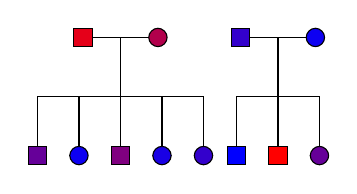
\begin{tikzpicture}[
				man/.style={rectangle,draw},
				woman/.style={rectangle,draw,rounded corners=.8ex},
				first/.style={level distance=6pt},
				level 1/.style={sibling distance=15pt}]
				%level 2/.style={sibling distance=15pt}]
					% Parents
					\uncover<3->{
					\coordinate (family1) at (0,0)
						child[grow=left,level distance=10pt]{node[man,anchor=east,fill=red!90!blue]{}}
						child[grow=right,level distance=10pt]{node[woman,anchor=west,fill=red!70!blue]{}}
						child[grow=down,level distance=0ex]
					[edge from parent fork down]
					% Children and grandchildren
					child{node[man,fill=red!40!blue] {}}
					child{node[woman,fill=red!5!blue] {}}
					child {node[man,fill=red!50!blue] {}}
					child {node[woman,fill=red!10!blue] {}}
					child {node[woman,fill=red!20!blue] {}};
				
				\coordinate (family2) at (2,0)
						child[grow=left,level distance=10pt]{node[man,anchor=east,fill=red!20!blue]{}}
						child[grow=right,level distance=10pt]{node[woman,anchor=west,fill=red!5!blue]{}}
						child[grow=down,level distance=0ex]
					[edge from parent fork down]
					% Children and grandchildren
					child{node[man,fill=red!0!blue] {}}
					child{node[man,fill=red!100!blue] {}}
					child {node[woman,fill=red!40!blue] {}};	}
				\end{tikzpicture}
			\end{figure}
		\end{column}
		\begin{column}[c]{0.5\textwidth}
			\vspace{-10pt}
			\begin{center}
				\uncover<4->{heritability$\approx$1}
			\end{center}
			\vspace{-10pt}
			\begin{figure}
			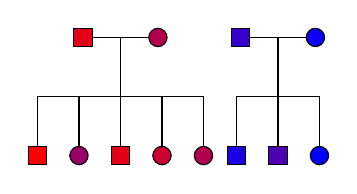
\begin{tikzpicture}[
			man/.style={rectangle,draw},
			woman/.style={rectangle,draw,rounded corners=.8ex},
			first/.style={level distance=6pt},
			level 1/.style={sibling distance=15pt}]
				% Parents
				\uncover<4->{
				\coordinate
					child[grow=left,level distance=10pt]{node[man,anchor=east,fill=red!90!blue]{}}
					child[grow=right,level distance=10pt]{node[woman,anchor=west,fill=red!70!blue]{}}
					child[grow=down,level distance=0ex]
				[edge from parent fork down]
				% Children and grandchildren
				child{node[man,fill=red!99!blue] {}}
				child{node[woman,fill=red!60!blue] {}}
				child {node[man,fill=red!90!blue] {}}
				child {node[woman,fill=red!80!blue] {}}
				child {node[woman,fill=red!70!blue] {}};
			
					\coordinate (family2) at (2,0)
					child[grow=left,level distance=10pt]{node[man,anchor=east,fill=red!20!blue]{}}
					child[grow=right,level distance=10pt]{node[woman,anchor=west,fill=red!5!blue]{}}
					child[grow=down,level distance=0ex]
				[edge from parent fork down]
				% Children and grandchildren
				child{node[man,fill=red!10!blue] {}}
				child{node[man,fill=red!30!blue] {}}
				child {node[woman,fill=red!0!blue] {}};
				}
			\end{tikzpicture}
		\end{figure}
	\end{column}
\end{columns}

\uncover<5->{

\begin{center}
\textbf{Breeding value}\\
= Individual additive genetic value\\
Change with time = evolution
\end{center}
}

\end{frame}
%%%%%%%%%%%

\begin{frame}%break
\end{frame}
%%%%%%%%%%%

\begin{frame}{Adaptive evolution in the wild}
% many examples

\end{frame}
%%%%%%%%%%%

\begin{frame}{Adaptive evolution in the wild}
%but difficult to see it happen live and understand its causes

\begin{center}
	Adaptive evolution = Selection $\times$ heritability
\end{center}

	\only<2>{\begin{figure}
		\fcolorbox{OwlGreen}{OwlGreen}{\includegraphics[width=0.8\textwidth]{Figures/PrimHolstein}}
	\end{figure}}
	
	\only<3>{\begin{figure}
		\fcolorbox{OwlGreen}{OwlGreen}{\includegraphics[width=0.8\textwidth]{Figures/Experimental}}
		
		Experimental evolution. Kawecki \& al. (2012) Trends in Ecology \& Evolution 27(10)
	\end{figure}}
    
\only<4>{
	\begin{figure}
		\fcolorbox{bostonuniversityred}{bostonuniversityred}{\includegraphics[width=0.8\textwidth]{Figures/Wild}}
	\end{figure}}
	
	
\only<5>{
\begin{center}
	2001
\end{center}
	\begin{figure}
			\includegraphics[width=0.8\textwidth]{Figures/Merila2001}
	\end{figure}	}

\only<6>{	
\begin{center}
	2014
\end{center}
	\begin{figure}
			\includegraphics[width=0.8\textwidth]{Figures/Merila2014}
	\end{figure}	}

\only<7>{
\begin{center}
	2016
\end{center}
	\begin{figure}
			\includegraphics[width=0.8\textwidth]{Figures/Brookfield}
	\end{figure}
	\textbf{\color{OwlGreen}{Long-term individual-based monitoring}}
	}

\end{frame} % To do that we need very accurate individual-based monitoring over multiple generations
%%%%%%%%%%%

%%%%%%%%%%%%%%%%%%%%%%%%%%%%%%%%%%%%%%%%%%%%%%%%%%%%%%%%%%%%%%%%%%%%%%%
%%%%%%%%%%%%%%%%%%%%%%%%%%%% Monitoring %%%%%%%%%%%%%%%%%%%%%%%%%%%%%%%
%%%%%%%%%%%%%%%%%%%%%%%%%%%%%%%%%%%%%%%%%%%%%%%%%%%%%%%%%%%%%%%%%%%%%%%

%FIeld and population
\begin{frame}[plain]{}
	\begin{figure}
	\centering
		\includegraphics[height= \textheight]{Figures/SnowBall}
	\end{figure}
\end{frame}
%%%%%%%%%%%

\begin{frame}{Snow vole (\textit{Chionomys nivalis}, Martins 1842)}

\begin{columns}
	\begin{column}[c]{0.5\textwidth}
		\begin{itemize}[<+->]
			\item NOT white
			\item Rock-dweller
			\item 30-45g
			\item 10-14cm long $+$ 5-8cm tail
			\item Slow life pace
		\end{itemize}
	\end{column}
	\begin{column}[c]{0.5\textwidth}
	\begin{figure}
	\centering
		\includegraphics[width= \textwidth]{Figures/P1250035}
	\end{figure}
	\end{column}
	\end{columns}
\end{frame}
%%%%%%%%%%%

\begin{frame}
	\begin{figure}
	\centering
		\includegraphics[height= \textheight]{Figures/map-1}
	\end{figure}
\end{frame}
%%%%%%%%%%%

\begin{frame}
	\begin{figure}
	\centering
		\begin{tikzpicture}
			
			\node (pic) at (0,0) {\includegraphics[width= 0.95\textwidth]{Figures/DSC_2111viewontaliflue}};
			\draw[rounded corners,thick,color=red] (-1.2,-0.8) rectangle (0.5,0);
		\end{tikzpicture}
	\end{figure}
\end{frame}
%%%%%%%%%%%

\begin{frame}
	\begin{figure}
	\centering
		\includegraphics[width= \textwidth]{Figures/fieldposts2}
	\end{figure}
\end{frame}
%%%%%%%%%%%

\begin{frame}
	\begin{figure}
	\centering
		\includegraphics[width= \textwidth]{Figures/boulder}
	\end{figure}
\end{frame}
%%%%%%%%%%%

\begin{frame}
	\begin{figure}
	\centering
		\includegraphics[width= \textwidth]{Figures/DSC_2027trap}
	\end{figure}
\end{frame}
%%%%%%%%%%%

\begin{frame}{What we measure}

\begin{columns}
	\begin{column}[c]{0.4\textwidth}
		\begin{itemize}
			\item<2-> Morphology
				\begin{itemize}
					\item Body mass 
					\item Body length
					\item Tail length
				\end{itemize}
			\item<3-> Capture/Recaptures
				\begin{itemize}
					\item Death/emigration
					\item Location
				\end{itemize}
			\item<4-> DNA
				\begin{itemize}
					\item 20 ``neutral'' markers
					\item Sex identification
					\item Any genotyping
					\item<5-> \textbf{Pedigree}
				\end{itemize}
		\end{itemize}
	\end{column}
	
	\begin{column}[c]{0.6\textwidth}

	\centering
		\only<2>{\includegraphics[height= \textheight]{Figures/CN2015_MeulenbroekLiz_00024}}
		\only<3>{\includegraphics[height= \textheight]{Figures/CN2015_MeulenbroekLiz_00022}}
		\only<4>{\includegraphics[height= \textheight]{Figures/IMG_20160916_075241}}
		\only<5>{\includegraphics[height= 0.5\textheight]{Figures/familytree}}
		\only<6>{\includegraphics[height= \textheight]{Figures/pedigreeplot}}

	\end{column}
\end{columns}
\end{frame}
%%%%%%%%%%%


%%%%%%%%%%%%%%%%%%%%%%%%%%%%%%%%%%%%%%%%%%%%%%%%%%%%%%
%%%%%%%%%%%%%%%%%%%%%%% Chap 3 %%%%%%%%%%%%%%%%%%%%%%%
%%%%%%%%%%%%%%%%%%%%%%%%%%%%%%%%%%%%%%%%%%%%%%%%%%%%%%
\section{Are snow vole evolving? Why?}

\begin{frame}{Variance in fitness?}

\only<2>{\begin{figure}
		\includegraphics[width=0.5\textwidth]{Figures/figure/dice2-4}
	\end{figure}\vspace{-0.5cm}
	\begin{center}
	\begin{table}
\begin{tabular}{c c c c}
\hline 
& Estimate & 95\% CI & p-value\\
\hline
Latent variance in survival & 0 & [0;0.248] & 0.50\\
Latent variance in reproduction & 0.37 & [0.25, 0.49] & $<10^{-16}$\\
\hline
\end{tabular}
\end{table}
\end{center}}

\only<3>{
\begin{columns}
\begin{column}[c]{0.3\textwidth}
\begin{figure}
		\includegraphics[width=0.9\textwidth]{Figures/pedigreeplot}
	\end{figure}
\end{column}
\begin{column}[c]{0.7\textwidth}
	\begin{center}
	Relative lifetime reproductive success\\
	variance $\approx$ 1.7
	\end{center}
	\end{column}
\end{columns}
	}

\only<4>{
\begin{figure}
			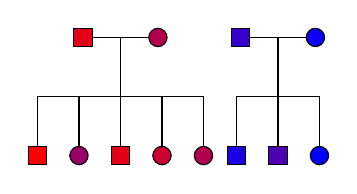
\begin{tikzpicture}[
			man/.style={rectangle,draw},
			woman/.style={rectangle,draw,rounded corners=.8ex},
			first/.style={level distance=6pt},
			level 1/.style={sibling distance=15pt}]
				% Parents
				\coordinate
					child[grow=left,level distance=10pt]{node[man,anchor=east,fill=red!90!blue]{}}
					child[grow=right,level distance=10pt]{node[woman,anchor=west,fill=red!70!blue]{}}
					child[grow=down,level distance=0ex]
				[edge from parent fork down]
				% Children and grandchildren
				child{node[man,fill=red!99!blue] {}}
				child{node[woman,fill=red!60!blue] {}}
				child {node[man,fill=red!90!blue] {}}
				child {node[woman,fill=red!80!blue] {}}
				child {node[woman,fill=red!70!blue] {}};
			
					\coordinate (family2) at (2,0)
					child[grow=left,level distance=10pt]{node[man,anchor=east,fill=red!20!blue]{}}
					child[grow=right,level distance=10pt]{node[woman,anchor=west,fill=red!5!blue]{}}
					child[grow=down,level distance=0ex]
				[edge from parent fork down]
				% Children and grandchildren
				child{node[man,fill=red!10!blue] {}}
				child{node[man,fill=red!30!blue] {}}
				child {node[woman,fill=red!0!blue] {}};
			\end{tikzpicture}
\end{figure}
	\begin{center}
	\begin{table}
		\begin{tabular}{c c c}
		\hline 
		& Estimate & 95\% CI \\
		\hline
		Additive genetic variation & 0.10 & [0.06;0.19] \\
		Heritability & 0.06 & [0.04;0.12] \\
		\hline
		\end{tabular}
	\end{table}
	\end{center}}

\vfill
\begin{block}{Adaptive evolution in the snow vole?}
	\begin{itemize}
		\uncover<2->{\item Non random variation fitness components}
		\uncover<3->{\item Variation in fitness}
		\uncover<4->{\item Additive genetic variation in fitness}
	\end{itemize}
	\centering
	\uncover<5->{\textbf{\alert{On going evolution and opportunity for selection}}}
\end{block}

\end{frame}
%%%%%%%%%%%

%%% Here introduce selection on mass
\begin{frame}{Body mass}
	
\end{frame}

%%%%%%%%%%%
{ % brace to limit the scope of \setbeamertemplate 
\setbeamertemplate{navigation symbols}{}  % optionally hide navigation buttons 
\setbeamertemplate{background canvas}{\includegraphics[width=\paperwidth,height=\paperheight]{Figures/Taliflue-winter.jpg}}
\begin{frame}{Body mass}

\end{frame}
}
%%%%%%%%%%%

\begin{frame}{Evolution of body mass}
	\begin{alertblock}{Prediction}
				\begin{itemize}[<+->]
					\item Selection = +0.86g (p$< 10^{-3}$)
					\item Heritability = 20\% (p$ < 10^{-3}$)
					\item Response = Selection $\times$ heritability = + 0.22g/year
				\end{itemize}
			\end{alertblock}
			
			\uncover<4->{\begin{alertblock}{Phenotypic observation}	
	\begin{columns}
		\begin{column}[c]{0.6\textwidth}
			\begin{figure}
				\includegraphics[width=1\textwidth]{Figures/PhenoTrends-1}
			\end{figure}
		\end{column}
		\begin{column}[c]{0.4\textwidth}
			\begin{itemize}
				\item Observed = +0.07g/year (p=0.14)
			\end{itemize}
		\end{column}
		\end{columns}
	\end{alertblock}}
\end{frame}
%%%%%%%%%%%

\begin{frame}{Evolution of body mass}
\alert{\textbf{Estimation of genetic change}}

\vspace{-0.2cm}

	\begin{figure}
		\includegraphics[width=0.75\textwidth]{Figures/DriftComp-1}
	\end{figure}
\end{frame}
%%%%%%%%%%%
%
\begin{frame}{Evolution of body mass}
\begin{alertblock}{Evolution Paradox}
	\begin{itemize}
		\item Apparent selection for higher mass
		\item Adaptive evolution for lower mass
	\end{itemize}
\end{alertblock}

\uncover<2->{
	\begin{figure}
		\colorbox{white}{\includegraphics[width=0.75\textwidth]{Figures/SelectionTotal-1}}
	\end{figure}}
	
\end{frame}
%%%%%%%%%%%

\begin{frame}
\begin{figure}
\begin{tikzpicture}[]

%\tikzset{>=stealth}

\def\separr{10pt}
\def\separrVoles{12pt}
\def\linew{2pt}
\def\toSelEv{2cm}
\def\lengthgrowth{1.25cm}
\def\betweenGrowth{2cm}

%fitness square
\coordinate (fitbl) at (0,0);
\coordinate (fitbr) at (3,0);
\coordinate (fittl) at (0,3);
\coordinate (fittr) at (3,3);

\uncover<3>{
\shade[shading=axis,right color=mypurple!80!white, left color=mypurple!20!white,shading angle=135] (fitbl) -- (fitbr) -- (fittr) -- (fittl);				
}

\uncover<4->{
\shade[shading=axis,right color=red, left color=red!5!white,shading angle=71.5] (fitbl) -- (fitbr) -- (fittr) -- (fittl);				
}

%fitness square attributes
\uncover<1->{
\draw[->,line width=\linew,color=mygreen] ($(fitbl)-(0,\separr)$)--($(fitbr)-(0,\separr)$);
\node[] (plus) at ($(fitbr)+(0,-2*\separr)$) {$\boldsymbol{+}$};
\node[] (plus) at ($(fitbl)+(0,-2*\separr)$) {$\boldsymbol{-}$};
\node[] (plus) at ($(fitbl)+(1.5,-2.5*\separr)$) {\includegraphics[width=1cm]{Figures/GrassGreen}};}%ENV

\uncover<2->{
\draw[->,line width=\linew,color=myorange] ($(fitbl)-(\separr,0)$)--($(fittl)-(\separr,0)$);
\node[] (plus) at ($(fittl)+(-2*\separr,0)$) {$\boldsymbol{+}$};
\node[] (plus) at ($(fitbl)+(-2*\separr,0)$) {$\boldsymbol{-}$};
\node[] (plus) at ($(fitbl)+(-2.5*\separr,1.5)$) {\includegraphics[width=1cm]{Figures/dnaOrange}};}%DNA

\uncover<6->{
\foreach \x in {1,2,3} {
	\draw[color=white,line width=1pt] ($(fitbl)+(\x-1,0)$) -- ($(fittl)+(\x,0)$);
	}
	}

\uncover<5->{
\foreach \x in {1,2,3} {
	\draw[color=mypurple,line width=1pt] ($(fitbl)+(\x,0)$) -- ($(fitbl)+(0,\x)$);
	}
\foreach \x in {1,2} {
	\draw[color=mypurple,line width=1pt] ($(fittr)-(\x,0)$) -- ($(fittr)-(0,\x)$);
	}
	\node[rotate=315,color=mypurple] (fitiso) at (0.9,1.3) {mass isolines};
	}
	
	\uncover<6->{\node[rotate=71.5,color=white] (fitiso) at (2.2,1.15) {fitness isolines};
	}



\uncover<1->{
\node[] (svsmall) at ($(fitbl)+(\separrVoles,\separrVoles)$) {\includegraphics[width=0.7cm]{Figures/Snowvoleshadow}};}

\uncover<4->{\node[] (juv) at ($(svsmall)+(-0.05,-0.25)$) {\includegraphics[width=0.25cm]{Figures/JuvVole}};
\node[] (juv) at ($(svsmall)+(0.25,-0.3)$) {\includegraphics[width=0.25cm]{Figures/JuvVole}};}

\uncover<2->{
\node[] (svmed1) at ($(fittl)+(\separrVoles,-\separrVoles)$) {\includegraphics[width=1.3cm]{Figures/Snowvoleshadow}};}
\uncover<4->{\node[] (juv) at ($(svmed1)+(-0.1,-0.3)$) {\includegraphics[width=0.25cm]{Figures/JuvVole}};}

\uncover<1->{
\node[] (svsmed2) at ($(fitbr)+(-\separrVoles,\separrVoles)$) {\includegraphics[width=1.3cm]{Figures/Snowvoleshadow}};}
\uncover<4->{\node[] (juv) at ($(svsmed2)+(0,-0.3)$) {\includegraphics[width=0.25cm]{Figures/JuvVole}};
\node[] (juv) at ($(svsmed2)+(-0.3,-0.3)$) {\includegraphics[width=0.25cm]{Figures/JuvVole}};
\node[] (juv) at ($(svsmed2)+(0.3,-0.3)$) {\includegraphics[width=0.25cm]{Figures/JuvVole}};
\node[] (juv) at ($(svsmed2)+(-0.27,0)$) {\includegraphics[width=0.25cm]{Figures/JuvVole}};}

\uncover<3->{
\node[] (svbig) at ($(fittr)+(-\separrVoles,-\separrVoles)$) {\includegraphics[width=2cm]{Figures/Snowvoleshadow}};}
\uncover<4->{\node[] (juv) at ($(svbig)+(-0.35,0.2)$) {\includegraphics[width=0.25cm]{Figures/JuvVole}};
\node[] (juv) at ($(svbig)+(-0.3,-0.3)$) {\includegraphics[width=0.25cm]{Figures/JuvVole}};
\node[] (juv) at ($(svbig)+(-0.35,-0.05)$) {\includegraphics[width=0.25cm]{Figures/JuvVole}};}

%Selection
\coordinate (SelOr) at ($(fittr)+(\toSelEv,-0.5)$);
\coordinate (SelY) at ($(SelOr)+(0,1)$);
\coordinate (SelX) at ($(SelOr)+(1,0)$);

\uncover<7->{
\draw[->,color=mypurple,thick] (SelOr)--(SelX);
\draw[->,thick] (SelOr)--(SelY);
%\node[anchor=north] (SellabX) at (SelX) {Mass};
\node[anchor=north] (SelVolL) at ($(SelOr)+(0,0.1)$) {\includegraphics[width=0.7cm]{Figures/Snowvoleshadow}};
\node[anchor=north] (SelVolH) at ($(SelX)+(0,0.3)$) {\includegraphics[width=2cm]{Figures/Snowvoleshadow}};

\node[anchor=east,rotate=90] (SellabY) at ($(SelY)+(-0.22,0.1)$) {Fitness};


\draw[color=red] ($(SelOr)+(0.1,0.2)$)--($(SelOr)+(0.9,0.8)$);
}
%\node[anchor=south] (sfhv) at ($(SelY)+(0,0.5)$) {Selection for heavier voles};

%Sel on genes
\coordinate (SGOr) at ($(fitbr)+(\toSelEv,-0.5)$);
\coordinate (SGY) at ($(SGOr)+(0,1)$);
\coordinate (SGX) at ($(SGOr)+(1,0)$);

\uncover<8->{
\draw[->,thick,color=myorange] (SGOr)--(SGX);
\draw[->,thick] (SGOr)--(SGY);
\node[anchor=west] (SGlabX) at ($(SGX)+(-0.2,0)$) {\includegraphics[width=0.5cm]{Figures/dnaOrange}};
\node[anchor=east,rotate=90] (SGlabY) at ($(SGY)+(-0.22,0.1)$){Fitness};

\draw[color=red] ($(SGOr)+(0.1,0.8)$)--($(SGOr)+(0.9,0.2)$);
}

%Evolution
\coordinate (EvOr) at ($(SGOr)+(2.5,0)$);
\coordinate (EvY) at ($(EvOr)+(0,1)$);
\coordinate (EvX) at ($(EvOr)+(1,0)$);

\uncover<9->{
\draw[->,thick] (EvOr)--(EvX);
\draw[->,thick,color=myorange] (EvOr)--(EvY);
\node[anchor=north] (EvlabX) at (EvX) {Year};
\node[anchor=east] (EvlabY) at ($(EvY)+(0.2,0)$) {\includegraphics[width=0.5cm]{Figures/dnaOrange}};

\draw[color=red] ($(EvOr)+(0.1,0.8)$)--($(EvOr)+(0.9,0.2)$);
}				
%\node[anchor=north] (eflv) at ($(EvOr)+(0,-0.5)$) {Evolution for lighter voles};

				
%To Sel and Ev
\coordinate (cross) at ($(fittr)+(\toSelEv/3,-1.5)$);

\uncover<7->{
\draw[->,line width=4pt]	($(cross)+(-0.5,0)$)--(cross)--($(SelOr)+(-0.5,0)$);}

\uncover<8->{
\draw[->,line width=4pt]	(cross)--($(SGOr)+(-0.5,1)$);}

\uncover<9->{
\draw[->,line width=4pt] ($(SGX)+(0.5,0.5)$) -- ($(EvOr)+(-0.5,0.5)$);}
%to matrix
%\draw[->,line width=4pt]	($(G1X)+(0.2,0)$)--($(cross)+(-5.4,0)$);

%%%%%%%%%%%%%%%%%%%%%
%\node[anchor=south] (snow) at ($(fittl)+(1.25,0.5)$) {\includegraphics[width=5cm]{BDsnow-1}};
%\node[] (birth) at ($(snow)+(-6,0)$) {\includegraphics[width=5cm]{Climatic_trend-1}};
%
%\draw[->,line width=4pt]	($(snow.west)$)--($(birth.east)$);
%\draw[->,line width=4pt]	($(birth.south)$)--($(birth.south)+(0,-0.5)$);
				

				
\end{tikzpicture}

\end{figure}
\uncover<10->{
\begin{alertblock}{Summary}
	\begin{enumerate}
		\uncover<10->{\item Apparent stasis\dots}
		\uncover<11->{\item \dots but evolution towards lower mass}
		\uncover<12->{\item \textit{Selective pressure?}}
	\end{enumerate}
\end{alertblock}
} 
\end{frame}
%%%%%%%%%%%

\begin{frame}{}
	\begin{figure}
		\colorbox{white}{\includegraphics[width=\textwidth]{Figures/SelectionS-1}}
	\end{figure}
\end{frame}
%%%%%%%%%%%

\begin{frame}{}
\frametitle{Snow falls and ontogeny}

	\begin{figure}
		\colorbox{white}{\includegraphics[width=0.5\textwidth]{Figures/BDsnow-1}
		\uncover<2->{\includegraphics[width=0.5\textwidth]{Figures/Climatic_trend-1}}}
	\end{figure}
	\uncover<3->{\alert{Less time to grow $\rightarrow$ Selection for smaller voles?}}
\end{frame}
%%%%%%%%%%%

\begin{frame}{Selection during ontogeny?}
\begin{figure}
\begin{tikzpicture}[]

\def\separr{10pt}
\def\separrVoles{12pt}
\def\linew{2pt}
\def\toSelEv{2cm}
\def\lengthgrowth{1.25cm}
\def\betweenGrowth{2.3cm}

%fitness square
\coordinate (fitbl) at (0,0);

%Growth curves%%%%%%%%%%%%%%%%%%%%%%%

%First growth curves
\coordinate (G1OR) at ($(fitbl)+(-4,1.5)$);
\coordinate (G1Y) at ($(G1OR)+(0,1)$);
\coordinate (G1X) at ($(G1OR)+(\lengthgrowth,0)$);
\node[] (D) at ($(G1OR)+(-0.25*\lengthgrowth,1.65)$) {\large \textbf{D}};

\uncover<3->{
%\draw[black,domain=-3:-2] plot (\x,{1.5*(2-exp(-0.2*(\x)))});
\draw[color=mypurple1,thick] (G1OR) to[out=0,in=235] ($(G1OR)+(0.4,0.2)$);
\draw[color=mypurple1,thick] ($(G1OR)+(0.4,0.2)$) to[out=55,in=180] ($(G1X)+(-0.6,0.4)$) ;
\draw[color=mypurple1,thick] ($(G1X)+(-0.61,0.4)$)--($(G1X)+(0,0.4)$) ;

\draw[color=mypurple1,thick] ($(G1OR)+(0.4,0)$) to[out=0,in=235] ($(G1OR)+(0.8,0.2)$);
\draw[color=mypurple1,thick] ($(G1OR)+(0.8,0.2)$) to[out=55,in=180] ($(G1X)+(-0.2,0.4)$);

\draw[color=mypurple2,thick] (G1OR) to[out=0,in=245] ($(G1OR)+(0.5,0.45)$);
\draw[color=mypurple2,thick] ($(G1OR)+(0.5,0.45)$) to[out=65,in=190] ($(G1X)+(-0.4,0.9)$) ;
\draw[color=mypurple2,thick] ($(G1X)+(-0.41,0.9)$)--($(G1X)+(0,0.9)$) ;

\draw[color=mypurple2,thick] ($(G1OR)+(0.4,0)$) to[out=0,in=245] ($(G1OR)+(0.9,0.45)$);
\draw[color=mypurple2,thick] ($(G1OR)+(0.9,0.45)$) to[out=65,in=240] ($(G1OR)+(0.99,0.65)$);
\draw[color=mypurple2,thick,densely dotted] ($(G1OR)+(0.9,0.45)$) to[out=65,in=190] ($(G1X)+(0,0.9)$) ;

\draw[->] (G1OR)--(G1Y);
\draw[->] (G1OR)--(G1X);
\node[anchor=north] (ttime1) at ($(G1X)+(-0.5,0)$) {time};
\draw[color=blue] ($(G1OR)+(0.97,0)$)--($(G1OR)+(0.97,1.1)$);
%\draw[color=blue,->] ($(G1OR)+(1.0,1.12)$)--($(G1OR)+(1.5,1.12)$);
%\node[color=blue] (wint1) at ($(G1OR)+(1.2,1.2)$) {\tiny winter};
%\node[anchor=south] (mm1) at (G1Y) {Mass};

\node[] (svl1) at ($(G1X)+(0.2,0.4)$) {\includegraphics[width=0.6cm]{Figures/SnowvoleshadowLight}};
\node[] (svh1) at ($(G1X)+(0.2,0.9)$) {\includegraphics[width=1cm]{Figures/SnowvoleshadowDark}};
}
%Second growth curves
\coordinate (G2OR) at ($(G1OR)+(-\betweenGrowth,0)$);
\coordinate (G2Y) at ($(G2OR)+(0,1)$);
\coordinate (G2X) at ($(G2OR)+(\lengthgrowth,0)$);

\uncover<1->{
\draw[color=mypurple1,thick] (G2OR) to[out=0,in=235] ($(G2OR)+(0.4,0.2)$);
\draw[color=mypurple1,thick] ($(G2OR)+(0.4,0.2)$) to[out=55,in=180] ($(G2X)+(-0.6,0.4)$) ;
\draw[color=mypurple1,thick] ($(G2X)+(-0.61,0.4)$)--($(G2X)+(0,0.4)$) ;

\draw[color=mypurple1,thick] ($(G2OR)+(0.4,0)$) to[out=0,in=235] ($(G2OR)+(0.8,0.2)$);
\draw[color=mypurple1,thick] ($(G2OR)+(0.8,0.2)$) to[out=55,in=180] ($(G2X)+(-0.2,0.4)$);

\draw[color=mypurple2,thick] (G2OR) to[out=0,in=245] ($(G2OR)+(0.5,0.45)$);
\draw[color=mypurple2,thick] ($(G2OR)+(0.5,0.45)$) to[out=65,in=190] ($(G2X)+(-0.4,0.9)$) ;
\draw[color=mypurple2,thick] ($(G2X)+(-0.41,0.9)$)--($(G2X)+(0,0.9)$) ;

\draw[color=mypurple2,thick] ($(G2OR)+(0.4,0)$) to[out=0,in=245] ($(G2OR)+(0.9,0.45)$);
\draw[color=mypurple2,thick] ($(G2OR)+(0.9,0.45)$) to[out=65,in=190] ($(G2X)+(0,0.9)$) ;

\draw[->] (G2OR)--(G2Y);
\draw[->] (G2OR)--(G2X);


\node[anchor=north] (ttime2) at ($(G2X)+(-0.5,0)$) {time};
\node[anchor=315,rotate=90] (mm2) at ($(G2Y)+(0,-0.25)$) {mass};

\node[] (svl2) at ($(G2X)+(0.2,0.4)$) {\includegraphics[width=0.6cm]{Figures/SnowvoleshadowLight}};
\node[] (svh2) at ($(G2X)+(0.2,0.9)$) {\includegraphics[width=1cm]{Figures/SnowvoleshadowDark}};

\draw[color=blue] ($(G2OR)+(1.15,0)$)--($(G2OR)+(1.15,1.1)$);
}
%%%Histograms %%%%%%%%%%%%%%%%%
%First hist
\coordinate (H1OR) at ($(G1OR)+(0,-2)$);
\coordinate (H1Y) at ($(H1OR)+(0,1)$);
\coordinate (H1X) at ($(H1OR)+(\lengthgrowth,0)$);

%\node[anchor=south] (mm2) at (H1Y) {Freq.};
\uncover<4->{
\draw[color=mypurple1,fill=mypurple1] ($(H1OR)+(0.3,0)$) -- ($(H1OR)+(0.5,0)$) -- ($(H1OR)+(0.5,0.67)$) -- ($(H1OR)+(0.3,0.67)$) -- ($(H1OR)+(0.3,0)$);

\draw[color=mypurple2,fill=mypurple2] ($(H1OR)+(0.8,0)$) -- ($(H1OR)+(1,0)$) -- ($(H1OR)+(1,0.33)$) -- ($(H1OR)+(0.8,0.33)$) -- ($(H1OR)+(0.8,0)$);
\draw[->] (H1OR)--(H1Y);
\draw[] (H1OR)--(H1X);
\node[anchor=45] (gl1) at ($(H1OR)+(0.6,0.1)$) {\includegraphics[width=0.6cm]{Figures/SnowvoleshadowLight}};
\node[anchor=45] (gh1) at ($(H1OR)+(1.3,0.2)$) {\includegraphics[width=1cm]{Figures/SnowvoleshadowDark}};

\draw[color=red,thick] ($(H1OR)+(0,0.7)$) -- ($(H1X)+(0,0.35)$);
\node[color=red,anchor=south,rotate=345] (yos) at ($(H1OR)+(\lengthgrowth/2,0.55)$) {\tiny selection};
}
%Second hist
\coordinate (H2OR) at ($(G2OR)+(0,-2)$);
\coordinate (H2Y) at ($(H2OR)+(0,1)$);
\coordinate (H2X) at ($(H2OR)+(\lengthgrowth,0)$);

\uncover<2->{
\node[anchor=315,rotate=90] (mm2) at ($(H2Y)+(0,-0.25)$) {fitness};
\draw[color=darkred,thick] ($(H2OR)+(0,0.55)$) -- ($(H2X)+(0,0.55)$);
\node[color=darkred,anchor=south] (nos) at ($(H2OR)+(\lengthgrowth/2,0.55)$) {\tiny no selection};

\draw[color=mypurple1,fill=mypurple1] ($(H2OR)+(0.3,0)$) -- ($(H2OR)+(0.5,0)$) -- ($(H2OR)+(0.5,0.5)$) -- ($(H2OR)+(0.3,0.5)$) -- ($(H2OR)+(0.3,0)$);

\draw[color=mypurple2,fill=mypurple2] ($(H2OR)+(0.8,0)$) -- ($(H2OR)+(1,0)$) -- ($(H2OR)+(1,0.5)$) -- ($(H2OR)+(0.8,0.5)$) -- ($(H2OR)+(0.8,0)$);

\draw[->] (H2OR)--(H2Y);
\draw[] (H2OR)--(H2X);

\node[anchor=45] (gl2) at ($(H2OR)+(0.6,0.1)$) {\includegraphics[width=0.6cm]{Figures/SnowvoleshadowLight}};
\node[anchor=45] (gh2) at ($(H2OR)+(1.3,0.2)$) {\includegraphics[width=1cm]{Figures/SnowvoleshadowDark}};
}
%Boxes
\draw[rounded corners] ($(G1X)+(0.8,1.3)$) rectangle ($(H1OR)+(-0.2,-1.5)$);
\draw[rounded corners] ($(G1X)+(-1.7,1.3)$) rectangle ($(H2OR)+(-0.5,-1.5)$);
\node[anchor=south] (p1) at ($(H1OR)+(0.9,-1.5)$) {2008-2014};
\node[anchor=south] (p1) at ($(H2OR)+(0.7,-1.5)$) {2006-2007};

\uncover<5>{
\node[anchor=west] (phiam) at ($(H1OR)+(2.5,1)$) {\colorbox{white}{\includegraphics[width=6cm]{Figures/PhiAM-4}}};
}
\uncover<6>{
\node[anchor=west] (phiam) at ($(H1OR)+(2.5,1)$) {\colorbox{white}{\includegraphics[width=6cm]{Figures/PhiAM-9}}};
}
\uncover<7>{
\node[anchor=west] (phiam) at ($(H1OR)+(2.5,1)$) {\colorbox{white}{\includegraphics[width=6cm]{Figures/PhiAM-13}}};
}
\end{tikzpicture}

\end{figure}
\end{frame}
%%%%%%%%%%%

\begin{frame}{E{\color{OwlRed}{vole}}ution!}

		\begin{itemize}
			\uncover<2->{\item Contemporary adaptive evolution}
			\uncover<3->{\item Against apparent selection}
			\uncover<4->{\item In response to climate}
		\end{itemize}

	\uncover<5->{\begin{figure}
		\includegraphics[width=\textwidth]{Figures/SelRepSel}
	\end{figure} \vspace{-0.8cm}}
\end{frame}
%%%%%%%%%%%

%%%%%%%%%%%%%%%%%%%%%%%%%%%%%%%%%%%%%%%%%%%%%%%%%%%%%%
%%%%%%%%%%%%%%%%%%%%%%% Chap 4 %%%%%%%%%%%%%%%%%%%%%%%
%%%%%%%%%%%%%%%%%%%%%%%%%%%%%%%%%%%%%%%%%%%%%%%%%%%%%%

\section{Do selection and evolution fluctuate?}

\begin{frame}

\begin{columns}
	\begin{column}[c]{0.5\textwidth}
	\begin{figure}
	Selection
		\begin{tikzpicture}
			\coordinate (o) at (0,0);
			\coordinate (x) at (4,0);
			\coordinate (y) at (0,2);
			\coordinate (ym) at (0,-2);
			
			\uncover<2->{\draw[->] (o) -- (x);
			\draw[->] (ym) -- (y);
			
			\draw[dashed, color=OwlGreen] (0, 0.86) -- (4, 0.86);
			
						\foreach \j in {1,...,4}
				{
				\node[rotate=-45] (lab\j) at ($(\j	,0)+(-0.5,-0.5)$) {\pgfmathparse{2005+\j}% Evaluate the expression
				    \pgfmathprintnumber[    % Print the result
        fixed,
        fixed zerofill,
        precision=0
    ]{\pgfmathresult}};
				}
			}
			\uncover<3->{
			\foreach \Ctest[count=\i] in {1.6,-0.8,0.6, 2}
				{
					\draw (\i-0.5,0) -- (\i-0.5, -0.1);
					%\node[rotate=-45] (year\i) at ($(\i	,0)+(-0.5,-0.5)$) {\pgfmathparse{2005+\i}% Evaluate the expression
    %\pgfmathprintnumber[    % Print the result
    %    fixed,
    %    fixed zerofill,
    %    precision=0
    %]{\pgfmathresult}};
		
			\draw[thick, color = OwlGreen] (\i-0.5,0) -- (\i-0.5, \Ctest);
				}
				}
		\end{tikzpicture}
	\end{figure}
	\end{column}
	\begin{column}[c]{0.5\textwidth}
		\begin{figure}
		\uncover<4->{Evolution}
		\begin{tikzpicture}
			\coordinate (o) at (0,0);
			\coordinate (x) at (4,0);
			\coordinate (y) at (0,2);
			\coordinate (ym) at (0,-2);
			\uncover<5->{
			\draw[->] (o) -- (x);
			\draw[->] (ym) -- (y);
			
			
			\foreach \Ctest[count=\i] in {1.6,-0.8,0.6, 2}
				{
					\draw (\i-0.5,0) -- (\i-0.5, -0.1);
					\node[rotate=-45] (year\i) at ($(\i	,0)+(-0.5,-0.5)$) {\pgfmathparse{2005+\i}% Evaluate the expression
    \pgfmathprintnumber[    % Print the result
        fixed,
        fixed zerofill,
        precision=0
    ]{\pgfmathresult}};
		}
			
		\draw[thick, color=OwlGreen, fill=OwlGreen] (0.5,1) circle [radius=0.1];
		\draw[thick, color=OwlGreen, fill=OwlGreen] (3.5,-1.5) circle [radius=0.1];
		\draw[dashed, color =OwlGreen] (0.5,1) -- (3.5, -1.5);
		}
		\uncover<6->{
		\draw[thick, color = OwlGreen] (0.5,1) -- (1.5,-1);
		\draw[thick, color = OwlGreen] (1.5,-1) -- (2.5,1.8);
		\draw[thick, color = OwlGreen] (2.5,1.8)--(3.5,-1.5);}
		\end{tikzpicture}
	\end{figure}
	\end{column}
\end{columns}
\end{frame}
%%%%%%%%%%%

\begin{frame}{Dynamics of selection}
	\begin{figure}
		\includegraphics[width=0.9\textwidth]{Figures/SelByYear-1}
	\end{figure} \vspace{-0.2cm}
	Variance in selection = 0.117 [0.063;0.218], p=$8\cdot10^{-6}$
\end{frame}
%%%%%%%%%%%

\begin{frame}{Dynamics of evolution}
	\begin{figure}
		\includegraphics[width=\textwidth]{Figures/EvolSmooth-1}
	\end{figure}
\end{frame}
%%%%%%%%%%%

\begin{frame}{Dynamics of selection VS. evolution}
	\begin{figure}
		\includegraphics[width=\textwidth]{Figures/Betas-1}
	\end{figure}
\end{frame} 
%%%%%%%%%%%

\begin{frame}{Dynamics of selection VS. evolution}

	\begin{itemize}[<+->]
		\item Selection fluctuates
		\item Evolution does not
		\item Selection does not predict evolution
	\end{itemize}
	
	\uncover<4->{
	\begin{center}
		\textbf{\large Fluctuating selection but no fluctuating evolution in a wild rodent population}\\
		Timoth\'ee Bonnet \& Erik Postma\\
		Submitted to Evolution
	\end{center}}
\end{frame}

%%%%%%%%%%%%%%%%%%%%%%%%%%%%%%%%%%%%%%%%%%%%%%%%%%%%%%
%%%%%%%%%%%%%%%%%%%%%%% Conclu %%%%%%%%%%%%%%%%%%%%%%%
%%%%%%%%%%%%%%%%%%%%%%%%%%%%%%%%%%%%%%%%%%%%%%%%%%%%%%

\section{Conclusion}
\begin{frame}{Summary}
	
\end{frame}
%%%%%%%%%%%
\begin{frame}{What is left?}
	\begin{exampleblock}{Causes of variation in fitness}
		\begin{itemize}
			\item The genes of others
			\item Molecular basis
		\end{itemize}
	\end{exampleblock}
	%
	\begin{exampleblock}{Predicting responses to environmental change}
		\begin{itemize}
			\item Selection \& evolution in the wild
			\item Demographic response
		\end{itemize}
	\end{exampleblock}
\end{frame}
%%%%%%%%%%%

\section{Questions?}

\end{document}
